\chapter[APLICACIONES DEL ÁLGEBRA LINEAL]{APLICACIONES DEL \\ ÁLGEBRA LINEAL}

Este capítulo presenta ocho aplicaciones del álgebra lineal, cada una desarrollada en una sección independiente. Esto permite al lector abordar las secciones en el orden que prefiera, o incluso ignorar aquellas que no considere relevantes, según sus intereses o necesidades. El objetivo principal es mostrar cómo el álgebra lineal puede aplicarse en distintos contextos, destacando su versatilidad y utilidad.

Dado el enfoque práctico del capítulo, algunas demostraciones han sido omitidas para no desviar la atención del lector. Sin embargo, los resultados necesarios de otros campos se enuncian de manera clara y precisa, acompañados de explicaciones que, cuando es posible, ayudan a comprender su importancia en el contexto presentado. De este modo, el capítulo encuentra un equilibrio entre la formalidad y la claridad, ofreciendo una experiencia valiosa tanto para estudiantes que desean aprender los conceptos básicos del álgebra lineal como para profesionales interesados en sus aplicaciones prácticas.

\section{Construcción de curvas y superficies a través de puntos específicos}

En esta sección describimos una técnica que utiliza determinantes para construir rectas, círculos y secciones cónicas generales que pasan por puntos específicos en el plano. Este procedimiento también se emplea para trazar planos y esferas en el espacio tridimensional que pasan por puntos fijos.

\newpage

\begin{theorem}{}{}
    Un sistema lineal homogéneo con tantas ecuaciones como incógnitas tiene una solución no trivial si y solo si el determinante de la matriz de coeficientes es cero.
\end{theorem}

Mostraremos ahora cómo este resultado puede utilizarse para determinar ecuaciones de varias curvas y superficies que pasan por puntos específicos.

\subsection*{Una línea a través de dos puntos}

Supongamos que $(x_1, y_1)$ y $(x_2, y_2)$ son dos puntos distintos en el plano. Existe una única recta\sideFigure[\label{fig:rectadospuntos}]{
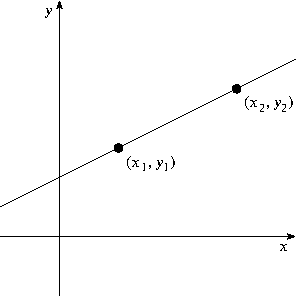
\includegraphics[page=1]{Images/Capitulo8/figurasC8.pdf}
}
\begin{equation}
    c_1x + c_2y + c_3 = 0 \label{recta1}
\end{equation}
que pasa por estos dos puntos (figura \ref{fig:rectadospuntos}). Nótese que $c_1$, $c_2$ y $c_3$ no son todos iguales a cero y que estos coeficientes son únicos hasta una constante multiplicativa. Debido a que $(x_1, y_1)$ y $(x_2, y_2)$ están en la recta, al sustituirlos en \eqref{recta1} obtenemos las dos ecuaciones
\begin{align}
    c_1x_1 + c_2y_1 + c_3 & = 0 \label{recta2} \\
    c_1x_2 + c_2y_2 + c_3 & = 0 \label{recta3}
\end{align}
Las tres ecuaciones, \eqref{recta1}, \eqref{recta2} y \eqref{recta3}, pueden agruparse y reescribirse como
\begin{align*}
    x c_1 + y c_2 + c_3 & = 0 \\
    x_1 c_1 + y_1 c_2 + c_3 & = 0 \\
    x_2 c_1 + y_2 c_2 + c_3 & = 0
\end{align*}
Esto constituye un sistema lineal homogéneo de tres ecuaciones para $c_1$, $c_2$ y $c_3$. Debido a que $c_1$, $c_2$ y $c_3$ no son todos cero, este sistema tiene una solución no trivial, por lo que el determinante de la matriz de coeficientes del sistema debe ser cero. Es decir,
\begin{matriz}
    \makecell{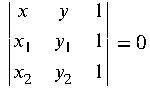
\includegraphics[page=1]{Externalizacion/C8/MatricesC8.pdf}} \label{recta4}
\end{matriz}
En consecuencia, cada punto $(x, y)$ en la recta satisface la ecuación \eqref{recta4}; y, de manera inversa, se puede demostrar que cada punto $(x, y)$ que satisface \eqref{recta4} pertenece a la recta.

\begin{examplebox}{}{}
    Encuentra la ecuación de la recta que pasa por los dos puntos $(2, 1)$ y $(3, 7)$.

    \tcblower
    \solucion Sustituyendo las coordenadas de los dos puntos en la ecuación \eqref{recta4}, obtenemos
    \begin{matrizn}
        \makecell{\includegraphics[page=2]{Externalizacion/C8/MatricesC8.pdf}}
    \end{matrizn}
    La expansión de este determinante a lo largo de la primera fila da como resultado
    $$-6x + y + 11 = 0.$$
\end{examplebox}

\subsection*{Un círculo a través de tres puntos}

Supongamos que hay tres puntos distintos en el plano, $(x_1, y_1)$, $(x_2, y_2)$ y $(x_3, y_3)$, que no están todos en una misma línea recta. De la geometría analítica sabemos que existe un círculo único, de la forma,
\begin{equation}
    c_1\left(x^2 + y^2\right) + c_2x + c_3y + c_4 = 0 \label{circulo5}
\end{equation}
que pasa a través de dichos puntos (figura \ref{fig:circulotrespuntos}). Sustituyendo las coordenadas de los
\newpage
\sideFigure[\label{fig:circulotrespuntos}]{
\includegraphics[page=2]{Images/Capitulo8/figurasC8.pdf}
}
\noindent tres puntos en esta ecuación, obtenemos
\begin{align}
    c_1\left(x_1^2 + y_1^2\right) + c_2x_1 + c_3y_1 + c_4 & = 0 \label{circulo6} \\
    c_1\left(x_2^2 + y_2^2\right) + c_2x_2 + c_3y_2 + c_4 & = 0 \label{circulo7} \\
    c_1\left(x_3^2 + y_3^2\right) + c_2x_3 + c_3y_3 + c_4 & = 0 \label{circulo8}
\end{align}
Como antes, las ecuaciones \eqref{circulo5} a \eqref{circulo8} forman un sistema lineal homogéneo con una solución no trivial para $c_1$, $c_2$, $c_3$ y $c_4$. Por lo tanto, el determinante de la matriz de coeficientes debe ser cero
\begin{matriz}
    \makecell{\includegraphics[page=3]{Externalizacion/C8/MatricesC8.pdf}} \label{circulo9}
\end{matriz}
Esta es la forma de obtener la ecuación del círculo.

\begin{examplebox}{}{}
    Encuentra la ecuación del círculo que pasa por los tres puntos $(1, 7)$, $(6, 2)$ y $(4, 6)$.

    \tcblower
    \solucion Sustituyendo las coordenadas de los tres puntos en la ecuación \eqref{circulo9},
    \begin{matrizn}
        \makecell{\includegraphics[page=4]{Externalizacion/C8/MatricesC8.pdf}}
    \end{matrizn}
    Al simplificar, esto se reduce a
    $$10\left(x^2 + y^2\right) - 20x - 40y - 200 = 0$$
    En su forma estándar, esta ecuación se escribe como
    $$(x - 1)^2 + (y - 2)^2 = 5^2$$
    Por lo tanto, el círculo tiene centro en $(1, 2)$ y radio $5$.
\end{examplebox}

\subsection*{Sección cónica general a través de cinco puntos}

En su monumental obra \emph{Principia Mathematica}, Isaac Newton planteó y resolvió el siguiente problema (Libro I, Proposición 22, Problema 14): “Describir una cónica que pase por cinco puntos dados”. Newton resolvió este problema geométricamente, como se muestra en la figura \ref{fig:conica5puntosN}, en la que hizo pasar una elipse por los puntos A, B, D, P, C; sin embargo, los métodos de esta sección también pueden aplicarse.
\begin{figure}[h!]
    \centering
    \includegraphics[page=3]{Images/Capitulo8/figurasC8.pdf}
    \caption{}\label{fig:conica5puntosN}
\end{figure}

La ecuación general de una sección cónica en el plano (una parábola, hipérbola, elipse o formas degeneradas de estas curvas) está dada por
$$c_1x^2 + c_2xy + c_3y^2 + c_4x + c_5y + c_6 = 0.$$
\newpage\noindent
Esta ecuación contiene seis coeficientes, pero podemos reducir su número a cinco si dividimos entre alguno de ellos que no sea cero. Por lo tanto, solo se necesitan cinco puntos distintos en el plano para determinar la ecuación de la sección cónica. Como antes, la ecuación puede escribirse en forma de determinante:
\begin{matriz}
    \makecell{\includegraphics[page=5]{Externalizacion/C8/MatricesC8.pdf}} \label{conica10}
\end{matriz}

\begin{examplebox}{}{}
    Un astrónomo que desea determinar la órbita de un asteroide alrededor del Sol establece un sistema de coordenadas cartesianas en el plano de la órbita con el Sol en el origen. Se utilizan unidades astronómicas de medida a lo largo de los ejes (1 unidad astronómica = distancia media de la Tierra al Sol = 93 millones de millas). Según la primera ley de Kepler, la órbita debe ser una elipse, por lo que el astrónomo realiza cinco observaciones del asteroide en cinco momentos diferentes y encuentra cinco puntos a lo largo de la órbita
    \begin{gather*}
        (8.025, 8.310), \qquad (10.170, 6.355), \qquad (11.202, 3.212), \\
        (10.736, 0.375), \qquad (9.092, -2.267).
    \end{gather*}
    Determinar la ecuación de la órbita.

    \tcblower
    \solucion Sustituyendo las coordenadas de los cinco puntos dados en la ecuación \eqref{conica10} y redondeando a tres cifras decimales obtenemos
    \begin{matrizn}
        \makecell{\includegraphics[page=6]{Externalizacion/C8/MatricesC8.pdf}}
    \end{matrizn}
    La expansión del determinante por la primera fila produce
    $$386.802x^2 - 102.895xy + 446.029y^2 - 2476.443x - 1427.998y - 17109.375 = 0$$
    La figura \ref{fig:orbita} es un diagrama preciso de la órbita, junto con los cinco puntos.
    \begin{center}
        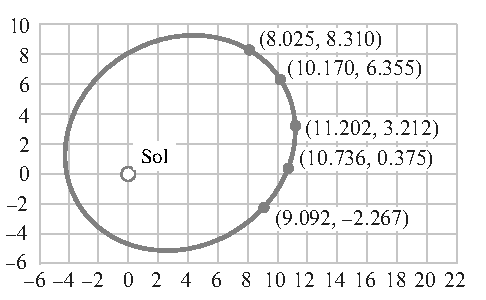
\includegraphics[width=0.75\textwidth]{Images/Capitulo8/Orbita.pdf}
        \captionof{figure}{} \label{fig:orbita}
    \end{center}
\end{examplebox}

\newpage

\subsection*{Un plano a través de tres puntos}

En el ejercicio 8 se deja al lector demostrar lo siguiente: el plano en el espacio tridimensional con ecuación
$$c_1x + c_2y + c_3z + c_4 = 0$$
que pasa por tres puntos no colineales $(x_1, y_1, z_1)$, $(x_2, y_2, z_2)$ y $(x_3, y_3, z_3)$ está dado por la ecuación determinante
\begin{matriz}
    \makecell{\includegraphics[page=7]{Externalizacion/C8/MatricesC8.pdf}} \label{plane11}
\end{matriz}

\begin{examplebox}{}{}
    La ecuación del plano que pasa por los tres puntos no colineales $(1, 1, 0)$, $(2, 0, -1)$ y $(2, 9, 2)$ es
    \begin{matrizn}
        \makecell{\includegraphics[page=8]{Externalizacion/C8/MatricesC8.pdf}}
    \end{matrizn}
    lo que se reduce a
    $$2x - y + 3z - 1 = 0.$$
\end{examplebox}

\subsection*{Una esfera a través de cuatro puntos}

En el ejercicio 9 se deja al lector demostrar lo siguiente: la esfera en el espacio tridimensional con ecuación
$$c_1\left(x^2 + y^2 + z^2\right) + c_2x + c_3y + c_4z + c_5 = 0$$
que pasa por cuatro puntos no coplanarios $(x_1, y_1, z_1)$, $(x_2, y_2, z_2)$, $(x_3, y_3, z_3)$ y $(x_4, y_4, z_4)$ está dada por el siguiente determinante
\begin{matriz}
    \makecell{\includegraphics[page=9]{Externalizacion/C8/MatricesC8.pdf}} \label{esfera12}
\end{matriz}

\begin{examplebox}{}{}
    La ecuación de la esfera que pasa por los cuatro puntos no coplanarios $(0, 3, 2)$, $(1, -1, 1)$, $(2, 1, 0)$ y $(5, 1, 3)$ es la que satisface
    \begin{matrizn}
        \makecell{\includegraphics[page=10]{Externalizacion/C8/MatricesC8.pdf}}
    \end{matrizn}
    lo que se reduce a
    $$x^2 + y^2 + z^2 - 4x - 2y - 6z + 5 = 0,$$
    que en su forma estándar es
    $$(x - 2)^2 + (y - 1)^2 + (z - 3)^2 = 9.$$
\end{examplebox}

\newpage

\section{Interpolación mediante splines cúbicos}

\subsection*{Ajuste de curvas}

Ajustar una curva a través de puntos específicos en el plano es un problema común que se encuentra en el análisis de datos experimentales, en la determinación de las relaciones entre las variables y en el trabajo de diseño. Una aplicación omnipresente está en el diseño y la descripción de las fuentes de ordenador e impresora, como las fuentes PostScript\texttrademark ~y TrueType\texttrademark.
\begin{figure}[h!]
    \centering
    
\includegraphics[width=0.3\textwidth]{Images/Capitulo8/R.pdf}
    \caption{‘R’ en PostScript\texttrademark ~y TrueType\texttrademark}
\end{figure}

En la figura \ref{fig:inter1} se muestran siete puntos en el plano $xy$, y en la figura \ref{fig:inter3} se ha dibujado una curva suave que pasa a través de ellos. Se dice que una curva que pasa a través de un conjunto de puntos en el plano \emph{interpola} esos puntos, y la curva se llama \emph{curva de interpolación} para esos puntos. La curva de interpolación de la figura \ref{fig:inter3} se dibujó con la ayuda de un \emph{drafting spline} (figura \ref{fig:inter2}). Esta ayuda de dibujo consiste en una tira delgada y flexible de madera u otro material que se dobla para pasar a través de los puntos que se van a interpolar. Los pesos deslizantes adjuntos mantienen el \emph{spline} en posición mientras el diseñador dibuja la curva de interpolación. El \emph{drafting spline} servirá como modelo físico para una teoría matemática de interpolación que discutiremos en esta sección.
\begin{figure*}[h!]
    \centering
    \subfloat[\label{fig:inter1}]{
    \begin{tikzpicture}[scale=1.4]
        \draw[-Stealth,thick] (-0.15,0) -- (3,0) node[above left, yshift=2pt] {$x$};
        \draw[-Stealth,thick] (0,-0.15) -- (0,2) node[below right, xshift=2pt] {$y$};
        \filldraw (0.5,{0.5*(0.5 - 2)^3 + (0.5 - 2)^2 + 0.5}) circle (1.5pt);
        \filldraw (0.9,{0.5*(0.9 - 2)^3 + (0.9 - 2)^2 + 0.5}) circle (1.5pt);
        \filldraw (1.3,{0.5*(1.3 - 2)^3 + (1.3 - 2)^2 + 0.5}) circle (1.5pt);
        \filldraw (1.7,{0.5*(1.7 - 2)^3 + (1.7 - 2)^2 + 0.5}) circle (1.5pt);
        \filldraw (2.1,{0.5*(2.1 - 2)^3 + (2.1 - 2)^2 + 0.5}) circle (1.5pt);
        \filldraw (2.5,{0.5*(2.5 - 2)^3 + (2.5 - 2)^2 + 0.5}) circle (1.5pt);
        \filldraw (2.8,{0.5*(2.8 - 2)^3 + (2.8 - 2)^2 + 0.5}) circle (1.5pt);
    \end{tikzpicture}
    } \hfill
    \subfloat[\label{fig:inter2}]{
    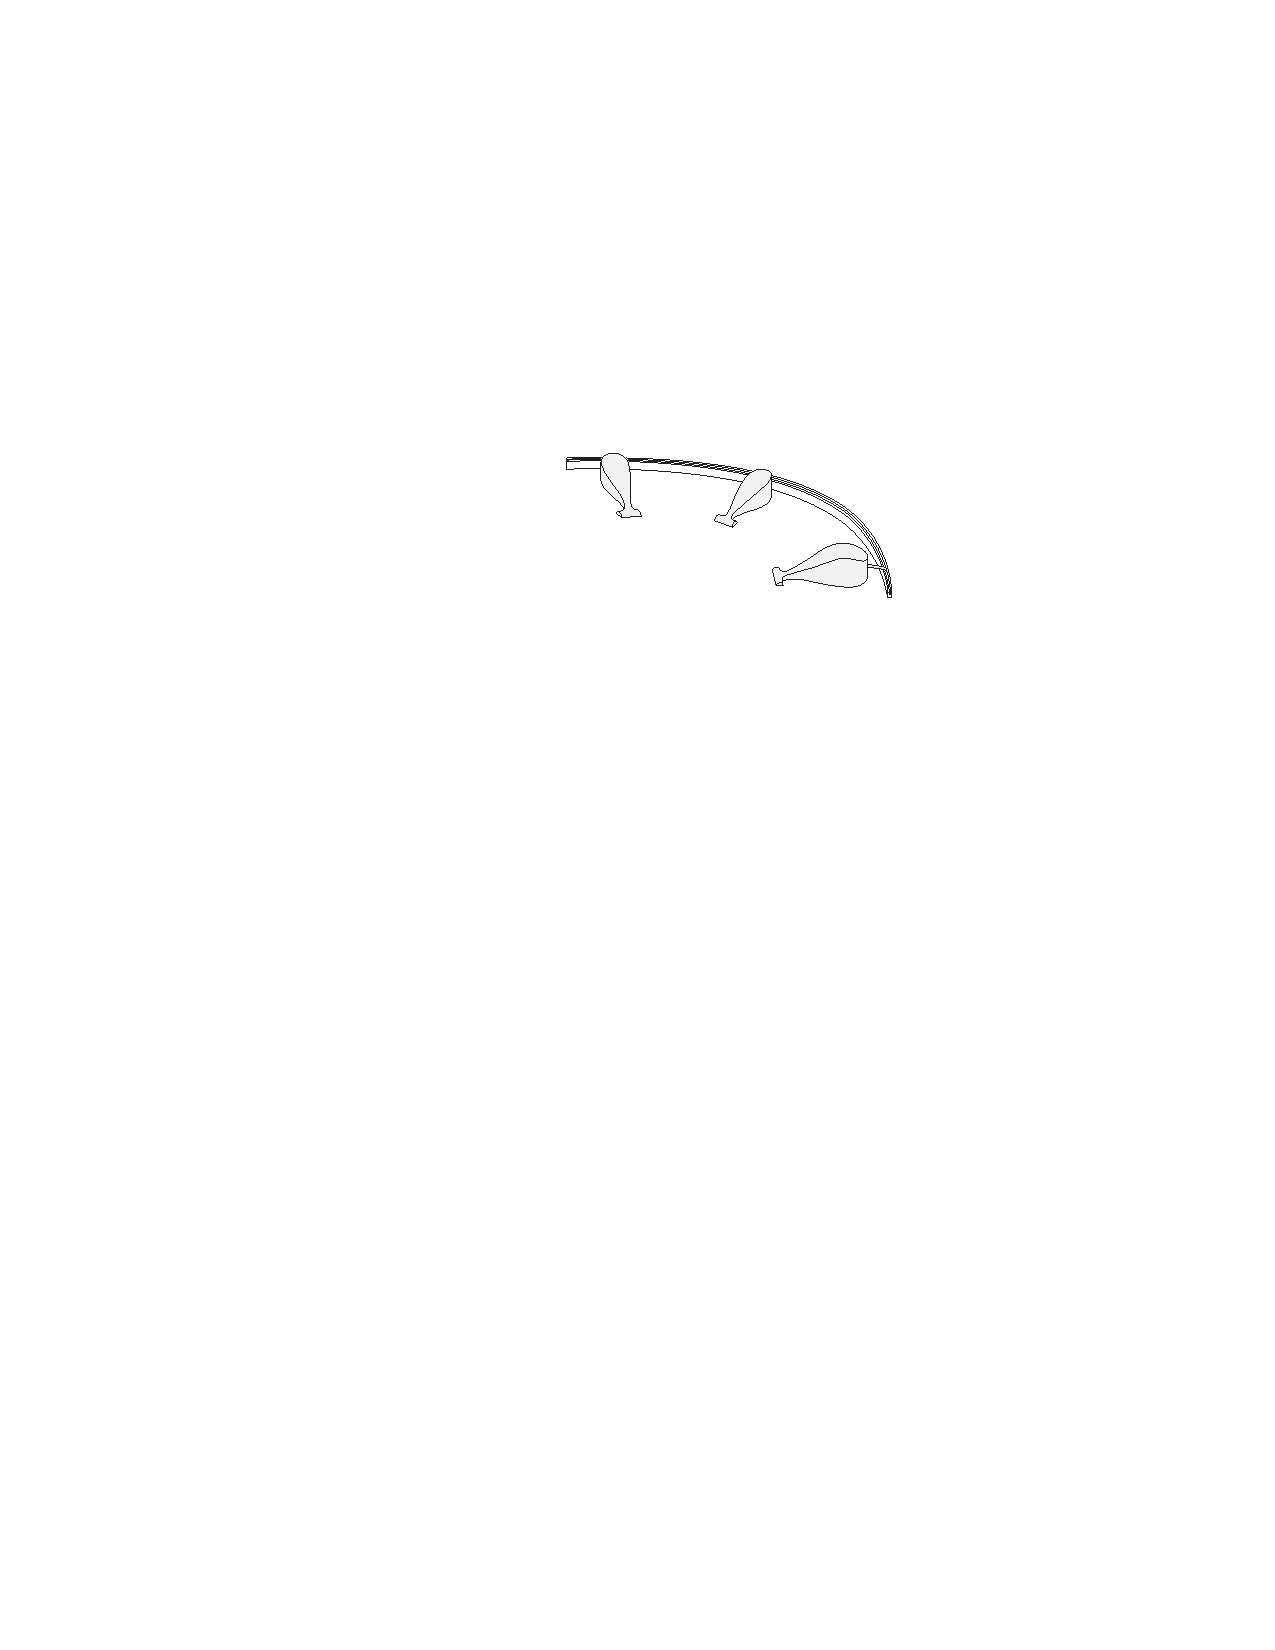
\includegraphics[height=3cm]{Images/Capitulo8/drafting_spline.pdf}
    } \hfill
    \subfloat[\label{fig:inter3}]{
    \begin{tikzpicture}[scale=1.4]
        \draw[-Stealth,thick] (-0.15,0) -- (3,0) node[above left, yshift=2pt] {$x$};
        \draw[-Stealth,thick] (0,-0.15) -- (0,2) node[below right, xshift=2pt] {$y$};
        \draw[gray, domain=0.25:2.9, samples=100] plot(\x,{0.5*(\x - 2)^3 + (\x - 2)^2 + 0.5});
        \filldraw (0.5,{0.5*(0.5 - 2)^3 + (0.5 - 2)^2 + 0.5}) circle (1.5pt);
        \filldraw (0.9,{0.5*(0.9 - 2)^3 + (0.9 - 2)^2 + 0.5}) circle (1.5pt);
        \filldraw (1.3,{0.5*(1.3 - 2)^3 + (1.3 - 2)^2 + 0.5}) circle (1.5pt);
        \filldraw (1.7,{0.5*(1.7 - 2)^3 + (1.7 - 2)^2 + 0.5}) circle (1.5pt);
        \filldraw (2.1,{0.5*(2.1 - 2)^3 + (2.1 - 2)^2 + 0.5}) circle (1.5pt);
        \filldraw (2.5,{0.5*(2.5 - 2)^3 + (2.5 - 2)^2 + 0.5}) circle (1.5pt);
        \filldraw (2.8,{0.5*(2.8 - 2)^3 + (2.8 - 2)^2 + 0.5}) circle (1.5pt);
    \end{tikzpicture}
    }
    \caption{Ejemplos de curvas de interpolación}
    \label{fig:enter-label}
\end{figure*}

\subsection*{Planteamiento del problema}

Supongamos que se nos dan $n$ puntos en el plano $xy$,
$$(x_1, y_1), (x_2, y_2), \dots, (x_n, y_n)$$
que deseamos interpolar con una curva “bien comportada” (figura \ref{fig:bienc}). Para mayor comodidad, tomamos los puntos equiespaciados en la dirección $x$, aunque nuestros resultados se pueden extender fácilmente al caso de puntos desigualmente espaciados. Si tomamos la distancia común entre las coordenadas $x$ de los puntos como $h$, entonces tenemos
$$x_2-x_1=x_3-x_2=\cdots=x_n-x_{n-1}=h$$
Sea $y = S(x)$, $x_1 \leq x \leq x_n$, la curva de interpolación que buscamos. Supondremos que esta curva describe el desplazamiento de una regla flexible que interpola los $n$ puntos cuando los pesos que sujetan la regla se sitúan precisamente en los $n$ puntos. Se sabe, por la teoría de vigas lineales, que para pequeños desplazamientos, la cuarta derivada del desplazamiento de una viga es cero a lo largo de cualquier intervalo del eje $x$ que no contenga fuerzas externas actuando sobre la viga. Si tratamos nuestra regla flexible como una viga delgada y comprendemos que las únicas fuerzas externas actuando sobre ella provienen de los pesos en los $n$ puntos especificados, entonces se sigue que
$$S^{(4)}(x) \equiv 0$$
para valores de $x$ que se encuentran en los $n-1$ intervalos abiertos
$$(x_1, x_2), (x_2, x_3), \dots , (x_{n-1}, x_n)$$
entre los $n$ puntos.
\begin{figure}[h!]
    \centering
    \includegraphics[page=4]{Images/Capitulo8/figurasC8.pdf}
    \caption{}
    \label{fig:bienc}
\end{figure}

También necesitamos el resultado de la teoría de vigas lineales que establece que, para una viga sujeta únicamente a fuerzas externas, el desplazamiento debe tener dos derivadas continuas. En el caso de la curva interpolante $y = S(x)$ construida con la regla flexible, esto significa que $S(x)$, $S′(x)$ y $S′′(x)$ deben ser continuas para $x_1 \leq x \leq x_n$.

La condición de que $S′′(x)$ sea continua es lo que hace que una regla flexible produzca una curva agradable, ya que resulta en una curvatura continua. El ojo puede percibir cambios bruscos en la curvatura, es decir, discontinuidades en $S′′(x)$, pero los cambios bruscos en derivadas de orden superior no son discernibles. Por lo tanto, la condición de que $S′′(x)$ sea continua es el requisito mínimo para que la curva interpolante sea perceptible como una curva suave única, en lugar de una serie de curvas separadas unidas.

Para determinar la forma matemática de la función $S(x)$, observamos que, dado que $S^{(4)}(x) \equiv 0$ en los intervalos entre los $n$ puntos especificados, se sigue que al resolver esta ecuación repetidamente, $S(x)$ debe ser un polinomio cúbico en $x$ en cada uno de esos intervalos. Sin embargo, en general, $S(x)$ será un polinomio cúbico diferente en cada intervalo, por lo que $S(x)$ debe tener la forma
\begin{equation}
    S(x) = \begin{cases}
        \begin{aligned}
            & S_1(x), & x_1 & \leq x \leq x_2 \\
            & S_2(x), & x_2 & \leq x \leq x_3 \\
            & \phantom{SS} \vdots & & \;\quad \vdots \\
            & S_{n-1}(x), & x_{n-1} & \leq x \leq x_n
        \end{aligned}
    \end{cases} \label{eq:S_interpola}
\end{equation}
donde $S_1(x)$, $S_2(x)$, $\dots$, $S_{n-1}(x)$ son polinomios cúbicos. Para mayor comodidad, los escribiremos de la forma
\begin{equation}
    \begin{aligned}
        S_1(x) & = a_1(x - x_1)^3 + b_1(x - x_1)^2 + c_1(x - x_1) + d_1, & x_1 & \leq x \leq x_2 \\
        S_2(x) & = a_2(x - x_2)^3 + b_2(x - x_2)^2 + c_2(x - x_2) + d_2, & x_2 & \leq x \leq x_3 \\
        & \vdots & & \\
        S_{n-1}(x) & = a_{n-1}(x - x_{n-1})^3 + b_{n-1}(x - x_{n-1})^2 & & \\
        & \hspace{3.25cm} + c_{n-1}(x - x_{n-1}) + d_{n-1}, & x_{n-1} & \leq x \leq x_n
    \end{aligned} \label{eq:S_interpola1}
\end{equation}

\newpage

Los coeficientes $a_i$, $b_i$, $c_i$ y $d_i$ constituyen un total de $4n - 4$ coeficientes, los cuales debemos determinar para definir completamente la función $S(x)$. Para lograrlo, seleccionamos estos coeficientes de manera que $S(x)$ interpole los $n$ puntos dados en el plano y, además, garantice que $S(x)$, junto con sus derivadas primera y segunda, sean continuas en todo el dominio. Estas condiciones aseguran una transición suave entre los segmentos polinómicos, lo que da lugar a la curva de interpolación conocida como \emph{spline cúbico}.

\subsection*{Derivación de la fórmula de un spline cúbico}

De las ecuaciones \eqref{eq:S_interpola} y \eqref{eq:S_interpola1}, tenemos que
\begin{align*}
    S(x) & = S_1(x) = a_1(x - x_1)^3 + b_1(x - x_1)^2 + c_1(x - x_1) + d_1, & x_1 & \leq x \leq x_2 \\
    S(x) & = S_2(x) = a_2(x - x_2)^3 + b_2(x - x_2)^2 + c_2(x - x_2) + d_2, & x_2 & \leq x \leq x_3 \\
    & \vdots & & \\
    S(x) & = S_{n-1}(x) = a_{n-1}(x - x_{n-1})^3 + b_{n-1}(x - x_{n-1})^2 & & \\
    & \hspace{4.5cm} + c_{n-1}(x - x_{n-1}) + d_{n-1}, & x_{n-1} & \leq x \leq x_n
\end{align*}
Primero, derivando la expresión \eqref{eq:S_interpola}, es decir, derivando cada polinomio anterior, se sigue que
\begin{equation}
    \begin{aligned}
        S'_1(x) & = 3a_1(x - x_1)^2 + 2b_1(x - x_1) + c_1, & x_1 & \leq x \leq x_2 \\
        S'_2(x) & = 3a_2(x - x_2)^2 + 2b_2(x - x_2) + c_2, & x_2 & \leq x \leq x_3 \\
        & \vdots & & \\
        S'_{n-1}(x) & = 3a_{n-1}(x - x_{n-1})^2 + 2b_{n-1}(x - x_{n-1}) + c_{n-1}, & x_{n-1} & \leq x \leq x_n
    \end{aligned}
\end{equation}
y derivando nuevamente, obtenemos que
\begin{align*}
    S''_1(x) & = 6a_1(x - x_1) + 2b_1, & x_1 & \leq x \leq x_2 \\
    S''_2(x) & = 6a_2(x - x_2) + 2b_2, & x_2 & \leq x \leq x_3 \\
    & \vdots & & \\
    S''_{n-1}(x) & = 6a_{n-1}(x - x_{n-1}) + 2b_{n-1}, & x_{n-1} & \leq x \leq x_n
\end{align*}
Ahora utilizaremos estas ecuaciones y las cuatro propiedades de los splines cúbicos que se indican a continuación para expresar los coeficientes desconocidos $a_i$, $b_i$, $c_i$, $d_i$ con $i = 1, 2, \dots, n - 1$, en términos de los valores conocidos $y_1$, $y_2$, $\dots$, $y_n$, lo que nos permitirá construir explícitamente la curva de interpolación deseada.

\begin{tcolorbox}[
        arc=0mm, 
        bottomtitle=0.5mm,
        boxrule=0mm,
        colbacktitle=black!10!white, 
        coltitle=black,
        left=2.5mm,
        leftrule=1mm,
        right=3.5mm,
        title={$S(x)$ interpola los puntos $(x_i, y_i)$ con $i = 1, 2, \dots, n$.},
        toptitle=0.75mm,
        colframe=black!30!white,
    ]
    Debido a que $S(x)$ interpola los puntos $(x_i, y_i)$, con $i = 1, 2, \dots, n$, tenemos
    \begin{equation}
        S(x_1) = y_1, S(x_2) = y_2, \dots, S(x_n) = y_n \label{YQUJAJAJAJAJJA}
    \end{equation}
    De las primera $n - 1$ de estas ecuaciones y \eqref{eq:S_interpola}, obtenemos
    \begin{equation}
        \begin{aligned}
            d_1 & = y_1 \\
            d_2 & = y_2 \\
            \vdots & \\
            d_{n-1} & = y_{n-1}
        \end{aligned} \label{UAJAJJAUAUHVCFATQHH}
    \end{equation}
    De la última ecuación en \eqref{YQUJAJAJAJAJJA}, la última ecuación en \eqref{eq:S_interpola}, y el hecho de que $x_n - x_{n-1} = h$, obtenemos
    \begin{equation}
        a_{n-1}h^3 + b_{n-1}h^2 + c_{n-1}h + d_{n-1} = y_n \label{UAJAJAHHCCFGYYQUYQHUU}
    \end{equation}
\end{tcolorbox}

\newpage

\begin{tcolorbox}[
        arc=0mm, 
        bottomtitle=0.5mm,
        boxrule=0mm,
        colbacktitle=black!10!white, 
        coltitle=black,
        left=2.5mm,
        leftrule=1mm,
        right=3.5mm,
        title={$S(x)$ es continua en $[x_1, x_n]$.},
        toptitle=0.75mm,
        colframe=black!30!white,
    ]
    Debido a que $S(x)$ es continuo para $x_1 \leq x \leq x_n$, se deduce que en cada punto $x_i$ en el conjunto $x_2$, $x_3$, $\dots$, $x_{n-1}$ debemos tener
    \begin{equation}
        S_{i-1}(x_i) = S_i(x_i), \quad i = 2, 3, \dots, n-1 \label{JAJAJAJJAJAVHHGGGQ}
    \end{equation}
    De lo contrario, las gráficas de $S_{i-1}(x)$ y $S_i(x)$ no se unirían para formar una curva continua en $x_i$. Cuando aplicamos la propiedad de interpolación $S_i(x_i) = y_i$, se sigue de \eqref{JAJAJAJJAJAVHHGGGQ} que $S_{i-1}(x_i) = y_i$ donde $i = 2, 3, \dots, n-1$, o de \eqref{eq:S_interpola} que
    \begin{equation}
        \begin{aligned}
            a_1h^3 + b_1h^2 + c_1h + d_1 & = y_2 \\
            a_2h^3 + b_2h^2 + c_2h + d_2 & = y_3 \\
            & \vdots \\
            a_{n-2}h^3 + b_{n-2}h^2 + c_{n-2}h + d_{n-2} & = y_{n-1}
        \end{aligned} \label{UAUAJAHCCGTTQRTQHCCTAT}
    \end{equation}
\end{tcolorbox}

\begin{tcolorbox}[
        arc=0mm, 
        bottomtitle=0.5mm,
        boxrule=0mm,
        colbacktitle=black!10!white, 
        coltitle=black,
        left=2.5mm,
        leftrule=1mm,
        right=3.5mm,
        title={$S'(x)$ es continua en $[x_1, x_n]$.},
        toptitle=0.75mm,
        colframe=black!30!white,
    ]
    Debido a que $S'(x)$ es continuo para $x_1 \leq x \leq x_n$, se deduce que
    $$S'_{i-1}(x_i) = S'_i(x_i), \quad i = 2, 3, \dots, n-1$$
    es decir
    \begin{equation}
        \begin{aligned}
            3a_1h^2 + 2b_1h + c_1 & = c_2 \\
            3a_2h^2 + 2b_2h + c_2 & = c_3 \\
            & \vdots \\
            3a_{n-2}h^2 + 2b_{n-2}h + c_{n-2} & = c_{n-1}
        \end{aligned} \label{HAJAHAHCCFGYYYAGQTTQYQHHA}
    \end{equation}
\end{tcolorbox}

\begin{tcolorbox}[
        arc=0mm, 
        bottomtitle=0.5mm,
        boxrule=0mm,
        colbacktitle=black!10!white, 
        coltitle=black,
        left=2.5mm,
        leftrule=1mm,
        right=3.5mm,
        title={$S''(x)$ es continua en $[x_1, x_n]$.},
        toptitle=0.75mm,
        colframe=black!30!white,
    ]
    Debido a que $S''(x)$ es continuo para $x_1 \leq x \leq x_n$, se deduce que
    $$S''_{i-1}(x_i) = S''_i(x_i), \quad i = 2, 3, \dots, n-1$$
    es decir
    \begin{equation}
        \begin{aligned}
            6a_1h + 2b_1 & = 2b_2 \\
            6a_2h + 2b_2 & = 2b_3 \\
            & \vdots \\
            6a_{n-2}h + 2b_{n-2} & = 2b_{n-1}
        \end{aligned} \label{YAYACCXFTQTRQRTQZFGTA}
    \end{equation}
\end{tcolorbox}

Las ecuaciones \eqref{UAJAJJAUAUHVCFATQHH}, \eqref{UAJAJAHHCCFGYYQUYQHUU}, \eqref{UAUAJAHCCGTTQRTQHCCTAT}, \eqref{HAJAHAHCCFGYYYAGQTTQYQHHA} y \eqref{YAYACCXFTQTRQRTQZFGTA} constituyen un sistema de $4n - 6$ ecuaciones lineales con $4n - 4$ coeficientes desconocidos $a_i$, $b_i$, $c_i$, $d_i$ con $i = 1, 2, \dots, n-1$. Por lo tanto, necesitamos dos ecuaciones más para determinar estos coeficientes de manera única. Sin embargo, antes de obtener estas ecuaciones adicionales, podemos simplificar nuestro sistema existente expresando las incógnitas $a_i$, $b_i$, $c_i$ y $d_i$ en términos de nuevas cantidades desconocidas:
$$M_1 = S''(x_1), M_2 = S''(x_2), \dots, M_n = S''(x_n)$$
y las cantidades conocidas $y_1$, $y_2$, $\dots$, $y_n$. Es decir,
\begin{align*}
    M_1 & = 2b_1 \\
    M_2 & = 2b_2 \\
    & \vdots \\
    M_{n-1} & = 2b_{n-1}
\end{align*}\newpage\noindent
así que
$$b_1 = \frac{1}{2}M_1, b_2 = \frac{1}{2}M_2, \dots, b_{n-1} = \frac{1}{2}M_{n-1}$$
Además, sabemos de \eqref{UAJAJJAUAUHVCFATQHH} que
$$d_1 = y_1, d_2 = y_2, \dots, d_{n-1} = y_{n-1}$$
Dejamos como ejercicio al lector derivar las expresiones de los $a_i$ y $c_i$ en términos de los $M_i$ y $y_i$. El resultado final es el siguiente:
\begin{theorem}{}{splines_cubicos}
    Consideremos $n$ puntos $(x_1, y_1)$, $(x_2, y_2)$, $\dots$, $(x_n, y_n)$ donde $x_{i+1} - x_i = h$ con $i = 1, 2, \dots, n - 1$. El spline cúbico
    $$S(x) = \begin{cases}
        \begin{aligned}
            & a_1(x - x_1)^3 + b_1(x - x_1)^2 + c_1(x - x_1) + d_1, & x_1 & \leq x \leq x_2 \\
            & a_2(x - x_2)^3 + b_2(x - x_2)^2 + c_2(x - x_2) + d_2, & x_2 & \leq x \leq x_3 \\
            & \hspace{3cm} \vdots & & \\
            & a_{n-1}(x - x_{n-1})^3 + b_{n-1}(x - x_{n-1})^2 & & \\
            & \hspace{2.75cm} + c_{n-1}(x - x_{n-1}) + d_{n-1}, & x_{n-1} & \leq x \leq x_n
        \end{aligned}
    \end{cases}$$
    que interpola estos puntos tiene como coeficientes a
    \begin{equation}
        \begin{aligned}
            a_i & = \frac{M_{i+1} - M_i}{6h} \\
            b_i & = \frac{M_i}{2} \\
            c_i & = \frac{y_{i+1} - y_i}{h} - \frac{(M_{i+1} + 2M_i)h}{6} \\
            d_i & = y_i
        \end{aligned} \label{JAJAJAIIQIQUQJAHHAVGH}
    \end{equation}
    para $i = 1, 2, \dots, n - 1$, donde $M_i = S''(x_i)$ con $i = 1, 2, \dots, n$.
\end{theorem}

A partir de este resultado, vemos que las cantidades $M_1$, $M_2$, $\dots$, $M_n$ determinan de manera única el spline cúbico. Para encontrar estas cantidades, sustituimos las expresiones de $a_i$, $b_i$ y $c_i$ dadas en \eqref{JAJAJAIIQIQUQJAHHAVGH} en \eqref{HAJAHAHCCFGYYYAGQTTQYQHHA}. Después de algunas simplificaciones algebraicas, obtenemos
\begin{equation}
    \begin{aligned}
        M_1 + 4M_2 + M_3 & = \frac{6(y_1 - 2y_2 + y_3)}{h^2} \\
        M_2 + 4M_3 + M_4 & = \frac{6(y_2 - 2y_3 + y_4)}{h^2} \\
        & \vdots \\
        M_{n-2} + 4M_{n-1} + M_n & = \frac{6(y_{n-2} - 2y_{n-1} + y_n)}{h^2}
    \end{aligned} \label{JAJAHAGYATTQTTFFFQTTTTQ}
\end{equation}
o, en forma matricial,
\begin{matrizn}
    \makecell{\includegraphics[page=11]{Externalizacion/C8/MatricesC8.pdf}}
\end{matrizn}
Observemos que este es un sistema lineal de $n - 2$ ecuaciones con $n$ incógnitas dadas por $M_1$, $M_2$, $\dots$, $M_n$. Aún necesitamos dos ecuaciones adicionales para determinar estos valores de manera única, ya que hay infinitos splines cúbicos que interpolan los puntos dados. Para obtener un spline cúbico único, se requieren condiciones adicionales. A continuación, presentamos tres formas de especificarlas, resumidas en la siguiente tabla:\newpage
\begin{table*}[h!]
    \centering
    \begin{NiceTabular}{ccc}[hvlines,cell-space-top-limit=3pt,cell-space-bottom-limit=1pt]
        \CodeBefore
        \columncolor{black!20!white}{1}
        \Body
        \makecell{Spline \\ natural} & $\begin{aligned} M_1 & = 0 \\ M_n & = 0 \end{aligned}$ & \makecell{\includegraphics[page=12]{Externalizacion/C8/MatricesC8.pdf}} \\
        \makecell{Spline de \\ salida \\ parabólica} & $\begin{aligned} M_1 & = M_2 \\ M_n & = M_{n-1} \end{aligned}$ & \makecell{\includegraphics[page=13]{Externalizacion/C8/MatricesC8.pdf}} \\
        \makecell{Spline de \\ salida \\ cúbica} & $\begin{aligned} M_1 & = 2M_2 - M_3 \\ M_n & = 2M_{n-1} - M_{n-2} \end{aligned}$ & \makecell{\includegraphics[page=14]{Externalizacion/C8/MatricesC8.pdf}}
    \end{NiceTabular}
    \caption{Condiciones adicionales para la unicidad del spline cúbico}
\end{table*}\vspace{0.4cm}

\noindent Es decir, en el spline natural, la segunda derivada del spline es cero en los extremos; en el spline de salida parabólica, el spline se reduce a una curva parabólica en los primeros y últimos intervalos; y en el spline de salida cúbica, el spline es una única curva cúbica en los dos primeros y los dos últimos intervalos.

\subsection*{El spline natural}

Las dos condiciones matemáticas más simples que podemos imponer son
$$M_1 = M_n = 0$$
Estas condiciones, junto con \eqref{JAJAHAGYATTQTTFFFQTTTTQ}, resultan en un sistema lineal de $n \times n$ para $M_1$, $M_2$, $\dots$, $M_n$, que se puede escribir en forma matricial como
\begin{matrizn}
    \makecell{\includegraphics[page=15]{Externalizacion/C8/MatricesC8.pdf}}
\end{matrizn}
Para cálculos numéricos, es más conveniente eliminar $M_1$ y $M_n$ de este sistema y escribir
\begin{matrizn}
    \makecell{\includegraphics[page=16]{Externalizacion/C8/MatricesC8.pdf}}
\end{matrizn}
junto con
\begin{align}
    M_1 & = 0 \label{UAJAJAJUAHGGGQGQGA} \\
    M_2 & = 0 \label{JAJJAJAJAJABSJSIPP}
\end{align}\newpage\noindent
Así, el sistema lineal de $(n - 2) \times (n - 2)$ puede resolverse para los $n - 2$ coeficientes $M_2$, $M_3$, $\dots$, $M_{n-1}$, y $M_1$ y $M_n$ están determinados mediante \eqref{UAJAJAJUAHGGGQGQGA} y \eqref{JAJJAJAJAJABSJSIPP}.

Físicamente, el spline natural resulta cuando los extremos de una regla flexible se extienden libremente más allá de los puntos interpolados sin restricción. Las porciones finales del spline fuera de los puntos interpolados caerán en trayectorias de líneas rectas, lo que hace que $S''(x)$ se anule en los extremos $x_1$ y $x_n$, y resultando en las condiciones matemáticas $M_1 = M_n = 0$.

El spline natural tiende a aplanar la curva interpolante en los extremos, lo cual puede ser indeseable. Por supuesto, si se requiere que $S''(x)$ se anule en los extremos, entonces se debe usar el spline natural.

\subsection*{El spline de salida parabólica}

Las dos restricciones adicionales impuestas para este tipo de spline son
\begin{align}
    M_1 & = M_2 \label{UAUAJAJJAJAVAHAGQVAHAH} \\
    M_n & = M_{n-1} \label{JAJAJAUAUJAYAYQYQHGAJ}
\end{align}
Si utilizamos las dos ecuaciones anteriores para eliminar $M_1$ y $M_n$ de \eqref{JAJAHAGYATTQTTFFFQTTTTQ}, obtenemos el sistema lineal de $(n - 2) \times (n - 2)$
\begin{matrizn}
    \makecell{\includegraphics[page=17]{Externalizacion/C8/MatricesC8.pdf}}
\end{matrizn}
para $M_2$, $M_3$, $\dots$, $M_{n-1}$. Una vez que se han determinado estos $n - 2$ valores, $M_1$ y $M_n$ se determinan a partir de \eqref{UAUAJAJJAJAVAHAGQVAHAH} y \eqref{JAJAJAUAUJAYAYQYQHGAJ}. De \eqref{JAJAJAIIQIQUQJAHHAVGH}, si $M_1 = M_2$, entonces $a_1 = 0$, y si $M_n = M_{n-1}$, entonces $a_{n-1} = 0$. Así, en \eqref{eq:S_interpola}, no hay términos cúbicos en los intervalos $[x_1, x_2]$ y $[x_{n-1}, x_n]$, por lo que el spline de salida parabólica se reduce a una curva parabólica en estos extremos.

\subsection*{El spline de salida cúbica}

Para este tipo de spline, imponemos las siguientes dos condiciones adicionales
\begin{align}
    M_1 & = 2M_2 - M_3 \label{JAJAJJAJAJQJQHCVAHAJ} \\
    M_n & = 2M_{n-1} - M_2 \label{JAJAJAJJAJAAJJAJABAJ}
\end{align}
Usando estas dos ecuaciones para eliminar $M_1$ y $M_n$ de \eqref{JAJAHAGYATTQTTFFFQTTTTQ}, resulta en el siguiente sistema lineal de $(n - 2) \times (n - 2)$ para $M_2$, $M_3$, $\dots$, $M_{n-1}$:
\begin{matrizn}
    \makecell{\includegraphics[page=18]{Externalizacion/C8/MatricesC8.pdf}}
\end{matrizn}
Después de resolver este sistema lineal para $M_2$, $M_3$, $\dots$, $M_{n-1}$, podemos usar \eqref{JAJAJJAJAJQJQHCVAHAJ} y \eqref{JAJAJAJJAJAAJJAJABAJ} para determinar $M_1$ y $M_n$.

Si reescribimos \eqref{JAJAJJAJAJQJQHCVAHAJ} como
$$M_2 - M_1 = M_3 - M_2$$\newpage\noindent
se sigue de \eqref{JAJAJAIIQIQUQJAHHAVGH} que $a_1 = a_2$. Dado que $S'''(x) = 6a_1$ en $[x_1, x_2]$ y $S'''(x) = 6a_2$ en $[x_2, x_3]$, vemos que $S'''(x)$ es constante sobre todo el intervalo $[x_1, x_3]$. En consecuencia, $S(x)$ consiste en una única curva cúbica sobre el intervalo $[x_1, x_3]$ en lugar de dos curvas cúbicas diferentes unidas en $x_2$. Un análisis similar muestra que $S(x)$ consiste en una única curva cúbica sobre los últimos dos intervalos.

Mientras que el spline natural tiende a aplanar la curva interpolante en los extremos, el spline de salida cúbica tiene el efecto contrario, generando mayor curvatura en los extremos. Si ninguno de estos comportamientos es deseado, el spline de salida parabólica ofrece un equilibrio intermedio.

\begin{examplebox}{}{splinee1}
    Es bien sabido que la densidad del agua alcanza un máximo a una temperatura ligeramente superior a la de congelación. La tabla \ref{tab:aguaa}, tomada del \emph{Handbook of Chemistry and Physics} (CRC Press, 2009), proporciona la densidad del agua en gramos por centímetro cúbico para cinco temperaturas igualmente espaciadas desde $-10$º$\mathrm{C}$ hasta $30$º$\mathrm{C}$. Interpolaremos estas cinco mediciones de temperatura y densidad utilizando un \emph{spline} parábólico con final ajustado (\emph{runout spline}) e intentaremos encontrar la densidad máxima del agua en este rango al determinar el valor máximo de este \emph{spline} cúbico. En los ejercicios, se le solicita realizar cálculos similares utilizando un \emph{spline} natural y un \emph{spline} cúbico con final ajustado para interpolar los puntos de datos.
    \begin{center}
        \begin{NiceTabular}{ccc}[hvlines,cell-space-limits=3pt]
            \cellcolor{black!20!white}{Temperatura (º$\mathrm{C}$)} & \cellcolor{black!20!white}{Densidad ($\mathrm{g}/\mathrm{cm}^3$)} \\
            \makecell[r]{$-10$ \\ $0$ \\ $10$ \\ $20$ \\ $30$} & \makecell[r]{$0.99815$ \\ $0.99987$ \\ $0.99973$ \\ $0.99823$ \\ $0.99567$}
        \end{NiceTabular}
        \captionof{table}{} \label{tab:aguaa}
    \end{center}
    Vamos a interpolar estas cinco mediciones de temperatura-densidad con un spline de salida parabólica y trataremos de encontrar la densidad máxima del agua en este rango hallando el valor máximo en este spline cúbico. Sean
    \begin{align*}
        x_1 & = -10 & y_1 & = 0.99815 \\
        x_2 & = 0 & y_2 & = 0.99987 \\
        x_3 & = 10 & y_3 & = 0.99973 \\
        x_4 & = 20 & y_4 & = 0.99823 \\
        x_5 & = 30 & y_5 & = 0.99567
    \end{align*}
    entonces
    \begin{align*}
        \frac{6(y_1 - 2y_2 + y_3)}{h^2} & = \frac{6\big(0.99815 - 2(0.99987) + 0.99973\big)}{10^2} = -0.0001116 \\
        \frac{6(y_2 - 2y_3 + y_4)}{h^2} & = \frac{6\big(0.99987 - 2(0.99973) + 0.99823\big)}{10^2} = -0.0000816 \\
        \frac{6(y_3 - 2y_4 + y_5)}{h^2} & = \frac{6\big(0.99973 - 2(0.99823) + 0.99567\big)}{10^2} = -0.0000636
    \end{align*}
    y el sistema lineal para el spline de salida parabólica se convierte en
    \begin{matrizn}
        \makecell{\includegraphics[page=19]{Externalizacion/C8/MatricesC8.pdf}}
    \end{matrizn}
    Al resolver este sistema, da como resultado
    $$M_2 = -0.00001973, \qquad M_3 = -0.00001293, \qquad M_4 = -0.00001013$$
    De \eqref{UAUAJAJJAJAVAHAGQVAHAH} y \eqref{JAJAJAUAUJAYAYQYQHGAJ}, tenemos que
    \begin{align*}
        M_1 & = M_2 = -0.00001973 \\
        M_5 & = M_4 = -0.00001013
    \end{align*}\newpage
    Al resolver para los $a_i$, $b_i$, $c_i$ y $d_i$ en \eqref{JAJAHAGYATTQTTFFFQTTTTQ}, obtenemos la siguiente expresión para el spline de terminación parabólica interpolante:
    $$\hspace{-3.5cm}S(x) = \begin{cases}
        \begin{aligned}
            -0.00000987(x + 10)^2 + 0.002707(x + 10) + 0.99815, & & -10 & \leq x \leq 0 \\
            0.00000113(x - 0)^3 - 0.00000987(x - 0)^2 + 0.000733(x - 0) + 0.99987, & & 0 & \leq x \leq 10 \\
            0.00000047(x - 10)^3 - 0.00000647(x - 10)^2 - 0.000900(x - 10) + 0.99973, & & 10 & \leq x \leq 20 \\
            - 0.00000507(x - 20)^2 - 0.002053(x - 20) + 0.99823, & & 10 & \leq x \leq 20
        \end{aligned}
    \end{cases}$$
    Este spline se muestra en la siguiente figura:
    \begin{center}
        \includegraphics[page=5]{Images/Capitulo8/figurasC8.pdf}
    \end{center}
    En dicha figura, vemos que el máximo se alcanza en el intervalo $[0, 10]$. Para encontrar este máximo, igualamos $S'(x)$ a cero en el intervalo $[0, 10]$:
    $$S'(x) = 0.000000339x^2 - 0.0001974x + 0.0000733 = 0$$
    Con tres cifras significativas, la raíz de esta ecuación cuadrática en el intervalo $[0, 10]$ es $x = 3.99$, y para este valor de $x$, $S(3.99) = 1.00001$. Así, según nuestra estimación interpolada, la densidad máxima del agua es $1.00001$ $\mathrm{g}/\mathrm{cm}^3$ alcanzada a $3.99$º$\mathrm{C}$. Esto concuerda bien con la densidad máxima experimental de $1.00000$ $\mathrm{g}/\mathrm{cm}^3$ alcanzada a $3.98$º$\mathrm{C}$.
\end{examplebox}

En conclusión, además de producir excelentes curvas de interpolación, los splines cúbicos y sus generalizaciones son útiles para la integración y diferenciación numérica, para la solución numérica de ecuaciones diferenciales e integrales, y en la teoría de la optimización.

\section{Cadenas de Markov}\label{sec:cadMarkov}

Supongamos que un sistema físico o matemático atraviesa un proceso de cambio de tal manera que en cualquier momento puede ocupar uno de un número finito de estados. Por ejemplo, el clima en una ciudad determinada podría estar en uno de tres posibles estados: soleado, nublado o lluvioso. O imaginemos que un individuo podría estar en uno de cuatro posibles estados emocionales: feliz, triste, enojado o aprensivo. Supongamos que tal sistema cambia con el tiempo de un estado a otro y que en momentos programados se observa el estado del sistema. Si el estado del sistema no puede predecirse con certeza, pero las probabilidades de los posibles estados dependen únicamente del estado previo, el proceso se denomina \emph{cadena de Markov} o \emph{proceso de Markov}.

\newpage

\begin{definicion}{}{}
    Si una cadena de Markov tiene $k$ posibles estados, etiquetados como $1, 2, \ldots, k$, entonces la probabilidad de que el sistema esté en el estado $i$ en una observación, después de haber estado en el estado $j$ en la observación anterior, se denota por $p_{ij}$ y se llama probabilidad de transición del estado $j$ al estado $i$. La matriz $P = \lBrack p_{ij} \rBrack$ se llama \emph{matriz de transición de la cadena de Markov}.
\end{definicion}

Por ejemplo, en una cadena de Markov de tres estados, la matriz de transición tiene la forma
\begin{nscenter}
    \makecell{\includegraphics[page=20]{Externalizacion/C8/MatricesC8.pdf}}
\end{nscenter}
En esta matriz, $p_{32}$ es la probabilidad de que el sistema cambie del estado $2$ al estado $3$, $p_{11}$ es la probabilidad de que el sistema permanezca en el estado $1$ si estaba previamente en el estado $1$, y así sucesivamente.

\begin{examplebox}{}{markov1}
    Una agencia de alquiler de coches tiene tres ubicaciones de alquiler, denominadas $1$, $2$ y $3$. Un cliente puede alquilar un coche en cualquiera de las tres ubicaciones y devolverlo a cualquiera de las tres ubicaciones. El gerente encuentra que los clientes devuelven los coches a las diversas ubicaciones según las siguientes probabilidades:
    \begin{nscenter}
        \makecell{\includegraphics[page=21]{Externalizacion/C8/MatricesC8.pdf}}
    \end{nscenter}
    Esta matriz es la matriz de transición del sistema considerado como una cadena de Markov. De esta matriz, se puede ver que la probabilidad de que un coche alquilado en la ubicación $3$ sea devuelto a la ubicación $2$ es de $0.3$, la probabilidad de que un coche alquilado en la ubicación $1$ sea devuelto a la ubicación $1$ es de $0.5$, y así sucesivamente.
\end{examplebox}

\begin{examplebox}{}{markov2}
    Al revisar los registros de donaciones, la oficina de exalumnos de una universidad descubre que el $80\%$ de sus exalumnos que contribuyen al fondo anual un año también contribuirán al siguiente año, y el $30\%$ de aquellos que no contribuyen un año contribuirán al siguiente. Esto se puede ver como una cadena de Markov con dos estados: el estado $1$ corresponde a un exalumno que dona en un año determinado, y el estado $2$ corresponde a un exalumno que no dona en ese año. La matriz de transición es
    $$P = \begin{bmatrix}
        0.80 & 0.30 \\
        0.20 & 0.70
    \end{bmatrix}$$
\end{examplebox}

En los ejemplos anteriores, las matrices de transición de las cadenas de Markov tienen la propiedad de que la suma de las entradas en cualquier columna es igual a $1$. Esto no es accidental. Si $P = \lBrack p_{ij} \rBrack$ es la matriz de transición de cualquier cadena de Markov con $k$ estados, entonces para cada $j$ debemos tener
\begin{equation}
    p_{1j} + p_{2j} + \cdots + p_{kj} = 1 \label{IAUAUAIQIOQPQOQJQCCCAHAIAIAIA}
\end{equation}
porque si el sistema está en el estado $j$ en una observación, es seguro que estará en uno de los $k$ estados posibles en la siguiente observación.

Una matriz con la propiedad \eqref{IAUAUAIQIOQPQOQJQCCCAHAIAIAIA} se llama \emph{matriz estocástica}, \emph{matriz de probabilidad} o \emph{matriz de Markov}. De la discusión anterior, se sigue que la matriz de transición para una cadena de Markov debe ser una matriz estocástica.

\newpage

En una cadena de Markov, el estado del sistema en cualquier momento de observación generalmente no puede determinarse con certeza. Lo mejor que se puede hacer normalmente es especificar probabilidades para cada uno de los estados posibles. Por ejemplo, en una cadena de Markov con tres estados, podríamos describir el estado posible del sistema en algún momento de observación mediante un vector columna
\begin{matrizn}
    \makecell{\includegraphics[page=22]{Externalizacion/C8/MatricesC8.pdf}}
\end{matrizn}
en el cual, $x_1$ es la probabilidad de que el sistema esté en el estado $1$, $x_2$ es la probabilidad de que esté en el estado $2$, $x_3$ es la probabilidad de que esté en el estado $3$, y $x_4$ es la probabilidad de que esté en el estado $4$. En general, tenemos la siguiente definición.

\begin{definicion}{}{}
    El \emph{vector de estado} para una observación de una cadena de Markov con $k$ estados es un vector columna $\mathbb{x}$, cuya $i$-ésima componente $x_i$ es la probabilidad de que el sistema esté en el estado $i$ en ese momento.
\end{definicion}

Observe que las entradas en cualquier vector de estado para una cadena de Markov son no negativas y suman $1$ (¿por qué?). Un vector columna que tiene esta propiedad se llama \emph{vector de probabilidad}.

Supongamos ahora que conocemos el vector de estado $\mathbb{x}^{(0)}$ para una cadena de Markov en alguna observación inicial. El siguiente teorema nos permitirá determinar los vectores de estado
$$\mathbb{x}^{(1)}, \mathbb{x}^{(2)}, \dots, \mathbb{x}^{(n)}, \dots$$
en los tiempos de observación subsiguientes.

\begin{theorem}{}{matrix_transition-state}
    Si $P$ es la matriz de transición de una cadena de Markov y $\mathbb{x}^{(n)}$ es el vector de estado en la $n$-ésima observación, entonces $\mathbb{x}^{(n+1)} = P \mathbb{x}^{(n)}$.
\end{theorem}

La demostración del teorema anterior recurre a conceptos avanzados de la teoría de probabilidad, los cuales exceden el alcance de esta presentación, por lo que no se incluirá aquí. Sin embargo, como consecuencia directa de este teorema, se deduce que
\begin{align*}
    \mathbb{x}^{(1)} & = P\mathbb{x}^{(0)} \\
    \mathbb{x}^{(2)} & = P\mathbb{x}^{(1)} = P^2\mathbb{x}^{(0)} \\
    \mathbb{x}^{(3)} & = P\mathbb{x}^{(2)} = P^3\mathbb{x}^{(0)} \\
    \mathbb{x}^{(4)} & = P\mathbb{x}^{(3)} = P^4\mathbb{x}^{(0)} \\
    & \vdots \\
    \mathbb{x}^{(n)} & = P\mathbb{x}^{(n-1)} = P^n\mathbb{x}^{(0)}
\end{align*}
De esta manera, el vector de estado inicial $\mathbb{x}^{(0)}$ y la matriz de transición $P$ determinan $\mathbb{x}^{(n)}$ para $n = 1, 2, \dots$.

\begin{examplebox}{}{markov3}
    La matriz de transición en el ejemplo \ref{examplebox:markov2} era
    $$P = \begin{bmatrix}
        0.8 & 0.3 \\
        0.2 & 0.7
    \end{bmatrix}$$
    Ahora construimos el probable registro futuro de donaciones de un nuevo graduado que no hizo una donación en el año inicial después de la graduación. Para tal graduado, el sistema está inicialmente en el estado $2$ con certeza, por lo que el vector de estado inicial es
    $$\mathbb{x}^{(0)} = \begin{bmatrix} 0 \\ 1 \end{bmatrix}$$\newpage
    A partir del teorema \ref{theorem:matrix_transition-state}, tenemos entonces
    \begin{align*}
        \mathbb{x}^{(1)} & = P\mathbb{x}^{(0)} = \begin{bmatrix} 0.8 & 0.3 \\ 0.2 & 0.7 \end{bmatrix} \begin{bmatrix} 0 \\ 1 \end{bmatrix} = \begin{bmatrix} 0.3 \\ 0.7 \end{bmatrix} \\
        \mathbb{x}^{(2)} & = P\mathbb{x}^{(1)} = \begin{bmatrix} 0.8 & 0.3 \\ 0.2 & 0.7 \end{bmatrix} \begin{bmatrix} 0.3 \\ 0.7 \end{bmatrix} = \begin{bmatrix} 0.45 \\ 0.55 \end{bmatrix} \\
        \mathbb{x}^{(3)} & = P\mathbb{x}^{(2)} = \begin{bmatrix} 0.8 & 0.3 \\ 0.2 & 0.7 \end{bmatrix} \begin{bmatrix} 0.45 \\ 0.55 \end{bmatrix} = \begin{bmatrix} 0.525 \\ 0.475 \end{bmatrix}
    \end{align*}
    Así, después de tres años, se espera que el exalumno haga una donación con una probabilidad de $0.525$. Más allá de tres años, encontramos los siguientes vectores de estado (con tres decimales):
    \begin{align*}
        \mathbb{x}^{(4)} & = \begin{bmatrix} 0.563 \\ 0.438 \end{bmatrix}, & \mathbb{x}^{(5)} & = \begin{bmatrix} 0.581 \\ 0.419 \end{bmatrix}, & \mathbb{x}^{(6)} & = \begin{bmatrix} 0.591 \\ 0.409 \end{bmatrix}, & \mathbb{x}^{(7)} & = \begin{bmatrix} 0.595 \\ 0.405 \end{bmatrix}, \\
        \mathbb{x}^{(8)} & = \begin{bmatrix} 0.598 \\ 0.402 \end{bmatrix}, & \mathbb{x}^{(9)} & = \begin{bmatrix} 0.599 \\ 0.401 \end{bmatrix}, & \mathbb{x}^{(10)} & = \begin{bmatrix} 0.599 \\ 0.401 \end{bmatrix}, & \mathbb{x}^{(11)} & = \begin{bmatrix} 0.600 \\ 0.400 \end{bmatrix}
    \end{align*}
    Para todos los $n$ mayores de $11$, tenemos
    $$\mathbb{x}^{(n)} = \begin{bmatrix} 0.600 \\ 0.400 \end{bmatrix}$$
    con tres decimales. En otras palabras, los vectores de estado convergen a un vector fijo a medida que aumenta el número de observaciones.
\end{examplebox}

\begin{examplebox}{}{markov4}
    La matriz de transición en el ejemplo \ref{examplebox:markov1} era
    \begin{matrizn}
        \makecell{\includegraphics[page=23]{Externalizacion/C8/MatricesC8.pdf}}
    \end{matrizn}
    Si un auto se alquila inicialmente desde la ubicación $2$, entonces el vector de estado inicial es
    \begin{matrizn}
        \makecell{\includegraphics[page=24]{Externalizacion/C8/MatricesC8.pdf}}
    \end{matrizn}
    Usando este vector y el teorema \ref{theorem:matrix_transition-state}, se obtienen los siguientes vectores de estado que se enumeran en la siguiente tabla:
    \begin{adjustwidth}{-7.5cm}{-2cm}
        \vspace{0.3cm}\centering
        \begin{NiceTabular}{ccccccccccccc}[vlines,cell-space-limits=4pt]
            \CodeBefore
            \rowcolor{black!20!white}{1,2}
            \columncolor{black!20!white}{1}
            \Body
            \hline
            \Block{2-1}{\diagbox{\raisebox{4pt}{\hspace*{0.1cm} $\mathbb{x}^{(n)}$}}{\raisebox{-0.4cm}{$n$\hspace{0.3cm}}}} & \Block{2-1}{$0$} & \Block{2-1}{$1$} & \Block{2-1}{$2$} & \Block{2-1}{$3$} & \Block{2-1}{$4$} & \Block{2-1}{$5$} & \Block{2-1}{$6$} & \Block{2-1}{$7$} & \Block{2-1}{$8$} & \Block{2-1}{$9$} & \Block{2-1}{$10$} & \Block{2-1}{$11$}\\
            \hspace{1.5cm} & \\
            \hline
            $x_1^{(n)}$ & $0$ & $0.300$ & $0.400$ & $0.477$ & $0.511$ & $0.533$ & $0.544$ & $0.550$ & $0.553$ & $0.555$ & $0.556$ & $0.557$ \\
            $x_2^{(n)}$ & $1$ & $0.200$ & $0.370$ & $0.252$ & $0.261$ & $0.240$ & $0.238$ & $0.233$ & $0.232$ & $0.231$ & $0.230$ & $0.230$ \\
            $x_3^{(n)}$ & $0$ & $0.500$ & $0.230$ & $0.271$ & $0.228$ & $0.227$ & $0.219$ & $0.217$ & $0.215$ & $0.214$ & $0.214$ & $0.213$ \\
            \hline
        \end{NiceTabular} \vspace{0.3cm}
    \end{adjustwidth}
    Para todos los valores de $n$ mayores a $11$, todos los vectores de estado son iguales a $\mathbb{x}^{(11)}$ con tres decimales. Esto indica que el sistema ha alcanzado un estado estable, en el cual las probabilidades de transición ya no generan cambios significativos en la distribución del estado. Se deben observar dos aspectos clave en este ejemplo. Primero, no era necesario conocer la duración exacta del tiempo que un cliente mantiene el coche. En otras palabras, en un proceso de Markov, el intervalo de tiempo entre observaciones no necesita ser regular, lo que lo hace útil en situaciones donde las transiciones ocurren en momentos aleatorios o no uniformes. Segundo, los vectores de estado se aproximan hacia un vector fijo a medida que $n$ aumenta. Esto sugiere que el sistema alcanza un equilibrio estacionario, lo que es una propiedad fundamental de las cadenas de Markov.
\end{examplebox}

\newpage
\sideFigure[\label{fig:police}]{\vspace{1.5cm}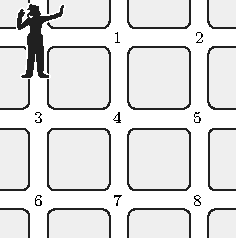
\includegraphics[width=\linewidth]{Images/Capitulo8/Police.pdf}}
\begin{examplebox}{}{markov5}
    Una oficial de tráfico está asignada a controlar el tráfico en las ocho intersecciones indicadas en la figura \ref{fig:police}. Se le instruye permanecer en cada intersección durante una hora y luego, ya sea permanecer en la misma intersección o moverse a una intersección vecina. Para evitar establecer un patrón, se le indica elegir su nueva intersección de manera aleatoria, con cada elección posible igualmente probable. Por ejemplo, si se encuentra en la intersección $5$, su próxima intersección puede ser $2$, $4$, $5$, o $8$, cada una con una probabilidad de $1/4$. Cada día, comienza en el lugar donde se detuvo el día anterior. La matriz de transición para esta cadena de Markov es:
    \begin{matrizn}
        \makecell{\includegraphics[page=25]{Externalizacion/C8/MatricesC8.pdf}}
    \end{matrizn}
    Si la oficial de tráfico comienza en la intersección $5$, sus ubicaciones probables, hora por hora, están dadas por los vectores de estado que se muestran en la tabla precedente. Para todos los valores de $n$ mayores que $22$, todos los vectores de estado son iguales a $\mathbb{x}^{(22)}$ con tres decimales. Así, al igual que en los dos primeros ejemplos, los vectores de estado se acercan a un vector fijo a medida que $n$ aumenta.
    \begin{adjustwidth}{-7.5cm}{-2cm}
        \vspace{0.3cm}\centering
        \begin{NiceTabular}{cccccccccccccc}[vlines,cell-space-limits=4pt]
            \CodeBefore
            \rowcolor{black!20!white}{1}
            \columncolor{black!20!white}{1}
            \rowcolor{black!20!white}{2}
            \Body
            \hline
            \Block{2-1}{\diagbox{\raisebox{4pt}{\hspace*{0.1cm} $\mathbb{x}^{(n)}$}}{\raisebox{-0.4cm}{$n$\hspace{0.3cm}}}} & \Block{2-1}{$0$} & \Block{2-1}{$1$} & \Block{2-1}{$2$} & \Block{2-1}{$3$} & \Block{2-1}{$4$} & \Block{2-1}{$5$} & \Block{2-1}{$\cdots$} & \Block{2-1}{$10$} & \Block{2-1}{$\cdots$} & \Block{2-1}{$15$} & \Block{2-1}{$\cdots$} & \Block{2-1}{$21$} & \Block{2-1}{$22$} \\
            \hspace{1.5cm} & \\
            \hline
            $x_1^{(n)}$ & $0$ & $0.000$ & $0.133$ & $0.116$ & $0.130$ & $0.123$ & $\cdots$ & $0.113$ & $\cdots$ & $0.109$ & $\cdots$ & $0.108$ & $0.107$ \\
            $x_2^{(n)}$ & $0$ & $0.250$ & $0.146$ & $0.163$ & $0.140$ & $0.138$ & $\cdots$ & $0.115$ & $\cdots$ & $0.109$ & $\cdots$ & $0.108$ & $0.107$ \\
            $x_3^{(n)}$ & $0$ & $0.000$ & $0.050$ & $0.039$ & $0.067$ & $0.073$ & $\cdots$ & $0.100$ & $\cdots$ & $0.106$ & $\cdots$ & $0.107$ & $0.107$ \\
            $x_4^{(n)}$ & $0$ & $0.250$ & $0.113$ & $0.187$ & $0.162$ & $0.178$ & $\cdots$ & $0.178$ & $\cdots$ & $0.179$ & $\cdots$ & $0.179$ & $0.179$ \\
            $x_5^{(n)}$ & $1$ & $0.250$ & $0.279$ & $0.190$ & $0.190$ & $0.168$ & $\cdots$ & $0.149$ & $\cdots$ & $0.144$ & $\cdots$ & $0.143$ & $0.143$ \\
            $x_6^{(n)}$ & $0$ & $0.000$ & $0.000$ & $0.050$ & $0.056$ & $0.074$ & $\cdots$ & $0.099$ & $\cdots$ & $0.105$ & $\cdots$ & $0.107$ & $0.107$ \\
            $x_7^{(n)}$ & $0$ & $0.000$ & $0.133$ & $0.104$ & $0.131$ & $0.125$ & $\cdots$ & $0.138$ & $\cdots$ & $0.142$ & $\cdots$ & $0.143$ & $0.143$ \\
            $x_8^{(n)}$ & $0$ & $0.250$ & $0.146$ & $0.152$ & $0.124$ & $0.121$ & $\cdots$ & $0.108$ & $\cdots$ & $0.107$ & $\cdots$ & $0.107$ & $0.107$ \\
            \hline
        \end{NiceTabular} \vspace{0.3cm}
    \end{adjustwidth}
\end{examplebox}

En nuestros ejemplos vimos que los vectores de estado se aproximaban a un vector fijo a medida que aumentaba el número de observaciones. Ahora nos preguntamos si los vectores de estado siempre se aproximan a un vector fijo en una cadena de Markov. Un ejemplo sencillo muestra que este no es siempre el caso.

\newpage

\begin{examplebox}{}{}
    Sean
    $$P = \begin{bmatrix}
        0 & 1 \\
        1 & 0
    \end{bmatrix} \quad \text{ y } \quad \mathbb{x}^{(0)} = \begin{bmatrix}
        1 \\
        0
    \end{bmatrix}$$
    Entonces, dado que $P^2 = I_2$ y $P^3 = P$, tenemos que
    $$\mathbb{x}^{(0)} = \mathbb{x}^{(2)} = \mathbb{x}^{(4)} = \cdots = \begin{bmatrix} 1 \\ 0 \end{bmatrix}$$
    y
    $$\mathbb{x}^{(1)} = \mathbb{x}^{(3)} = \mathbb{x}^{(5)} = \cdots = \begin{bmatrix} 0 \\ 1 \end{bmatrix}$$
    Este sistema oscila indefinidamente entre los dos vectores $\begin{bmatrix} 0 \\ 1 \end{bmatrix}$ y $\begin{bmatrix} 1 \\ 0 \end{bmatrix}$, por lo que no se aproxima a ningún vector fijo.
\end{examplebox}

No obstante, si imponemos una condición simple a la matriz de transición, podemos demostrar que se alcanza un vector de estado fijo. Esta condición se define a continuación.

\begin{definicion}{}{}
    Una matriz de transición se considera \emph{regular} si, al elevarla a alguna potencia entera, todas sus entradas son positivas.
\end{definicion}

Por lo tanto, para una matriz de transición regular $P$, existe un entero positivo $m$ tal que todas las entradas de $P^m$ son positivas. Este es el caso de las matrices de transición en los ejemplos \ref{examplebox:markov1} y \ref{examplebox:markov2} con $m = 1$. En el ejemplo \ref{examplebox:markov5}, resulta que $P^4$ tiene todas las entradas positivas. Por lo tanto, en los tres ejemplos, las matrices de transición son regulares. Esto significa que dichas matrices satisfacen una propiedad clave: cualquier estado puede alcanzarse desde cualquier otro estado después de un número finito de pasos, lo cual garantiza una conectividad total en el espacio de estados.

Una cadena de Markov con una matriz de transición regular se llama \emph{cadena de Markov regular}. Este tipo de cadenas exhibe un comportamiento especial: independientemente del estado inicial $\mathbb{x}^{(0)}$, la distribución de probabilidad del estado converge hacia un único vector de estado fijo $\mathbb{q}$ a medida que el número de pasos $n$ tiende a infinito. Este vector $\mathbb{q}$ es invariante bajo la acción de la matriz $P$, es decir, satisface $P \mathbb{q} = \mathbb{q}$.

La existencia de este vector fijo $\mathbb{q}$ es de suma importancia porque describe el comportamiento a largo plazo del sistema modelado por la cadena de Markov. Por ejemplo, en aplicaciones como redes de comunicación, procesos biológicos, o modelos económicos, este resultado permite predecir el estado estable del sistema, independientemente de su configuración inicial. Además, la unicidad y positividad de los elementos de $\mathbb{q}$ garantizan que el sistema tiene una distribución de probabilidad única en el límite, asegurando estabilidad en el análisis.

El resultado mencionado se basa en el siguiente teorema fundamental:

\begin{theorem}{}{tomarkov2}
    Si $P$ es una matriz de transición regular, entonces a medida que $n \to \infty$,
    \begin{matrizn}
        \makecell{\includegraphics[page=26]{Externalizacion/C8/MatricesC8.pdf}}
    \end{matrizn}
    donde los $q_i$ son números positivos tales que $q_1 + q_2 + \cdots + q_k = 1$.
\end{theorem}

Este teorema formaliza la idea de que, para cadenas de Markov regulares, la matriz de transición elevada a potencias suficientemente grandes se estabiliza en una forma en la que cada fila es idéntica y corresponde al vector de estado fijo $\mathbb{q}$.
\infoBulle{No demostraremos este teorema aquí. Para una demostración detallada, consulte un texto más especializado, como J. Kemeny y J. Snell, \emph{Finite Markov Chains} (New York: Springer-Verlag, 1976).}

\newpage

Consideremos
\begin{matrizn}
    \makecell{\includegraphics[page=27]{Externalizacion/C8/MatricesC8.pdf}}
\end{matrizn}
Es decir, $Q$ es una matriz de transición cuyas columnas son todas iguales al vector de probabilidad $\mathbb{q}$. $Q$ tiene la propiedad de que si $\mathbb{x}$ es cualquier vector de probabilidad, entonces
\begin{nscenter}
    \makecell{\includegraphics[page=28]{Externalizacion/C8/MatricesC8.pdf}}
\end{nscenter}
Es decir, $Q$ transforma cualquier vector de probabilidad $\mathbb{x}$ en el vector de probabilidad fijo $\mathbb{q}$. Este resultado nos lleva al siguiente teorema.

\begin{theorem}{}{tomarkov3}
    Si $P$ es una matriz de transición regular y $\mathbb{x}$ es cualquier vector de probabilidad, entonces, conforme $n \to \infty$, 
    \begin{nscenter}
        \makecell{\includegraphics[page=29]{Externalizacion/C8/MatricesC8.pdf}}
    \end{nscenter}
    donde $\mathbb{q}$ es un vector de probabilidad fijo, independiente de $n$, y cuyos componentes son todos positivos.
\end{theorem}

Este resultado se cumple ya que el teorema \ref{theorem:tomarkov2} implica que $P^n \to Q$ a medida que $n \to \infty$. Esto, a su vez, implica que $P^n\mathbb{x} \to Q\mathbb{x} = \mathbb{q}$ a medida que $n \to \infty$. Así, para una cadena de Markov regular, el sistema se aproxima a un vector de estado fijo $\mathbb{q}$. Este vector $\mathbb{q}$ se llama el \emph{vector de estado estacionario} de la cadena de Markov regular. Para sistemas con muchos estados, la forma más eficiente de calcular el vector de estado estacionario $\mathbb{q}$ es evaluar $P^n \mathbb{x}$ para un $n$ grande. Nuestros ejemplos muestran este procedimiento, garantizando la convergencia debido a la regularidad del proceso. Alternativamente, $\mathbb{q}$ puede calcularse mediante el siguiente teorema.

\begin{theorem}{}{tomarkov4}
    El vector de estado estacionario $\mathbb{q}$ de una matriz de transición regular $P$ es el único vector de probabilidad que satisface la ecuación $P \mathbb{q} = \mathbb{q}$.
\end{theorem}

Para entender esto, consideremos la identidad $PP^n = P^{n+1}$. Por el teorema \ref{theorem:tomarkov2}, tanto $P^n$ como $P^{n+1}$ convergen a $Q$ cuando $n \to \infty$, lo que implica $PQ = Q$ y, por lo tanto, $P\mathbb{q} = \mathbb{q}$. Para demostrar la unicidad de $\mathbb{q}$, supongamos que existe otro vector de probabilidad $\mathbb{r}$ con $P\mathbb{r} = \mathbb{r}$. Entonces, $P^n\mathbb{r} = \mathbb{r}$ para todo $n$. Tomando el límite cuando $n \to \infty$ y aplicando el teorema \ref{theorem:tomarkov3}, se concluye que $\mathbb{q} = \mathbb{r}$.

\newpage

La ecuación del teorema \ref{theorem:tomarkov4} también se puede expresar como un sistema lineal homogéneo
$$(I_k - P)\mathbb{q} = \mathbb{0}$$
donde tiene una solución única, el vector $\mathbb{q}$, con entradas no negativas que satisfacen la condición $q_1 + q_2 + \cdots + q_k = 1$. Podemos aplicar esta técnica para calcular los vectores de estado estacionario en nuestros ejemplos.

\begin{examplebox}{}{}
    En el ejemplo \ref{examplebox:markov2}, la matriz de transición era
    $$P = \begin{bmatrix} 
        0.8 & 0.3 \\ 
        0.2 & 0.7 
    \end{bmatrix}$$
    Entonces, el sistema lineal $(I_2 - P)\mathbb{q} = \mathbb{0}$ es
    $$\begin{bmatrix*}[r]
        0.2 & -0.3 \\
        -0.2 & 0.3
    \end{bmatrix*}\begin{bmatrix}
        q_1 \\
        q_2
    \end{bmatrix} = \begin{bmatrix}
        0 \\
        0
    \end{bmatrix}$$
    Esto lleva a la única ecuación independiente
    $$0.2q_1 - 0.3q_2 = 0$$
    o bien,
    $$q_1 = 1.5q_2$$
    Es decir, la solución general al sistema está dada por
    $$\mathbb{q} = \begin{bmatrix}
        1.5q_2 \\
        q_2
    \end{bmatrix} = q_2 \begin{bmatrix}
        1.5 \\
        1
    \end{bmatrix}$$
    Para que el vector $\mathbb{q}$ sea un vector de probabilidad, la suma de las entradas de $\mathbb{q}$ debe ser igual a $1$. Así,
    $$q_2 = \frac{1}{1.5 + 1} = 0.4$$
    Por consiguiente,
    $$\mathbb{q} = \begin{bmatrix}
        0.6 \\
        0.4
    \end{bmatrix}$$
    es el vector de estado estacionario de esta cadena de Markov regular. Esto significa que a largo plazo, el $60\%$ de los exalumnos harán una donación en un año determinado, y el $40\%$ no lo harán. Además, estos porcentajes se mantendrán constantes en el tiempo, independientemente del estado inicial de la población. Observe que esto concuerda con el resultado obtenido numéricamente en el ejemplo \ref{examplebox:markov3}.
\end{examplebox}

\begin{examplebox}{}{}
    En el ejemplo \ref{examplebox:markov1}, la matriz de transición era
    \begin{matrizn}
        \makecell{\includegraphics[page=30]{Externalizacion/C8/MatricesC8.pdf}}
    \end{matrizn}
    Así que el sistema lineal $(I_3 - P)\mathbb{q} = \mathbb{0}$ está dado por
    \begin{matrizn}
        \makecell{\includegraphics[page=31]{Externalizacion/C8/MatricesC8.pdf}}
    \end{matrizn}
    Utilizando el método de reducción de Gauss-Jordan, obtenemos que
    \begin{nscenter}
        \makecell{\includegraphics[page=32]{Externalizacion/C8/MatricesC8.pdf}}
    \end{nscenter}
    \newpage
    Por lo que el sistema lineal original es equivalente al sistema
    \begin{align*}
        q_1 & = \frac{34}{13} q_3 \\
        q_2 & = \frac{14}{13} q_3
    \end{align*}
    Es decir, la solución general al sistema está dada por
    \begin{matrizn}
        \makecell{\includegraphics[page=33]{Externalizacion/C8/MatricesC8.pdf}}
    \end{matrizn}
    Para que el vector $\mathbb{q}$ sea un vector de probabilidad, la suma de las entradas de $\mathbb{q}$ debe ser igual a $1$. Así,
    $$q_3 = \frac{1}{\dfrac{34}{13} + \dfrac{14}{13} + 1} = \frac{13}{61}$$
    Por consiguiente, el vector de estado estacionario del sistema es
    \begin{matrizn}
        \makecell{\includegraphics[page=34]{Externalizacion/C8/MatricesC8.pdf}}
    \end{matrizn}
    Esto concuerda con el resultado obtenido numéricamente en la tabla del ejemplo \ref{examplebox:markov4}. Los valores de $\mathbb{q}$ dan las probabilidades a largo plazo de que cualquier coche sea devuelto a la ubicación $1$, $2$ o $3$, respectivamente. Si la agencia de alquiler de coches tiene una flota de $1 \, 000$ coches, debería diseñar sus instalaciones de manera que haya al menos $558$ espacios en la ubicación $1$, al menos $230$ espacios en la ubicación $2$, y al menos $214$ espacios en la ubicación $3$.
\end{examplebox}

\begin{examplebox}{}{}
    Tomemos la matriz de transición del ejemplo \ref{examplebox:markov5}. No daremos los detalles de los cálculos, pero simplemente afirmaremos que la única solución del vector de probabilidad para el sistema lineal $(I_8 - P)\mathbb{q} = \mathbb{0}$ es
    \begin{matrizn}
        \makecell{\includegraphics[page=35]{Externalizacion/C8/MatricesC8.pdf}}
    \end{matrizn}
    Esto concuerda con el resultado obtenido numéricamente en la tabla del ejemplo \ref{examplebox:markov5}. Los valores de este vector indican la proporción de tiempo que la oficial de tráfico pasa en cada intersección a largo plazo, mostrando que su presencia no se distribuye de manera uniforme. En otras palabras, algunas intersecciones recibirán más atención que otras de manera natural bajo esta estrategia. Por lo tanto, si se busca que pase la misma cantidad de tiempo en todas las intersecciones, la estrategia de moverse aleatoriamente con probabilidades iguales no es adecuada. En su lugar, sería necesario diseñar una estrategia alternativa que ajuste las probabilidades de movimiento entre intersecciones para alcanzar una distribución uniforme, optimizando así el tiempo dedicado en cada una.
\end{examplebox}

\newpage

\section{Teoría de grafos}

Existen innumerables ejemplos de conjuntos finitos donde sus elementos están relacionados de alguna manera. Por ejemplo, el conjunto podría estar compuesto por personas, animales, países, empresas, equipos deportivos o ciudades. La relación entre dos elementos, $A$ y $B$, podría ser que la persona $A$ domina a la persona $B$, el animal $A$ se alimenta del animal $B$, el país $A$ apoya militarmente al país $B$, la empresa $A$ vende su producto a la empresa $B$, el equipo deportivo $A$ siempre vence al equipo deportivo $B$, o la ciudad $A$ tiene un vuelo directo a la ciudad $B$.

Ahora mostraremos cómo la teoría de \emph{grafos dirigidos} puede utilizarse para modelar matemáticamente relaciones como estas.

\subsection*{Grafos dirigidos}
\sideFigure[\label{fig:examgrafos1}]{
\includegraphics[page=6]{Images/Capitulo8/figurasC8.pdf}
}

Un grafo dirigido es un conjunto finito de elementos $\{P_1, P_2, \dots, P_n\}$ junto con una colección finita de pares ordenados $(P_i, P_j)$ de elementos distintos de este conjunto, sin repetir ningún par ordenado. Los elementos del conjunto se llaman vértices, y los pares ordenados se llaman aristas dirigidas del grafo dirigido. Usamos la notación $P_i \rightarrow P_j$ (que se lee “$P_i$ está conectado a $P_j$”) para indicar que la arista dirigida $(P_i, P_j)$ pertenece al grafo dirigido. Geométricamente, podemos visualizar un grafo dirigido (figura \ref{fig:examgrafos1}) representando los vértices como puntos en el plano y representando la arista dirigida $P_i \rightarrow P_j$ dibujando una línea o arco desde el vértice $P_i$ hasta el vértice $P_j$, con una flecha que apunta de $P_i$ a $P_j$. Si tanto $P_i \rightarrow P_j$ como $P_j \rightarrow P_i$ son ciertos (denotado $P_i \leftrightarrow P_j$), dibujamos una sola línea entre $P_i$ y $P_j$ con dos flechas apuntando en direcciones opuestas (como con $P_2$ y $P_3$ en la figura).

Como se muestra en la figura \ref{fig:examgrafos1}, un grafo dirigido puede tener componentes separadas de vértices que están conectados solo entre sí; y algunos vértices, como $P_5$, pueden no estar conectados con ningún otro vértice. Además, dado que $P_i \rightarrow P_i$ no está permitido en un grafo dirigido, un vértice no puede estar conectado consigo mismo por un solo arco que no pase por ningún otro vértice.

La figura \ref{fig:examgrafos2} muestra diagramas que representan tres ejemplos más de grafos dirigidos.
\begin{figure*}[h!]
    \centering
    \subfloat[\label{fig:examgrafos2a}]{
    \includegraphics[page=7]{Images/Capitulo8/figurasC8.pdf}
    } \hfill
    \subfloat[\label{fig:examgrafos2b}]{
    \includegraphics[page=8]{Images/Capitulo8/figurasC8.pdf}
    } \hfill
    \subfloat[\label{fig:examgrafos2c}]{
    \includegraphics[page=9]{Images/Capitulo8/figurasC8.pdf}
    }
    \caption{~}
    \label{fig:examgrafos2}
\end{figure*}

\noindent Con un grafo dirigido de $n$ vértices, podemos asociar una matriz de tamaño $n \times n$ denotada como $M = \lBrack m_{ij} \rBrack$, llamada \emph{matriz de vértices} del grafo dirigido. Sus elementos se definen por
$$m_{ij} = \begin{cases}
    1, & \text{ si } P_i \rightarrow P_j \\
    0, & \text{ en cualquier otro caso}
\end{cases}$$\newpage\noindent
para $i$, $j = 1, 2, \dots, n$. Para los tres grafos dirigidos en la figura \ref{fig:examgrafos2}, las matrices de vértices correspondientes son:
\begin{align*}
    \text{Figura \ref{fig:examgrafos2a}}: & & M & = \makecell{\includegraphics[page=36]{Externalizacion/C8/MatricesC8.pdf}} \\
    \text{Figura \ref{fig:examgrafos2b}}: & & M & = \makecell{\includegraphics[page=37]{Externalizacion/C8/MatricesC8.pdf}} \\
    \text{Figura \ref{fig:examgrafos2c}}: & & M & = \makecell{\includegraphics[page=38]{Externalizacion/C8/MatricesC8.pdf}}
\end{align*}
Por definición, las matrices de vértices tienen las siguientes dos propiedades:\sideFigure[\label{fig:matvergraf}]{
\includegraphics[page=10]{Images/Capitulo8/figurasC8.pdf}
}
\begin{enumerate}[label=\roman*)]
    \item Todos los elementos son $0$ o $1$.
    \item Todos los elementos en la diagonal son $0$.
\end{enumerate}
Inversamente, cualquier matriz con estas dos propiedades determina un grafo dirigido único que tiene dicha matriz como su matriz de vértices. Por ejemplo,
\begin{nscenter}
    \makecell{\includegraphics[page=39]{Externalizacion/C8/MatricesC8.pdf}}
\end{nscenter}
determina el grafo dirigido en la figura \ref{fig:matvergraf}.\sideFigure[\label{fig:grapfam}]{\centering
    \includegraphics[page=11]{Images/Capitulo8/figurasC8.pdf}
}

\begin{examplebox}{}{graf1}
    Una familia está compuesta por una madre ($M$), un padre ($P$), una hija ($H$) y dos hijos, el mayor ($A$) y el menor ($B$). La madre influye en la hija y en el hijo mayor, mientras que el padre influye en ambos hijos. La hija influye en el padre, el hijo mayor en el menor y el hijo menor en la madre. Podemos modelar estas influencias con un grafo dirigido, donde los vértices representan a los miembros de la familia y una flecha $A \rightarrow B$ indica que $A$ influye en $B$. La figura \ref{fig:grapfam} muestra este grafo, y su matriz de vértices es la siguiente
    \begin{matrizn}
        \makecell{\includegraphics[page=40]{Externalizacion/C8/MatricesC8.pdf}}
    \end{matrizn}
\end{examplebox}

\begin{examplebox}{}{}
    En ajedrez, el caballo se mueve en un patrón en forma de “L” sobre el tablero. Para el tablero en la figura \ref{fig:ajedreztab}, puede moverse horizontalmente dos casillas y luego verticalmente una casilla, o puede moverse verticalmente dos casillas y luego horizontalmente una casilla. Así, desde la casilla central en la figura, el caballo puede moverse a cualquiera de las ocho casillas sombreadas marcadas. Supongamos que el caballo está restringido a las nueve casillas numeradas en la figura \ref{fig:ajedreztab2}. Si con $i \to j$ se quiere decir que el caballo puede moverse de la casilla $i$ a la casilla $j$, el grafo dirigido en la figura \ref{fig:ajedreztab3} ilustra todos los movimientos posibles que el caballo puede realizar entre estas nueve casillas. En la figura \ref{fig:ajedreztab4} hemos “desenredado” la figura \ref{fig:ajedreztab3} para hacer más claro el patrón de movimientos posibles. La matriz de vértices de este grafo dirigido es
    \begin{matrizn}
        \makecell{\includegraphics[page=41]{Externalizacion/C8/MatricesC8.pdf}}
    \end{matrizn}
\end{examplebox}

\sideFigure[\label{fig:ajedreztab}]{\includegraphics[width=\linewidth]{Images/Capitulo8/Chess.pdf}}
\sideFigure[\label{fig:ajedreztab2}]{\centering
    \includegraphics[page=12]{Images/Capitulo8/figurasC8.pdf}
}
\sideFigure[\label{fig:ajedreztab3}]{\centering
    \includegraphics[page=13]{Images/Capitulo8/figurasC8.pdf}
}
\sideFigure[\label{fig:ajedreztab4}]{\centering
    \includegraphics[page=14]{Images/Capitulo8/figurasC8.pdf}\vspace{-0.6cm}
}
\sideFigure{
    \begin{tikzpicture}
        \filldraw[white] (0,0) rectangle (1,1.2);
    \end{tikzpicture}
}

En el ejemplo \ref{examplebox:graf1}, el padre no puede influir directamente a la madre; es decir, la conexión $P \to M$ no existe. Sin embargo, puede influir en el hijo menor, quien a su vez puede influir en la madre. Esta relación indirecta se representa como $P \to B \to M$ y se denomina una conexión de $2$ pasos de $P$ a $M$, que muestra una influencia mediada por un vértice intermedio, en este caso, el hijo menor. De manera similar, la conexión $M \to H$ representa un camino de $1$ paso, indicando una influencia directa de la madre hacia la hija. Por otro lado, un camino más largo como $P \to A \to B \to M$ describe una conexión de $3$ pasos, donde el padre influye en la hermana mayor, quien a su vez influye en el hijo menor, y este último finalmente influye en la madre.

Consideremos ahora una técnica para determinar el número de todas las posibles conexiones de $r$ pasos ($r = 1, 2, \dots$) desde un vértice $P_i$ hasta otro vértice $P_j$ en un grafo dirigido arbitrario, incluyendo el caso en que $P_i$ y $P_j$ sean el mismo vértice. Para una conexión de $1$ paso desde $P_i$ hasta $P_j$, basta observar el elemento $m_{ij}$ de la matriz de vértices $M$. Si $m_{ij} = 1$, existe una conexión directa; en caso contrario, no existe tal conexión. Así, $m_{ij}$ determina el número de conexiones de $1$ paso entre $P_i$ y $P_j$.

Para calcular el número de conexiones de $2$ pasos, consideramos el cuadrado de la matriz de vértices, $M^2$. Si designamos $m_{ij}^{(2)}$ como el elemento $ij$-ésimo de $M^2$, se tiene que
\begin{equation}
    m_{ij}^{(2)} = m_{i1}m_{ij} + m_{i2}m_{2j} + \cdots + m_{in}m_{nj} \label{eq:grafos1}
\end{equation}
En esta expresión, cada término $m_{ik}m_{kj}$ representa una posible conexión de $2$ pasos que pasa por el vértice intermedio $P_k$. Por ejemplo, si $m_{i1} = m_{1j} = 1$, entonces existe una conexión de $2$ pasos $P_i \to P_1 \to P_j$. Si, por el contrario, $m_{i1} = 0$ o $m_{1j} = 0$, dicha conexión no es posible. De manera general, $P_i \to P_k \to P_j$ es una conexión válida de $2$ pasos si, y solo si, $m_{ik}m_{kj} = 1$. Por lo tanto, la suma de estos términos en el lado derecho de la ecuación representa el número total de conexiones de $2$ pasos desde $P_i$ hasta $P_j$.

Este razonamiento puede extenderse para conexiones de $r$ pasos. Para obtener el número total de conexiones de $r$ pasos, simplemente calculamos la potencia $M^r$ de la matriz de vértices. En este caso, el elemento $ij$-ésimo de $M^r$, denotado como $m_{ij}^{(r)}$, representa el número total de caminos de $r$ pasos entre los vértices $P_i$ y $P_j$.

En general, este enfoque nos lleva al siguiente resultado.

\begin{theorem}{}{rconexiones}
    Sea $M$ la matriz de vértices de un grafo dirigido y $m^{(r)}_{ij}$ el elemento $ij$-ésimo de $M^r$. Entonces, $m^{(r)}_{ij}$ es igual al número de conexiones de $r$ pasos desde $P_i$ hasta $P_j$.
\end{theorem}

\newpage
\sideFigure[\label{fig:examgrafoss3}]{\centering
    \includegraphics[page=15]{Images/Capitulo8/figurasC8.pdf}
}
\sideFigure[\label{fig:examgrafoss3333333}]{\centering
    \includegraphics[page=16]{Images/Capitulo8/figurasC8.pdf}
}

\begin{examplebox}{}{}
    La figura \ref{fig:examgrafoss3} es el mapa de rutas de una pequeña aerolínea que opera en las cuatro ciudades $P_1$, $P_2$, $P_3$, y $P_4$. Como un grafo dirigido, su matriz de vértices es
    \begin{matrizn}
        \makecell{\includegraphics[page=42]{Externalizacion/C8/MatricesC8.pdf}}
    \end{matrizn}
    y además, tenemos que
    $$\makecell{\includegraphics[page=43]{Externalizacion/C8/MatricesC8.pdf}} \quad \text{ y } \quad \makecell{\includegraphics[page=44]{Externalizacion/C8/MatricesC8.pdf}}$$
    Si estamos interesados en el número de conexiones de la ciudad $P_4$ a la ciudad $P_3$, podemos usar el teorema \ref{theorem:rconexiones}. Puesto que $m_{43} = 1$, hay una conexión de un paso; dado que $m_{43}^{(2)} = 1$, hay una conexión de dos pasos; y como $m_{43}^{(3)} = 3$, entonces hay tres conexiones de tres pasos. Para verificar lo dicho anteriormente, en la figura \ref{fig:examgrafoss3} encontramos que
    \begin{align*}
        \text{Conexiones de un paso de } P_4 \text{ a } P_3:& & P_4 &\to P_3 \\
        \text{Conexiones de dos pasos de } P_4 \text{ a } P_3:& & P_4 &\to P_2 \to P_3 \\
        \text{Conexiones de tres pasos de } P_4 \text{ a } P_3:& & P_4 &\to P_3 \to P_4 \to P_3 \\
        & & P_4 &\to P_2 \to P_1 \to P_3 \\
        & & P_4 &\to P_3 \to P_1 \to P_3
    \end{align*}
\end{examplebox}

\subsection*{Cliques}

En lenguaje cotidiano, una “clique” es un grupo de personas muy unido (usualmente de tres personas o más) que tiende a comunicarse entre sí y no tiene espacio para los extraños. En la teoría de grafos, este concepto se define de manera más precisa.

\begin{definicion}{}{}
    Un subconjunto de un grafo dirigido se llama “clique” si cumple con las siguientes tres condiciones:
    \begin{enumerate}[label=\roman*), topsep=6pt, itemsep=0pt]
        \item El subconjunto contiene al menos tres vértices.
        \item Para cada par de vértices $P_i$ y $P_j$ en el subconjunto, se cumplen tanto $P_i \rightarrow P_j$ como $P_j \rightarrow P_i$.
        \item El subconjunto es lo más grande posible; es decir, no es posible agregar otro vértice al subconjunto y seguir cumpliendo la condición (ii).
    \end{enumerate}
\end{definicion}

Esta definición implica que una clique es un subconjunto máximo de vértices que están en perfecta “comunicación” entre sí, formando una estructura altamente conectada. Por ejemplo, si los vértices representan ciudades y $P_i \rightarrow P_j$ indica que hay un vuelo directo entre la ciudad $P_i$ y la ciudad $P_j$, entonces dentro de una clique, cada par de ciudades tiene un vuelo directo en ambas direcciones, garantizando una conectividad total entre ellas. Esto significa que cualquier ciudad dentro de una clique puede acceder de manera inmediata a cualquier otra sin necesidad de escalas.

\begin{examplebox}{}{}
    El grafo dirigido ilustrado en la figura \ref{fig:examgrafoss3333333} tiene dos cliques:
    $$\{P_1, P_2, P_3, P_4\} \quad \text{ y } \quad \{P_3, P_4, P_6\}$$
    Este ejemplo muestra que un grafo dirigido puede contener varios cliques y que un vértice puede pertenecer a más de un clique simultáneamente.
\end{examplebox}

\newpage

Para grafos dirigidos simples, las cliques se pueden encontrar por inspección. Sin embargo, en grafos dirigidos grandes, es conveniente contar con un procedimiento sistemático para detectarlas. Para ello, definimos la matriz $S = \lBrack s_{ij} \rBrack$ relacionada con el grafo dirigido de la siguiente manera:
$$s_{ij} = \begin{cases}
    1, & \text{ si } P_i \leftrightarrow P_j \\
    0, & \text{ en cualquier otro caso}
\end{cases}$$
La matriz $S$ determina un grafo dirigido igual al original, pero eliminando las aristas dirigidas con una sola flecha. Por ejemplo, si el grafo original es el de la figura \ref{fig:cicaa}, el grafo que tiene a $S$ como matriz de vértices se muestra en la figura \ref{fig:cicbb}.
\begin{figure}[h!]
    \centering
    \subfloat[\label{fig:cicaa}]{
    \includegraphics[page=17]{Images/Capitulo8/figurasC8.pdf}
    } \hfill
    \subfloat[\label{fig:cicbb}]{
    \includegraphics[page=18]{Images/Capitulo8/figurasC8.pdf}
    }
    \caption{}
\end{figure}

\noindent La matriz $S$ puede obtenerse de la matriz de vértices $M$ del grafo dirigido original estableciendo $s_{ij} = 1$ si $m_{ij} = m_{ji} = 1$ y estableciendo $s_{ij} = 0$ en caso contrario.

El siguiente teorema, que utiliza la matriz $S$, es útil para identificar cliques.

\begin{theorem}{}{identcliques}
    Sea $s_{ij}^{(3)}$ el elemento $ij$-ésimo de la matriz $S^3$. Entonces, un vértice $P_i$ pertenece a alguna clique si y solo si $s_{ij}^{(3)} \neq 0$.

    \tcblower
    \demostracion Si $s^{(3)}_{ii} \neq 0$, entonces existe al menos una conexión de tres pasos desde $P_i$ hacia sí mismo en el grafo dirigido modificado determinado por $S$, por ejemplo, $P_i \rightarrow P_j \rightarrow P_k \rightarrow P_i$. Como todas las relaciones en este grafo son bidireccionales, también se tiene $P_i \leftrightarrow P_j \leftrightarrow P_k \leftrightarrow P_i$. Esto implica que $\{P_i, P_j, P_k\}$ forma una clique o un subconjunto de una, por lo que $P_i$ pertenece a alguna clique. La afirmación recíproca, “si $P_i$ pertenece a una clique, entonces $s^{(3)}_{ii} \neq 0$”, se demuestra de forma similar.
\end{theorem}

\begin{examplebox}{}{}
    Supongamos que un grafo dirigido tiene como su matriz de vértices
    \begin{matrizn}
        \makecell{\includegraphics[page=45]{Externalizacion/C8/MatricesC8.pdf}}
    \end{matrizn}
    Entonces
    $$\makecell{\includegraphics[page=46]{Externalizacion/C8/MatricesC8.pdf}} \quad \text{ y } \quad \makecell{\includegraphics[page=47]{Externalizacion/C8/MatricesC8.pdf}}$$
    Dado que todas las entradas diagonales de $S^3$ son cero, se deduce del teorema \ref{theorem:identcliques} que el grafo dirigido no tiene cliques.
\end{examplebox}

\newpage
\sideFigure[\label{fig:otrgrap}]{\begin{flushleft}
\includegraphics[page=19]{Images/Capitulo8/figurasC8.pdf}
\TituloBox{\normalsize(a)}\\[4mm]
\includegraphics[page=20]{Images/Capitulo8/figurasC8.pdf}
\TituloBox{\normalsize(b)}\\[4mm]
\includegraphics[page=21]{Images/Capitulo8/figurasC8.pdf}
\TituloBox{\normalsize(c)}
\end{flushleft}
}

\begin{examplebox}{}{}
    Supongamos que un grafo dirigido tiene como su matriz de vértices
    \begin{matrizn}
        \makecell{\includegraphics[page=48]{Externalizacion/C8/MatricesC8.pdf}}
    \end{matrizn}
    Entonces
    $$\makecell{\includegraphics[page=49]{Externalizacion/C8/MatricesC8.pdf}} \quad \text{ y } \quad \makecell{\includegraphics[page=50]{Externalizacion/C8/MatricesC8.pdf}}$$
    Las entradas no nulas de la diagonal de $S^3$ son $s_{11}^{(3)}$, $s_{22}^{(3)}$ y $s_{44}^{(3)}$. En consecuencia, en el grafo dirigido dado, $P_1$, $P_2$ y $P_4$ pertenecen a cliques. Dado que una clique debe contener al menos tres vértices, el grafo dirigido tiene solo una clique, $\{P_1, P_2, P_4\}$.
\end{examplebox}

\subsection*{Grafos dirigidos de dominancia}

En muchos grupos de individuos o animales, existe un “orden jerárquico” o una relación de dominancia que se establece claramente entre cualquier par de miembros del grupo. Esto significa que, dado un par de individuos $A$ y $B$, necesariamente se cumple que uno domina al otro: o bien $A$ domina a $B$, o bien $B$ domina a $A$, pero no es posible que ambos se dominen mutuamente de manera simultánea. Esta relación jerárquica puede representarse gráficamente mediante un grafo dirigido, donde una flecha $P_i \to P_j$ indica que $P_i$ domina a $P_j$. En este contexto, la estructura jerárquica implica que para cualquier par de vértices distintos en el grafo, se cumple que o bien $P_i \to P_j$, o bien $P_j \to P_i$, pero nunca ambas direcciones de forma simultánea. Esta propiedad refleja un orden total en las relaciones de dominancia dentro del grupo, lo que permite organizar jerárquicamente a los miembros en función de sus interacciones. Tal estructura puede ser de utilidad en diversas áreas, como la etología, la sociología o incluso en el análisis de sistemas de toma de decisiones en grupos. Esta idea se formaliza de manera precisa en la siguiente definición, que nos permite capturar y entender de forma rigurosa este concepto en distintos contextos.

\begin{definicion}{}{}
    Un \emph{grafo dirigido de dominancia} es un grafo dirigido tal que, para cualquier par de vértices distintos $P_i$ y $P_j$, o bien $P_i \to P_j$ o $P_j \to P_i$, pero no ambos.
\end{definicion}

Un ejemplo clásico de un grafo dirigido que satisface esta definición es una liga de $n$ equipos deportivos que se enfrentan entre sí exactamente una vez, como en una ronda de un torneo de todos contra todos en la que no se permiten empates. Si interpretamos $P_i \to P_j$ como que el equipo $P_i$ venció al equipo $P_j$ en su único encuentro, resulta evidente que se cumple la definición de un grafo dirigido de dominancia. Por esta razón, a este tipo de grafos dirigidos también se les denomina \emph{torneos}, por su similitud con competiciones deportivas.

La figura \ref{fig:otrgrap} muestra ejemplos de grafos dirigidos de dominancia con tres, cuatro y cinco vértices, respectivamente. En estos grafos, los vértices encerrados en un círculo poseen una propiedad notable: desde cada uno de ellos es posible llegar a cualquier otro vértice del grafo mediante una conexión de uno o dos pasos. En el contexto de un torneo deportivo, estos vértices representan a los equipos más “dominantes” o “poderosos”. Esto significa que dichos equipos vencen directamente a cualquier otro equipo o, al menos, vencen a un equipo que, a su vez, derrotó al equipo en cuestión.

\newpage

\begin{theorem}{}{}
    En cualquier grafo dirigido de dominancia, existe al menos un vértice desde el cual hay una conexión de un paso o de dos pasos hacia cualquier otro vértice.

    \tcblower
    \demostracion Consideremos un vértice (puede haber varios) con el mayor número total de conexiones de un paso y de dos pasos hacia otros vértices en el grafo. Al renumerar los vértices, podemos asumir que $P_1$ es tal vértice. Supongamos que existe algún vértice $P_i$ tal que no hay ninguna conexión de un paso o de dos pasos desde $P_1$ hacia $P_i$. Entonces, en particular, $P_1 \to P_i$ no es cierto, por lo que, según la definición de un grafo dirigido de dominancia, debe ser que $P_i \to P_1$. Luego, sea $P_k$ cualquier vértice tal que $P_1 \to P_k$ es cierto. Entonces, no podemos tener $P_k \to P_i$, ya que $P_1 \to P_k \to P_i$ sería una conexión de dos pasos desde $P_1$ hacia $P_i$. Por lo tanto, debe ser que $P_i \to P_k$. Es decir, $P_i$ tiene conexiones de un paso con todos los vértices a los que $P_1$ tiene conexiones de un paso. El vértice $P_i$ debe entonces también tener conexiones de dos pasos con todos los vértices a los que $P_1$ tiene conexiones de dos pasos. Pero como, además, tenemos que $P_i \to P_1$, esto significa que $P_i$ tiene más conexiones de un paso y de dos pasos hacia otros vértices que $P_1$. Sin embargo, esto contradice la forma en que se eligió $P_1$. Por lo tanto, no puede haber un vértice $P_i$ al cual $P_1$ no tenga ninguna conexión de un paso o de dos pasos.
\end{theorem}

Esta demostración muestra que un vértice con el mayor número total de conexiones de uno y dos pasos hacia otros vértices cumple con la propiedad del teorema. Para identificar dichos vértices, se utiliza la matriz de vértices $M$ y su cuadrado $M^2$. La suma de los elementos en la $i$-ésima fila de $M$ indica el total de conexiones directas desde $P_i$, mientras que la suma en la $i$-ésima fila de $M^2$ representa las conexiones de dos pasos. Por lo tanto, la suma de los elementos en la $i$-ésima fila de $A = M + M^2$ da el total de conexiones directas y de dos pasos desde $P_i$, y la fila con la mayor suma identifica un vértice que satisface el teorema.
\sideFigure[\label{fig:examexamtheograp}]{\centering
\includegraphics[page=22]{Images/Capitulo8/figurasC8.pdf}
}
\begin{examplebox}{}{}
    Supongamos que cinco equipos de béisbol juegan entre sí exactamente una vez, y los resultados son los indicados en el grafo dirigido de dominancia de la figura \ref{fig:examexamtheograp}. La matriz de vértices del grafo es
    \begin{matrizn}
        \makecell{\includegraphics[page=51]{Externalizacion/C8/MatricesC8.pdf}}
    \end{matrizn}
    así que
    $$\makecell{\includegraphics[page=52]{Externalizacion/C8/MatricesC8.pdf}}$$
    Las sumas de las filas de $A$ son respectivamente
    \begin{align*}
        & \text{Suma de la $1^{\circ}$ fila:} & 0 + 1 + 1 + 2 + 0 & = 4 \\
        & \text{Suma de la $2^{\circ}$ fila:} & 2 + 0 + 3 + 3 + 1 & = 9 \\
        & \text{Suma de la $3^{\circ}$ fila:} & 0 + 1 + 0 + 1 + 0 & = 2 \\
        & \text{Suma de la $4^{\circ}$ fila:} & 1 + 1 + 1 + 0 + 1 & = 4 \\
        & \text{Suma de la $5^{\circ}$ fila:} & 1 + 1 + 2 + 3 + 0 & = 7
    \end{align*}
    Debido a que la segunda fila tiene la mayor suma, el vértice $P_2$ debe tener una conexión de $1$ o $2$ pasos con cualquier otro vértice. Esto se puede verificar fácilmente en la figura \ref{fig:examexamtheograp}.
\end{examplebox}

\newpage

Hemos sugerido de manera informal que un vértice con el mayor número de conexiones de $1$ y $2$ pasos a otros vértices es un vértice “poderoso”. Podemos formalizar este concepto con la siguiente definición.

\begin{definicion}{}{}
    El \emph{poder} de un vértice en un grafo dirigido de dominancia es el número total de conexiones de $1$ y $2$ pasos desde él hacia otros vértices. Alternativamente, el poder de un vértice $P_i$ es la suma de las entradas de la fila $i$ de la matriz $A = M + M^2$, donde $M$ es la matriz de vértices del grafo dirigido.
\end{definicion}

\begin{examplebox}{}{}
    Clasifiquemos los cinco equipos de béisbol en el ejemplo anterior según sus poderes. De los cálculos de las sumas de filas en ese ejemplo, tenemos:
    \begin{align*}
        \text{Poder del equipo $P_1$} & = 4 \\
        \text{Poder del equipo $P_2$} & = 9 \\
        \text{Poder del equipo $P_3$} & = 2 \\
        \text{Poder del equipo $P_4$} & = 4 \\
        \text{Poder del equipo $P_5$} & = 7
    \end{align*}
    Por lo tanto, la clasificación de los equipos según sus poderes sería:
    \begin{align*}
        \text{$1^{\circ}$ lugar} & = P_2 \\
        \text{$2^{\circ}$ lugar} & = P_5 \\
        \text{$3^{\circ}$ lugar} & = P_1 \text{ y } P_4 \\
        \text{$5^{\circ}$ lugar} & = P_3
    \end{align*}
\end{examplebox}

\section{Juegos de estrategia}

\sideFigure[\label{fig:juego}]{\centering\includegraphics[width=0.75\linewidth]{Images/Capitulo8/Juego.pdf}}
Para introducir los conceptos básicos en la teoría de juegos, consideraremos el siguiente juego de tipo carnaval al que dos personas acuerdan jugar. Llamaremos a los participantes jugador $R$ y jugador $C$. Cada jugador tiene una rueda estacionaria con un puntero móvil, como se muestra en la figura \ref{fig:juego}. Por razones que se aclararán más adelante, llamaremos a la rueda del jugador $R$ la rueda de filas y a la rueda del jugador $C$ la rueda de columnas. La rueda de filas está dividida en tres sectores numerados $1$, $2$ y $3$, mientras que la rueda de columnas está dividida en cuatro sectores numerados $1$, $2$, $3$ y $4$. Las fracciones del área ocupada por los diferentes sectores están indicadas en la figura. Para jugar, cada jugador gira el puntero de su rueda y lo deja reposar al azar. El número del sector en el que cada puntero se detiene se llama el movimiento de ese jugador. Así, el jugador $R$ tiene tres posibles movimientos y el jugador $C$ tiene cuatro. Dependiendo del movimiento que realice cada jugador, el jugador $C$ hará un pago en dinero al jugador $R$ según la siguiente tabla.
\begin{center}
    \begin{NiceTabular}{cccccc}[corners,hvlines,cell-space-limits=4pt]
        \CodeBefore
        \rowcolor{black!20!white}{1,2}
        \columncolor{black!20!white}{1,2}
        \Body
        & & \Block{1-4}{Movimiento del jugador $C$} \\
        & & \phantom{-}1 & \phantom{-}2 & \phantom{-}3 & \phantom{-}4 \\
        \Block{3-1}{\makecell{Movimiento del \\ jugador $R$}} & 1 & $\phantom{-}\$3$ & $\phantom{-}\$5$ & $-\$2$ & $-\$1$ \\
        & 2 & $-\$2$ & $\phantom{-}\$4$ & $-\$3$ & $-\$4$ \\
        & 3 & $\phantom{-}\$6$ & $-\$5$ & $\phantom{-}\$0$ & $\phantom{-}\$3$
    \end{NiceTabular}
    \captionof{table}{Pago al jugador $R$}\label{tabladepagosr}
\end{center}

Por ejemplo, si el puntero de la rueda de filas se detiene en el sector $1$ (el jugador $R$ realiza el movimiento $1$) y el puntero de la rueda de columnas se detiene en el sector $2$ (el jugador $C$ realiza el movimiento $2$), entonces el jugador $C$ debe pagar al jugador $R$ la suma de $\$5$. Algunas de las entradas en esta tabla son negativas, lo que indica que el jugador $C$ realiza un pago negativo al jugador $R$. Esto significa que el jugador $R$ realiza un pago positivo al jugador $C$. Por ejemplo, si la rueda de filas muestra $2$ y la rueda de columnas muestra $4$, entonces el jugador $R$ paga al jugador $C$ la suma de $\$4$, porque la entrada correspondiente en la tabla es $-\$4$. De esta manera, las entradas positivas de la tabla representan las ganancias del jugador $R$ y las pérdidas del jugador $C$, mientras que las entradas negativas representan las ganancias del jugador $C$ y las pérdidas del jugador $R$.

En este juego, los jugadores no tienen control sobre sus movimientos; cada movimiento está determinado por el azar. Sin embargo, si cada jugador puede decidir si desea o no jugar, entonces cada uno querrá saber cuánto puede esperar ganar o perder a largo plazo si decide jugar.

\subsection*{Juegos de matriz de suma cero para dos personas}

El juego descrito anteriormente es un ejemplo de un \emph{juego de matriz de suma cero para dos personas}. El término \emph{suma cero} significa que en cada jugada del juego, la ganancia positiva de un jugador es igual a la pérdida negativa (ganancia negativa) del otro jugador. Es decir, la suma de las dos ganancias es cero. El término \emph{juego de matriz} se utiliza para describir un juego de dos personas en el que cada jugador tiene un número finito de movimientos, de modo que todos los posibles resultados de cada jugada, y las correspondientes ganancias de los jugadores, pueden representarse en forma tabular o matricial, como en la tabla \ref{tabladepagosr}.

En un juego general de este tipo, sea $R$ el jugador que tiene $m$ posibles movimientos y $C$ el jugador que tiene $n$ posibles movimientos. En una jugada del juego, cada jugador realiza uno de sus posibles movimientos, y luego se realiza un \emph{pago} del jugador $C$ al jugador $R$, dependiendo de los movimientos. Para $i = 1, 2, \dots, m$ y $j = 1, 2, \dots, n$, definimos
\begin{align*}
    a_{ij} & = \text{pago que el jugador } C \text{ realiza al jugador } R \text{ si el jugador } R \\
    & \quad\text{ hace el movimiento } i \text{ y el jugador } C \text{ hace el movimiento } j.
\end{align*}
Este pago no necesariamente tiene que ser dinero; puede ser cualquier tipo de mercancía a la cual se le pueda asignar un valor numérico. Como antes, si una entrada $a_{ij}$ es negativa, esto significa que el jugador $C$ recibe un pago de $|a_{ij}|$ del jugador $R$. Organizamos estos $mn$ pagos posibles en forma de una matriz $m \times n$
\begin{matrizn}
    \makecell{\includegraphics[page=53]{Externalizacion/C8/MatricesC8.pdf}}
\end{matrizn}
a la que llamaremos \emph{matriz de pagos} del juego.

Cada jugador realiza sus movimientos sobre una base probabilística. Por ejemplo, en el juego discutido en la introducción, la proporción del área de un sector respecto al área de la rueda sería la probabilidad de que el jugador realice el movimiento correspondiente a ese sector. Así, en la figura \ref{fig:juego}, vemos que el jugador $R$ realizaría el movimiento 2 con probabilidad $1/3$, y el jugador $C$ realizaría el movimiento 2 con probabilidad $1/4$. En el caso general, hacemos las siguientes definiciones:
\begin{align*}
    p_i & = \text{probabilidad de que el jugador } R \text{ realice el movimiento } i \quad (i = 1, 2, \dots, m), \\
    q_j & = \text{probabilidad de que el jugador } C \text{ realice el movimiento } j \quad (j = 1, 2, \dots, n).
\end{align*}
Se deduce de estas definiciones que
$$p_1 + p_2 + \cdots + p_m = 1$$
y
$$q_1 + q_2 + \cdots + q_n = 1.$$\newpage\noindent
Con las probabilidades $p_i$ y $q_j$ formamos dos vectores:
\begin{matrizn}
    \makecell{\includegraphics[page=54]{Externalizacion/C8/MatricesC8.pdf}}
\end{matrizn}
Llamamos al vector fila $\mathbb{p}$ la \emph{estrategia del jugador $R$} y al vector columna $\mathbb{q}$ la \emph{estrategia del jugador $C$}. Por ejemplo, en el caso del juego de carnaval descrito anteriormente, a partir de la figura \ref{fig:juego} tenemos
\begin{matrizn}
    \makecell{\includegraphics[page=55]{Externalizacion/C8/MatricesC8.pdf}}
\end{matrizn}
De la teoría de probabilidad, si la probabilidad de que el jugador $R$ haga el movimiento $i$ es $p_i$, y de manera independiente la probabilidad de que el jugador $C$ haga el movimiento $j$ es $q_j$, entonces $p_iq_j$ es la probabilidad de que, en una jugada, $R$ haga el movimiento $i$ y $C$ el movimiento $j$. El pago a $R$ por este par de movimientos es $a_{ij}$. Multiplicando cada pago posible por su probabilidad y sumando todos los casos, obtenemos la expresión:
\begin{equation}
    a_{11}p_1q_1 + a_{12}p_1q_2 + \cdots + a_{1n}p_1q_n + a_{21}p_2q_1 + a_{22}p_2q_2 + \cdots + a_{mn}p_mq_n . \label{juegos1}
\end{equation}
La ecuación \eqref{juegos1} representa un promedio ponderado de los pagos al jugador $R$, donde cada pago se pondera según su probabilidad de ocurrencia. En probabilidad, este promedio se denomina \emph{pago esperado} al jugador $R$. Si el juego se repite muchas veces, el pago promedio por jugada a largo plazo para $R$ está dado por esta expresión. Denotamos el pago esperado como $E(\mathbb{p}, \mathbb{q})$ para resaltar su dependencia de las estrategias de ambos jugadores. Usando la matriz de pagos $A$ y las estrategias $\mathbb{p}$ y $\mathbb{q}$, podemos expresar el pago esperado en forma matricial como
\begin{equation}
    \makecell{\includegraphics[page=56]{Externalizacion/C8/MatricesC8.pdf}} \label{juegos2}
\end{equation}
Dado que $E(\mathbb{p}, \mathbb{q})$ es el pago esperado al jugador $R$, se deduce que $-E(\mathbb{p}, \mathbb{q})$ es el pago esperado al jugador $C$.

\begin{examplebox}{}{}
    Para el juego de carnaval descrito anteriormente, tenemos
    $$\makecell{\includegraphics[page=57]{Externalizacion/C8/MatricesC8.pdf}}$$
    Por lo tanto, a largo plazo, el jugador $R$ puede esperar recibir un promedio de aproximadamente 18 centavos del jugador $C$ en cada jugada del juego.
\end{examplebox}

\newpage

Hasta ahora hemos discutido la situación en la que cada jugador tiene una estrategia predeterminada. Ahora consideraremos una situación más difícil en la que ambos jugadores pueden cambiar sus estrategias de manera independiente. Por ejemplo, en el juego descrito en la introducción, permitiríamos que ambos jugadores alteren las áreas de los sectores de sus ruedas y, de este modo, controlen las probabilidades de sus respectivos movimientos. Esto cambia cualitativamente la naturaleza del problema y nos sitúa firmemente en el campo de la teoría de juegos propiamente dicha. Se entiende que ninguno de los jugadores sabe qué estrategia elegirá el otro. También se asume que cada jugador hará la mejor elección posible de estrategia y que el otro jugador lo sabe. Así, el jugador $R$ intenta elegir una estrategia $\mathbb{p}$ tal que $E(\mathbb{p}, \mathbb{q})$ sea lo más grande posible para la mejor estrategia $\mathbb{q}$ que el jugador $C$ pueda elegir; de manera similar, el jugador $C$ intenta elegir una estrategia $\mathbb{q}$ tal que $E(\mathbb{p}, \mathbb{q})$ sea lo más pequeño posible para la mejor estrategia $\mathbb{p}$ que el jugador $R$ pueda elegir. Para ver que estas elecciones son realmente posibles, necesitaremos el siguiente teorema, llamado el \emph{teorema fundamental de juegos de suma cero de dos jugadores}.

\begin{theorem}{}{}
    Existen estrategias $\mathbb{p}^*$ y $\mathbb{q}^*$ tales que
    \begin{equation}
        E(\mathbb{p}^*, \mathbb{q}) \geq E(\mathbb{p}^*, \mathbb{q}^*) \geq E(\mathbb{p}, \mathbb{q}^*) \label{juegos3}
    \end{equation}
    para todas las estrategias $\mathbb{p}$ y $\mathbb{q}$.
\end{theorem}

Las estrategias $\mathbb{p}^*$ y $\mathbb{q}^*$ en este teorema son las mejores estrategias posibles para los jugadores $R$ y $C$, respectivamente. Para ver por qué esto es así, sea $v = E(\mathbb{p}^*, \mathbb{q}^*)$. La desigualdad del lado izquierdo de la ecuación \eqref{juegos3} se escribe entonces como
$$E(\mathbb{p}^*, \mathbb{q}) \geq v \quad \text{para todas las estrategias } \mathbb{q}.$$
Esto significa que si el jugador $R$ elige la estrategia $\mathbb{p}^*$, entonces, sin importar qué estrategia elija el jugador $C$, el pago esperado para el jugador $R$ nunca será menor que $v$. Además, no es posible que el jugador $R$ logre un pago esperado mayor que $v$. Para ver por qué, supongamos que existe alguna estrategia $\mathbb{p}^{**}$ que el jugador $R$ puede elegir tal que
$$E(\mathbb{p}^{**}, \mathbb{q}) > v \quad \text{para todas las estrategias } \mathbb{q}.$$
Entonces, en particular,
$$E(\mathbb{p}^{**}, \mathbb{q}^*) > v.$$
Pero esto contradice la desigualdad del lado derecho de la ecuación \eqref{juegos3}, que requiere que $v \geq E(\mathbb{p}^{**}, \mathbb{q}^*)$. En consecuencia, lo mejor que puede hacer el jugador $R$ es evitar que su pago esperado caiga por debajo del valor $v$. De manera similar, lo mejor que puede hacer el jugador $C$ es asegurar que el pago esperado del jugador $R$ no exceda $v$, y esto se puede lograr utilizando la estrategia $\mathbb{q}^*$.

\begin{definicion}{}{}
    Si $\mathbb{p}^*$ y $\mathbb{q}^*$ son estrategias tales que
    \begin{equation}
        E(\mathbb{p}^*, \mathbb{q}) \geq E(\mathbb{p}^*, \mathbb{q}^*) \geq E(\mathbb{p}, \mathbb{q}^*) \label{juegos4}
    \end{equation}
    para todas las estrategias $\mathbb{p}$ y $\mathbb{q}$, entonces:
    \begin{enumerate}[label=\roman*), topsep=6pt, itemsep=0pt]
        \item $\mathbb{p}^*$ se llama una \emph{estrategia óptima para el jugador $R$}.
        \item $\mathbb{q}^*$ se llama una \emph{estrategia óptima para el jugador $C$}.
        \item $v = E(\mathbb{p}^*, \mathbb{q}^*)$ se llama el \emph{valor del juego}.
    \end{enumerate}
\end{definicion}

La redacción de esta definición sugiere que las estrategias óptimas no son necesariamente únicas. Sin embargo, se puede probar que cualquier par de conjuntos de estrategias óptimas siempre resulta en el mismo valor $v$ del juego. Es decir, si $\mathbb{p}^*$, $\mathbb{q}^*$ y $\mathbb{p}^{**}, \mathbb{q}^{**}$ son estrategias óptimas, entonces
\begin{equation}
    E(\mathbb{p}^*, \mathbb{q}^*) = E(\mathbb{p}^{**}, \mathbb{q}^{**}) \label{juegos5}
\end{equation}\newpage\noindent
El valor de un juego es, por lo tanto, el pago esperado al jugador $R$ cuando ambos jugadores eligen cualquier estrategia óptima.

Para encontrar estrategias óptimas, debemos encontrar los vectores $\mathbb{p}^*$ y $\mathbb{q}^*$ que satisfacen la ecuación \eqref{juegos4}. Esto se realiza generalmente utilizando técnicas de programación lineal. A continuación, discutimos casos especiales en los cuales las estrategias óptimas pueden encontrarse mediante técnicas más elementales.

\begin{definicion}{}{}
    Un elemento $a_{rs}$ en una matriz de pagos $A$ se llama \emph{punto silla} si:
    \begin{enumerate}[label=\roman*), topsep=6pt, itemsep=0pt]
        \item $a_{rs}$ es el elemento más pequeño en su fila, y
        \item $a_{rs}$ es el elemento más grande en su columna.
    \end{enumerate}
    Un juego cuya matriz de pagos tiene un punto silla se llama \emph{estrictamente determinado}.
\end{definicion}

Por ejemplo, el elemento sombreado en cada una de las siguientes matrices de pagos es un punto silla:
\begin{matrizn}
    \makecell{\includegraphics[page=58]{Externalizacion/C8/MatricesC8.pdf}}
\end{matrizn}
Si una matriz tiene un punto silla $a_{rs}$, resulta que las siguientes estrategias son estrategias óptimas para los dos jugadores:
\begin{nscenter}
    \makecell{\includegraphics[page=59]{Externalizacion/C8/MatricesC8.pdf}}
\end{nscenter}
Es decir, una estrategia óptima para el jugador $R$ es siempre realizar el movimiento $r$, y una estrategia óptima para el jugador $C$ es siempre realizar el movimiento $s$. Estas estrategias en las que solo un movimiento es posible se denominan \emph{estrategias puras}. Las estrategias para las cuales más de un movimiento es posible se denominan \emph{estrategias mixtas}. Para demostrar que las estrategias puras anteriores son óptimas, puede verificarse que se cumplen las siguientes tres ecuaciones:
\begin{align}
    E(\mathbb{p}^*, \mathbb{q}^*) & = \mathbb{p}^* A \mathbb{q}^* = a_{rs} \label{juegos6} \\
    E(\mathbb{p}^*, \mathbb{q}) & = \mathbb{p}^* A \mathbb{q} \geq a_{rs} \qquad \text{para cualquier estrategia } \mathbb{q} \\
    E(\mathbb{p}, \mathbb{q}^*) & = \mathbb{p} A \mathbb{q}^* \leq a_{rs} \qquad \text{para cualquier estrategia } \mathbb{p}
\end{align}
En conjunto, estas tres ecuaciones implican que
$$E(\mathbb{p}^*, \mathbb{q}) \geq E(\mathbb{p}^*, \mathbb{q}^*) \geq E(\mathbb{p}, \mathbb{q}^*)$$
para todas las estrategias $\mathbb{p}$ y $\mathbb{q}$. Dado que esto es exactamente la ecuación \eqref{juegos4}, se deduce que $\mathbb{p}^*$ y $\mathbb{q}^*$ son estrategias óptimas.

De la ecuación \eqref{juegos6}, el valor de un juego estrictamente determinado es simplemente el valor numérico del punto silla $a_{rs}$. Esto significa que el punto silla no solo representa una solución óptima, sino que también proporciona una medida cuantitativa del equilibrio del juego. Aunque es posible que una matriz de pagos tenga varios puntos silla, la unicidad del valor de un juego asegura que todos estos puntos comparten el mismo valor numérico. En otras palabras, independientemente de cuál sea el punto silla identificado en la matriz, el resultado del juego será consistente y no variará, lo que refuerza la idea de equilibrio inherente a los juegos estrictamente determinados.

\newpage

\begin{examplebox}{}{}
    Dos cadenas de televisión competidoras, $R$ y $C$, están programando programas de una hora en el mismo período de tiempo. La cadena $R$ puede programar uno de tres programas posibles, y la cadena $C$ puede programar uno de cuatro programas posibles. Ninguna de las cadenas sabe qué programa programará la otra. Ambas cadenas consultan a la misma agencia de encuestas externa para obtener una estimación de cómo todas las combinaciones posibles de programas dividirán la audiencia televisiva. La agencia les proporciona la tabla \ref{tabladepagosaudr}, cuya $ij$-ésima entrada representa el porcentaje de la audiencia que verá la cadena $R$ si el programa $i$ de $R$ se enfrenta al programa $j$ de $C$. ¿Qué programa debería programar cada cadena para maximizar su audiencia?
    \begin{center}
        \begin{NiceTabular}{cccccc}[corners,hvlines,cell-space-limits=4pt]
            \CodeBefore
            \rowcolor{black!20!white}{1,2}
            \columncolor{black!20!white}{1,2}
            \Body
            & & \Block{1-4}{Programa de la red $C$} \\
            & & 1 & 2 & 3 & 4 \\
            \Block{3-1}{\makecell{Programa de \\ la red $R$}} & 1 & 60 & 20 & 30 & 55 \\
            & 2 & 50 & 75 & 45 & 60 \\
            & 3 & 70 & 45 & 35 & 30
        \end{NiceTabular}
        \captionof{table}{Porcentaje de audiencia de la cadena de televisión $R$}\label{tabladepagosaudr}
    \end{center}

    \tcblower \solucion Restamos 50 de cada entrada en la tabla \ref{tabladepagosaudr} para construir la siguiente matriz:
    $$\makecell{\includegraphics[page=60]{Externalizacion/C8/MatricesC8.pdf}}$$
    Esta es la matriz de pagos del juego de suma cero para dos personas en el que se considera que cada cadena comienza con el $50\%$ de la audiencia, y la entrada $ij$-ésima de la matriz representa el porcentaje de la audiencia que la cadena $C$ pierde frente a la cadena $R$ si los programas $i$ y $j$ se enfrentan entre sí. Es fácil ver que la entrada
    $$a_{23} = -5$$
    es un punto silla de la matriz de pagos. Por lo tanto, la estrategia óptima para la cadena $R$ es programar el programa 2, y la estrategia óptima para la cadena $C$ es programar el programa 3. Esto resultará en que la cadena $R$ reciba el $45\%$ de la audiencia y la cadena $C$ reciba el $55\%$ de la audiencia.
\end{examplebox}

\subsection*{Juegos de matriz {\boldmath$2 \times 2$}}

Otro caso en el que las estrategias óptimas pueden encontrarse mediante métodos elementales ocurre cuando cada jugador tiene solo dos posibles movimientos. En este caso, la matriz de pagos es una matriz de $2 \times 2$ dada por
$$A = \begin{bmatrix}
    a_{11} & a_{12} \\
    a_{21} & a_{22}
\end{bmatrix}$$
Si el juego es estrictamente determinado, al menos una de las cuatro entradas de $A$ es un punto silla, y las técnicas discutidas anteriormente pueden entonces aplicarse para determinar las estrategias óptimas para los dos jugadores. Si el juego no es estrictamente determinado, primero computamos el pago esperado para estrategias arbitrarias $\mathbb{p}$ y $\mathbb{q}$:
\begin{equation}
    E(\mathbb{p}, \mathbb{q}) = \mathbb{p} A \mathbb{q} = a_{11}p_1q_1 + a_{12}p_1q_2 + a_{21}p_2q_1 + a_{22}p_2q_2 \label{juegos9}
\end{equation}
Dado que
\begin{equation}
    p_1 + p_2 = 1 \quad \text{ y } \quad q_1 + q_2 = 1 \label{juegos10}
\end{equation}
podemos sustituir $p_2 = 1 - p_1$ y $q_2 = 1 - q_1$ en la ecuación \eqref{juegos9} para obtener:
\begin{equation}
    E(\mathbb{p}, \mathbb{q}) = a_{11}p_1q_1 + a_{12}p_1(1 - q_1) + a_{21}(1 - p_1)q_1 + a_{22}(1 - p_1)(1 - q_1) \label{juegos11}
\end{equation}\newpage\noindent
Si reorganizamos los términos en la ecuación \eqref{juegos11}, podemos escribir:
\begin{equation}
    E(\mathbb{p}, \mathbb{q}) = [(a_{11} + a_{22} - a_{12} - a_{21})p_1 - (a_{22} - a_{21})]q_1 + (a_{12} - a_{22})p_1 + a_{22} \label{juegos12}
\end{equation}
Al examinar el coeficiente del término $q_1$ en \eqref{juegos12}, vemos que si definimos
\begin{equation}
    p_1 = p_1^* = \frac{a_{22} - a_{21}}{a_{11} + a_{22} - a_{12} - a_{21}} \label{juegos13}
\end{equation}
entonces ese coeficiente es cero, y la ecuación \eqref{juegos12} se reduce a:
\begin{equation}
    E(\mathbb{p}, \mathbb{q}) = \frac{a_{11}a_{22} - a_{12}a_{21}}{a_{11} + a_{22} - a_{12} - a_{21}} \label{juegos14}
\end{equation}
La ecuación \eqref{juegos14} es independiente de $q$; es decir, si el jugador $R$ elige la estrategia determinada por \eqref{juegos13}, el jugador $C$ no puede cambiar el pago esperado variando su estrategia.

De manera similar, puede verificarse que si el jugador $C$ elige la estrategia determinada por 
\begin{equation}
    q_1 = q_1^* = \frac{a_{22} - a_{12}}{a_{11} + a_{22} - a_{12} - a_{21}} \label{juegos15}
\end{equation}
entonces, sustituyendo en \eqref{juegos12}, obtenemos:
\begin{equation}
    E(\mathbb{p}, \mathbb{q}) = \frac{a_{11}a_{22} - a_{12}a_{21}}{a_{11} + a_{22} - a_{12} - a_{21}} \label{juegos16}
\end{equation}
Las ecuaciones \eqref{juegos14} y \eqref{juegos16} muestran que
\begin{equation}
    E(\mathbb{p}^*, \mathbb{q}) = E(\mathbb{p}^*, \mathbb{q}^*) = E(\mathbb{p}, \mathbb{q}^*) \label{juegos17}
\end{equation}
para todas las estrategias $\mathbb{p}$ y $\mathbb{q}$. Por lo tanto, las estrategias determinadas por \eqref{juegos13}, \eqref{juegos15} y \eqref{juegos10} son estrategias óptimas para los jugadores $R$ y $C$, respectivamente, y así tenemos el siguiente resultado.

\begin{theorem}{}{}
    Para un juego $2 \times 2$ que no está estrictamente determinado, las estrategias óptimas para los jugadores $R$ y $C$ son 
    \begin{matrizn}
        \makecell{\includegraphics[page=61]{Externalizacion/C8/MatricesC8.pdf}}
    \end{matrizn}
    y
    \begin{matrizn}
        \makecell{\includegraphics[page=62]{Externalizacion/C8/MatricesC8.pdf}}
    \end{matrizn}
    El valor del juego es
    $$v = \frac{a_{11}a_{22} - a_{12}a_{21}}{a_{11} + a_{22} - a_{12} - a_{21}}$$
\end{theorem}

Para ser completos, debemos demostrar que las entradas en los vectores $\mathbb{p}^*$ y $\mathbb{q}^*$ son números estrictamente entre $0$ y $1$.

La ecuación \eqref{juegos17} es interesante porque implica que cualquiera de los jugadores, al optar por su estrategia óptima, puede garantizar que el pago esperado sea exactamente igual al valor del juego, independientemente de la estrategia elegida por el otro jugador. Esto resalta una propiedad clave de los juegos con dos posibles movimientos por jugador: el control que cada jugador puede ejercer sobre el resultado esperado del juego. Sin embargo, este resultado no se generaliza a juegos más complejos, en los cuales alguno de los jugadores tiene más de dos movimientos posibles. En tales casos, las estrategias óptimas suelen ser más complicadas de calcular y no ofrecen el mismo nivel de control sobre el valor del juego, lo que añade un mayor grado de incertidumbre y estrategia al análisis.

\newpage

\begin{examplebox}{}{}
    El gobierno federal desea inocular a sus ciudadanos contra un cierto virus de la gripe. El virus tiene dos cepas, y las proporciones en las que las dos cepas ocurren en la población del virus no se conocen. Se han desarrollado dos vacunas y a cada ciudadano se le administra solo una de ellas. La vacuna 1 es $85\%$ efectiva contra la cepa 1 y $70\%$ efectiva contra la cepa 2. La vacuna 2 es $60\%$ efectiva contra la cepa 1 y $90\%$ efectiva contra la cepa 2. ¿Qué política de inoculación debería adoptar el gobierno?

    \tcblower
    \solucion Podemos considerar esto como un juego de dos personas en el que el jugador $R$ (el gobierno) desea maximizar el pago (la fracción de ciudadanos resistentes al virus) tanto como sea posible, y el jugador $C$ (el virus) desea minimizar el pago tanto como sea posible. La matriz de pagos es
    \begin{matrizn}
        \makecell{\includegraphics[page=63]{Externalizacion/C8/MatricesC8.pdf}}
    \end{matrizn}
    Esta matriz no tiene puntos silla, por lo que el teorema anterior es aplicable. Por consiguiente,
    $$p_1^* = \frac{a_{22} - a_{21}}{a_{11} + a_{22} - a_{12} - a_{21}} = \frac{0.90 - 0.60}{0.85 + 0.90 - 0.70 - 0.60} = \frac{0.30}{0.45} = \frac{2}{3}$$
    entonces
    $$p_2^* = 1 - p_1^* = 1 - \frac{2}{3} = \frac{1}{3}$$
    y
    $$q_1^* = \frac{a_{22} - a_{12}}{a_{11} + a_{22} - a_{12} - a_{21}} = \frac{0.90 - 0.70}{0.85 + 0.90 - 0.70 - 0.60} = \frac{0.20}{0.45} = \frac{4}{9}$$
    entonces
    $$ q_2^* = 1 - q_1^* = 1 - \frac{4}{9} = \frac{5}{9}$$
    Finalmente,
    $$v = \frac{a_{11}a_{22} - a_{12}a_{21}}{a_{11} + a_{22} - a_{12} - a_{21}} = \frac{(0.85)(0.90) - (0.70)(0.60)}{0.85 + 0.90 - 0.70 - 0.60} = \frac{0.345}{0.45} = 0.7666\dots$$
    Por lo tanto, la estrategia óptima para el gobierno es inocular a $2/3$ de los ciudadanos con la vacuna 1 y a $1/3$ de los ciudadanos con la vacuna 2. Esto garantizará que aproximadamente el $76.7\%$ de los ciudadanos sean resistentes a un ataque del virus, independientemente de la distribución de las dos cepas. En contraste, una distribución del virus de $4/9$ de la cepa 1 y $5/9$ de la cepa 2 resultará en el mismo $76.7\%$ de ciudadanos resistentes, independientemente de la estrategia de inoculación adoptada por el gobierno.
\end{examplebox}

\section{Algunos modelos económicos de Leontief}

En esta sección analizamos dos modelos lineales para sistemas económicos. Algunos resultados sobre matrices no negativas se aplican para determinar estructuras de precios de equilibrio y productos necesarios para satisfacer la demanda. La teoría de matrices ha sido muy exitosa en describir las interrelaciones entre precios, productos y demandas en los sistemas económicos. En esta sección discutimos algunos modelos simples basados en las ideas del laureado Nobel Wassily Leontief. Examinamos dos modelos diferentes pero relacionados: el modelo cerrado o modelo de entrada-salida, y el modelo abierto o modelo de producción. En cada uno, se nos dan ciertos parámetros económicos que describen las interrelaciones entre las “industrias” en la economía bajo consideración. Usando la teoría de matrices, evaluamos ciertos parámetros, como precios o niveles de producción, con el fin de satisfacer un objetivo económico deseado. Comenzamos con el modelo cerrado.

\subsection*{Modelo cerrado (o de entrada-salida) de Leontief}

\begin{examplebox}{}{ejemLeontief1}
    Tres propietarios de viviendas (un carpintero, un electricista y un plomero) acuerdan realizar reparaciones en sus tres casas. Ellos acuerdan trabajar un total de 10 días cada uno según el siguiente horario:
    \begin{nscenter}
        \begin{NiceTabular}{lccc}[corners,hvlines,cell-space-limits=5pt]
            \CodeBefore
            \rowcolor{black!20!white}{1,2}
            \columncolor{black!20!white}{1}
            \Body
            & \Block{1-3}{Trabajo realizado por} \\
            & Carpintero & Electricista & Plomero \\
            Días de trabajo en casa del carpintero & 2 & 1 & 6 \\
            Días de trabajo en casa del electricista & 4 & 5 & 1 \\
            Días de trabajo en casa del plomero & 4 & 4 & 3
        \end{NiceTabular}
    \end{nscenter}
    Por propósitos fiscales, deben reportar y pagarse entre sí un salario diario razonable, incluso por el trabajo que cada uno realiza en su propia casa. Sus salarios diarios normales son de aproximadamente \$100, pero acuerdan ajustar sus respectivos salarios diarios de modo que cada propietario quede en igualdad de condiciones; es decir, que la cantidad total pagada por cada uno sea igual a la cantidad total que recibe. Podemos establecer que
    \begin{align*}
        p_1 & = \text{salario diario del carpintero}, \\
        p_2 & = \text{salario diario del electricista}, \\
        p_3 & = \text{salario diario del plomero}.
    \end{align*}
    Para satisfacer la condición de “equilibrio” de que cada propietario quede en igualdad, requerimos que
    $$\text{gastos totales} = \text{ingresos totales}$$
    para cada uno de los propietarios durante el periodo de 10 días. Por ejemplo, el carpintero paga un total de $2p_1 + p_2 + 6p_3$ por las reparaciones en su propia casa y recibe un ingreso total de $10p_1$ por las reparaciones que realiza en las tres casas. Igualando estas dos expresiones, obtenemos la primera de las siguientes tres ecuaciones:
    \begin{align*}
        2p_1 + p_2 + 6p_3 & = 10p_1 \\
        4p_1 + 5p_2 + p_3 & = 10p_2 \\
        4p_1 + 4p_2 + 3p_3 & = 10p_3
    \end{align*}
    Las dos ecuaciones restantes son las ecuaciones de equilibrio para el electricista y el fontanero. Dividiendo estas ecuaciones entre 10 y reescribiéndolas en forma matricial, obtenemos
    \begin{matriz}
        \makecell{\includegraphics[page=64]{Externalizacion/C8/MatricesC8.pdf}} \label{leontief1}
    \end{matriz}
    La ecuación \eqref{leontief1} puede reescribirse como un sistema homogéneo restando el lado derecho del lado izquierdo para obtener
    $$\makecell{\includegraphics[page=65]{Externalizacion/C8/MatricesC8.pdf}}$$
    \newpage
    La solución de este sistema homogéneo es
    \begin{matrizn}
        \makecell{\includegraphics[page=66]{Externalizacion/C8/MatricesC8.pdf}}
    \end{matrizn}
    donde $s$ es una constante arbitraria. Esta constante es un factor de escala, que los propietarios pueden elegir para su conveniencia. Por ejemplo, pueden establecer $s = 3$ de modo que los salarios diarios correspondientes $\$93$, $\$96$ y \$108 sean aproximadamente $\$100$.
\end{examplebox}

Este ejemplo ilustra las características destacadas del modelo input-output de Leontief en una economía cerrada. En la ecuación básica \eqref{leontief1}, la suma de cada columna de la matriz de coeficientes es 1, lo que corresponde al hecho de que la “producción” de trabajo de cada propietario está completamente distribuida entre estos propietarios en las proporciones dadas por las entradas en la columna. Nuestro problema es determinar “precios” adecuados para estos productos de modo que el sistema esté en equilibrio, es decir, que los gastos totales de cada propietario sean iguales a sus ingresos totales.

En el modelo general, tenemos un sistema económico que consta de un número finito de “industrias”, a las cuales numeramos como industrias $1, 2, \dots, k$. Durante un período de tiempo fijo, cada industria produce una “salida” de algún bien o servicio que es completamente utilizado de manera predeterminada por las $k$ industrias. Un problema importante es encontrar precios adecuados para estos $k$ productos de modo que, para cada industria, los gastos totales sean iguales a los ingresos totales. Tal estructura de precios representa una posición de equilibrio para la economía. Para el período de tiempo fijo en cuestión, definimos:
\begin{align*}
    p_i & = \text{precio fijado por la industria $i$ por su producción total}, \\
    e_{ij} & = \text{fracción de la producción total de la industria $j$ adquirida por la industria $i$},
\end{align*}
para $i, j = 1, 2, \dots, k$. Por definición, tenemos:
\begin{enumerate}[label=\roman*)]
    \item $p_i \geq 0$, para $i = 1, 2, \dots, k$,
    \item $e_{ij} \geq 0$, para $i, j = 1, 2, \dots, k$,
    \item $e_{1j} + e_{2j} + \cdots + e_{kj} = 1$, para $j = 1, 2, \dots, k$.
\end{enumerate}
Con estas cantidades, formamos el \emph{vector de precios}
\begin{matrizn}
    \makecell{\includegraphics[page=67]{Externalizacion/C8/MatricesC8.pdf}}
\end{matrizn}
y la \emph{matriz de intercambio} o \emph{matriz entrada-salida}
\begin{matrizn}
    \makecell{\includegraphics[page=68]{Externalizacion/C8/MatricesC8.pdf}}
\end{matrizn}
La condición (iii) expresa el hecho de que la suma de cada columna de la matriz de intercambio es 1.

Como en el ejemplo, para que los gastos de cada industria sean iguales a sus ingresos, se debe satisfacer la siguiente ecuación matricial [ver \eqref{leontief1}]:
\begin{equation}
    E \mathbb{p} = \mathbb{p} \label{leontief2}
\end{equation}
o
\begin{equation}
    (I_k - E) \mathbb{p} = \mathbb{0} \label{leontief3}
\end{equation}\newpage\noindent
La ecuación \eqref{leontief3} es un sistema lineal homogéneo para el vector de precios $\mathbb{p}$. Tendrá una solución no trivial si y solo si el determinante de la matriz de coeficientes $I_k - E$ es cero. Por lo tanto, la ecuación \eqref{leontief3} siempre tiene soluciones no triviales para el vector de precios $\mathbb{p}$.

En realidad, para que nuestro modelo económico tenga sentido, necesitamos algo más que el hecho de que la ecuación \eqref{leontief3} tenga soluciones no triviales para $\mathbb{p}$. También necesitamos que los precios $p_i$ de las $k$ salidas sean números no negativos. Expresamos esta condición como $\mathbb{p} \geq 0$. En general, si $A$ es un vector o matriz, la notación $A \geq 0$ significa que cada entrada de $A$ es no negativa, y la notación $A > 0$ significa que cada entrada de $A$ es positiva. De manera similar, $A \geq B$ significa que $A - B \geq 0$, y $A > B$ significa que $A - B > 0$.

Demostrar que la ecuación \eqref{leontief3} tiene una solución no trivial para la cual $\mathbb{p} \geq 0$ es un poco más difícil que mostrar simplemente que existe alguna solución no trivial. Pero es cierto, y afirmamos este hecho sin prueba en el siguiente teorema.

\begin{theorem}{}{}
    Si $E$ es una matriz de intercambio, entonces $E\mathbb{p} = \mathbb{p}$ siempre tiene una solución no trivial $\mathbb{p}$ cuyas entradas son no negativas.
\end{theorem}

Consideremos algunos ejemplos simples de este teorema.

\begin{examplebox}{}{ejemLeontief2}
    Sea
    $$\makecell{\includegraphics[page=69]{Externalizacion/C8/MatricesC8.pdf}}$$
    Entonces, la ecuación $(I_2 - E)\mathbb{p} = \mathbb{0}$ es
    $$\makecell{\includegraphics[page=70]{Externalizacion/C8/MatricesC8.pdf}}$$
    lo que tiene como solución general
    $$\mathbb{p} = s \begin{bmatrix}
        0 \\
        1
    \end{bmatrix}$$
    donde $s$ es una constante arbitraria. Por lo tanto, tenemos soluciones no triviales $\mathbb{p} \geq 0$ para cualquier $s > 0$.
\end{examplebox}

\begin{examplebox}{}{ejemLeontief3}
    Sea
    $$E = \begin{bmatrix}
        1 & 0 \\
        0 & 1
    \end{bmatrix}$$
    Entonces, la ecuación $(I_2 - E)\mathbb{p} = \mathbb{0}$ tiene la solución general
    $$\mathbb{p} = s \begin{bmatrix}
        1 \\
        0
    \end{bmatrix} + t\begin{bmatrix}
        0 \\
        1
    \end{bmatrix}$$
    donde $s$ y $t$ son constantes arbitrarias e independientes. Las soluciones no triviales $\mathbb{p} \geq 0$ resultan de cualquier $s \geq 0$ y $t \geq 0$, pero no ambos cero.
\end{examplebox}

El ejemplo \ref{examplebox:ejemLeontief2} indica que, en algunas situaciones, uno de los precios debe ser cero para satisfacer la condición de equilibrio. El ejemplo \ref{examplebox:ejemLeontief3} indica que puede haber varias estructuras de precios linealmente independientes disponibles. Ninguna de estas situaciones describe una estructura económica verdaderamente interdependiente. El siguiente teorema proporciona condiciones suficientes para excluir ambos casos.

\newpage

\begin{theorem}{}{teoLeontief2}
    Sea $E$ una matriz de intercambio tal que, para algún entero positivo $m$, todas las entradas de $E^m$ son positivas. Entonces, existe exactamente una solución linealmente independiente de $(I - E)\mathbb{p} = \mathbb{0}$, y puede elegirse de manera que todas sus entradas sean positivas.
\end{theorem}

No daremos una demostración de este teorema. Si has leído la sección \ref{sec:cadMarkov} sobre cadenas de Markov, observa que este teorema es esencialmente el mismo que el teorema \ref{theorem:tomarkov4}. Lo que estamos llamando matrices de intercambio en esta sección fueron llamadas matrices estocásticas o de Markov en la sección \ref{sec:cadMarkov}.

\begin{examplebox}{}{}
    La matriz de intercambio en el ejemplo \ref{examplebox:ejemLeontief1} era
    \begin{matrizn}
        \makecell{\includegraphics[page=71]{Externalizacion/C8/MatricesC8.pdf}}
    \end{matrizn}
    Debido a que $E > 0$, entonces la condición $E^m > 0$ del teorema \ref{theorem:teoLeontief2} se satisface para $m = 1$. En consecuencia, se garantiza que existe exactamente una solución linealmente independiente de $(I_3 - E)\mathbb{p} = \mathbb{0}$, y puede elegirse de forma que $\mathbb{p} > 0$. En ese ejemplo, encontramos que
    \begin{matrizn}
        \makecell{\includegraphics[page=72]{Externalizacion/C8/MatricesC8.pdf}}
    \end{matrizn}
    es tal solución.
\end{examplebox}

\subsection*{Modelo abierto (o de producción) de Leontief}

A diferencia del modelo cerrado, donde los productos de las $k$ industrias se distribuyen solo entre ellas, el modelo abierto busca satisfacer una demanda externa. Parte de estos productos puede destinarse a mantener las industrias en funcionamiento, pero debe existir un excedente para atender la demanda externa.

En el modelo cerrado, los productos de las industrias son fijos, y el objetivo es determinar sus precios para que se cumpla la condición de equilibrio: que los gastos sean iguales a los ingresos. En el modelo abierto, los precios son fijos, y el objetivo es calcular los niveles de producción necesarios para satisfacer la demanda externa. Estos niveles se medirán en términos de sus valores económicos utilizando los precios fijos. Durante un período determinado, definimos:
\begin{align*}
    x_i & = \text{valor monetario de la producción total de la } i\text{-ésima industria}, \\
    d_i & = \text{valor monetario de la producción de la } i \text{-ésima industria necesario para } \\
    & \quad \text{ satisfacer la demanda externa}, \\
    c_{ij} & = \text{valor monetario de la producción de la } i \text{-ésima industria requerido por la } \\
    & \quad~ j \text{-ésima industria para producir una unidad monetaria de su producción}.
\end{align*}
Con estas cantidades, definimos el \emph{vector de producción} como
\begin{matrizn}
    \makecell{\includegraphics[page=73]{Externalizacion/C8/MatricesC8.pdf}}
\end{matrizn}
el \emph{vector de demanda} como
\begin{matrizn}
    \makecell{\includegraphics[page=74]{Externalizacion/C8/MatricesC8.pdf}}
\end{matrizn}
\newpage\noindent
y la \emph{matriz de consumo}
\begin{matrizn}
    \makecell{\includegraphics[page=75]{Externalizacion/C8/MatricesC8.pdf}}
\end{matrizn}
Por su naturaleza, tenemos que
$$\mathbb{x} \geq 0, \qquad \mathbb{d} \geq 0, \qquad C \geq 0.$$
A partir de la definición de $c_{ij}$ y $x_j$, se puede observar que la cantidad 
$$c_{i1}x_1 + c_{i2}x_2 + \cdots + c_{ik}x_k$$
es el valor del producto de la industria $i$ necesario para que todas las $k$ industrias produzcan el total de productos especificado por el vector de producción $\mathbb{x}$. Dado que esta cantidad es simplemente la entrada $i$-ésima del vector columna $C\mathbb{x}$, podemos decir además que la entrada $i$-ésima del vector columna
$$\mathbb{x} - C\mathbb{x}$$
es el valor del producto excedente de la industria $i$ disponible para satisfacer la demanda externa. El valor de la demanda externa del producto de la industria $i$ es la entrada $i$-ésima del vector de demanda $\mathbb{d}$. En consecuencia, llegamos a la siguiente ecuación
$$\mathbb{x} - C\mathbb{x} = \mathbb{d}$$
o
\begin{equation}
    (I - C)\mathbb{x} = \mathbb{d} \label{leontief4}
\end{equation}
para que la demanda se cumpla exactamente, sin excedentes ni carencias. Así, dados $C$ y $\mathbb{d}$, nuestro objetivo es encontrar un vector de producción $\mathbb{x} \geq 0$ que satisfaga la ecuación \eqref{leontief4}.

\begin{examplebox}{}{POQOQIJVCGYQYAGGDY}
    Una ciudad cuenta con tres industrias principales: una operación minera de carbón, una planta generadora de electricidad y un ferrocarril local. Para extraer $\$1$ de carbón, la operación minera debe comprar $\$0.25$ de electricidad para operar su equipo y $\$0.25$ de transporte para sus necesidades de envío. Para producir $\$1$ de electricidad, la planta generadora requiere $\$0.65$ de carbón como combustible, $\$0.05$ de su propia electricidad para operar su equipo auxiliar y $\$0.05$ de transporte. Para proporcionar $\$1$ de transporte, el ferrocarril requiere $\$0.55$ de carbón como combustible y $\$0.10$ de electricidad para su equipo auxiliar. En una semana determinada, la operación minera de carbón recibe pedidos por $\$50 \, 000$ de carbón desde fuera de la ciudad, y la planta generadora recibe pedidos por $\$25 \, 000$ de electricidad desde fuera de la ciudad. No hay demanda externa para el ferrocarril local. ¿Cuánto debe producir cada una de las tres industrias en esa semana para satisfacer exactamente su propia demanda y la demanda externa?

    \tcblower
    \solucion Para el período de una semana, definamos:
    \begin{align*}
        x_1 & = \text{valor de la producción total de la operación minera de carbón}, \\
        x_2 & = \text{valor de la producción total de la planta generadora de electricidad}, \\
        x_3 & = \text{valor de la producción total del ferrocarril local}.
    \end{align*}
    Con la información proporcionada, la \emph{matriz de consumo} del sistema es
    \begin{matrizn}
        \makecell{\includegraphics[page=76]{Externalizacion/C8/MatricesC8.pdf}}
    \end{matrizn}
    \newpage
    El sistema lineal $(I - C)\mathbb{x} = \mathbb{d}$ es entonces
    \begin{matrizn}
        \makecell{\includegraphics[page=77]{Externalizacion/C8/MatricesC8.pdf}}
    \end{matrizn}
    La matriz de coeficientes a la izquierda es invertible, y la solución está dada por
    \begin{matrizn}
        \makecell{\includegraphics[page=78]{Externalizacion/C8/MatricesC8.pdf}}
    \end{matrizn}
    Por lo tanto, la producción total de la operación minera de carbón debe ser $\$102 \, 087$, la producción total de la planta generadora de electricidad debe ser $\$56 \, 163$, y la producción total del ferrocarril debe ser $\$28 \, 330$.
\end{examplebox}

Volvamos a considerar la ecuación \eqref{leontief4}:
$$(I - C)\mathbb{x} = \mathbb{d}.$$
Si la matriz cuadrada $I - C$ es invertible, podemos escribir
\begin{equation}
    \mathbb{x} = (I - C)^{-1}\mathbb{d}. \label{leontief5}
\end{equation}
Además, si la matriz $(I - C)^{-1}$ tiene únicamente entradas no negativas, entonces estamos garantizados de que para cualquier $\mathbb{d} \geq 0$, la ecuación \eqref{leontief5} tiene una solución única y no negativa para $\mathbb{x}$. Esta es una situación particularmente deseable, ya que significa que cualquier demanda externa puede ser satisfecha. La terminología utilizada para describir este caso se da en la siguiente definición:

\begin{definicion}{}{}
    Se dice que una matriz de consumo $C$ es \emph{productiva} si y solo si $(I - C)^{-1}$ existe, y además,
    $$(I - C)^{-1} \geq 0.$$
\end{definicion}

Ahora consideraremos algunos criterios simples que garantizan que una matriz de consumo es productiva. El primero se da en el siguiente teorema:

\begin{theorem}{}{teoLeontief3}
    Una matriz de consumo $C$ es productiva si y solo si existe algún vector de producción $\mathbb{x} \geq 0$ tal que $\mathbb{x} > C\mathbb{x}$.
\end{theorem}

La condición $\mathbb{x} > C\mathbb{x}$ significa que existe un plan de producción posible tal que cada industria produce más de lo que consume. El teorema \ref{theorem:teoLeontief3} tiene dos corolarios interesantes. Supongamos que la suma de cada fila de $C$ es menor que $1$. Si
$$\makecell{\includegraphics[page=79]{Externalizacion/C8/MatricesC8.pdf}}$$
entonces $C\mathbb{x}$ es un vector columna cuyas entradas son estas sumas de fila. Por lo tanto, $\mathbb{x} > C\mathbb{x}$, y se satisface la condición del teorema \ref{theorem:teoLeontief3}. Así, llegamos al siguiente corolario:

\begin{corollary}{}{}
    Una matriz de consumo es productiva si la suma de cada una de sus filas es menor que $1$.
\end{corollary}

\begin{corollary}{}{coroLeon5}
    Una matriz de consumo es productiva si cada una de las sumas de sus columnas es menor que $1$.
\end{corollary}

Recordando la definición de las entradas de la matriz de consumo $C$, observamos que la suma de la $j$-ésima columna de $C$ es el valor total de los productos de todas las $k$ industrias necesarios para producir una unidad de valor del producto de la $j$-ésima industria. Por lo tanto, se dice que la $j$-ésima industria es \emph{rentable} si la suma de su columna es menor que $1$. En otras palabras, el corolario \ref{corollary:coroLeon5} establece que una matriz de consumo es productiva si todas las $k$ industrias en el sistema económico son rentables.

\begin{examplebox}{}{}
    Usando el corolario \ref{corollary:coroLeon5}, la matriz de consumo en el ejemplo \ref{examplebox:POQOQIJVCGYQYAGGDY} era
    \begin{matrizn}
        \makecell{\includegraphics[page=80]{Externalizacion/C8/MatricesC8.pdf}}
    \end{matrizn}
    Todas las sumas de las columnas en esta matriz son menores que $1$, por lo que las tres industrias son rentables. En consecuencia, según el corolario \ref{corollary:coroLeon5}, la matriz de consumo $C$ es productiva. Esto también se puede ver en los cálculos del ejemplo \ref{examplebox:POQOQIJVCGYQYAGGDY}, ya que $(I - C)^{-1}$ es no negativa.
\end{examplebox}

\section{Criptografía}

El estudio de codificar y decodificar mensajes secretos se denomina \emph{criptografía}. Aunque los códigos secretos se remontan a los primeros días de la comunicación escrita, ha habido un reciente aumento de interés en el tema debido a la necesidad de mantener la privacidad de la información transmitida a través de líneas públicas de comunicación. En el lenguaje de la criptografía, los códigos se llaman \emph{cifras}, los mensajes sin codificar se llaman \emph{texto plano} y los mensajes codificados se llaman \emph{texto cifrado}. El proceso de convertir texto plano en texto cifrado se llama \emph{cifrado}, y el proceso inverso de convertir texto cifrado en texto plano se llama \emph{descifrado}.

Las cifras más simples, llamadas \emph{cifras de sustitución}, son aquellas que reemplazan cada letra del alfabeto por una letra diferente. Por ejemplo, en la cifra de sustitución
\begingroup
\setlength{\arraycolsep}{1.95pt}
$$\begin{NiceArray}{lcccccccccccccccccccccccccc}
    \textbf{Plano} & A & B & C & D & E & F & G & H & I & J & K & L & M & N & O & P & Q & R & S & T & U & V & W & X & Y & Z \\
    \textbf{Cifra} & D & E & F & G & H & I & J & K & L & M & N & O & P & Q & R & S & T & U & V & W & X & Y & Z & A & B & C
\end{NiceArray}$$
\endgroup
la letra del texto plano $A$ es reemplazada por $D$, la letra del texto plano $B$ por $E$, y así sucesivamente. Con esta cifra, el mensaje en texto plano
$$LAS ~~ ESTRELLAS ~~ BRILLAN ~~ EN ~~ SILENCIO$$
se convierte en
$$ODV ~~ HVWUHOODV ~~ EULOODQ ~~ HQ ~~ VLOHQFLR$$

\subsection*{Cifras de Hill}

Una desventaja de las cifras de sustitución es que preservan las frecuencias de las letras individuales, lo que hace relativamente fácil romper el código mediante métodos estadísticos. Una forma de superar este problema es dividir el texto plano en grupos de letras y cifrar el texto plano grupo por grupo, en lugar de una letra a la vez. Un sistema de criptografía en el cual el texto plano se divide en conjuntos de $n$ letras, cada una de las cuales es reemplazada por un conjunto de $n$ letras cifradas, se llama \emph{sistema poligráfico}. En esta sección, estudiaremos una clase de sistemas poligráficos basados en transformaciones matriciales. Las cifras que discutiremos se llaman \emph{cifras de Hill} en honor a Lester S. Hill, quien las introdujo en dos artículos: “Cryptography in an Algebraic Alphabet”, \emph{American Mathematical Monthly, 36} (junio-julio de 1929), pp. 306–312; y “Concerning Certain Linear Transformation Apparatus of Cryptography”, \emph{American Mathematical Monthly, 38} (marzo de 1931), pp. 135–154.

\newpage

En la discusión que sigue, asumimos que a cada letra del texto plano y del texto cifrado, excepto a $Z$, se le asigna el valor numérico que especifica su posición en el alfabeto estándar (tabla \ref{table:alphabet}). Por razones que se harán claras más adelante, a $Z$ se le asigna un valor de cero.
\begingroup
\setlength{\arraycolsep}{1.9pt}
\begin{table}[h!]
    $\begin{NiceArray}{cccccccccccccccccccccccccc}[hlines, cell-space-limits=4pt]
        A & B & C & D & E & F & G & H & I & J & K & L & M & N & O & P & Q & R & S & T & U & V & W & X & Y & Z \\
        1 & 2 & 3 & 4 & 5 & 6 & 7 & 8 & 9 & 10 & 11 & 12 & 13 & 14 & 15 & 16 & 17 & 18 & 19 & 20 & 21 & 22 & 23 & 24 & 25 & 0
    \end{NiceArray}$
    \caption{Asignación de valores numéricos al alfabeto}
    \label{table:alphabet}
\end{table}
\endgroup

En los cifrados de Hill más simples, pares sucesivos de texto plano se transforman en texto cifrado mediante el siguiente procedimiento:
\begin{enumerate}[label=Paso~\arabic*., leftmargin=1.4cm]
    \item Elegir una matriz $2 \times 2$ con entradas enteras
    $$A = \begin{bmatrix}
        a_{11} & a_{12} \\
        a_{21} & a_{22}
    \end{bmatrix}$$
    para realizar el cifrado. Se impondrán ciertas condiciones adicionales sobre $A$ más adelante.
    \item Agrupar las letras sucesivas del texto plano en pares, añadiendo una letra “ficticia” arbitraria para completar el último par si el texto tiene un número impar de letras, y reemplazar cada letra del texto plano por su valor numérico.
    \item Convertir sucesivamente cada par de texto plano $p_1 p_2$ en un vector columna
    $$\mathbb{p} = \begin{bmatrix}
        p_1 \\
        p_2
    \end{bmatrix}$$
    y formar el producto $A\mathbb{p}$. Llamaremos $\mathbb{p}$ \emph{vector de texto plano} y $A\mathbb{p}$ el \emph{vector de texto cifrado} correspondiente.
    \item Convertir cada vector de texto cifrado en su equivalente alfabético.
\end{enumerate}

\begin{examplebox}{}{ejeHill1}
    Utilizar la matriz
    $$\begin{bmatrix}
        1 & 2 \\
        0 & 3
    \end{bmatrix}$$
    para obtener el cifrado de Hill para el mensaje de texto plano: $I ~~ AM ~~ HIDING$.

    \tcblower
    \solucion Si agrupamos el texto plano en pares y añadimos la letra ficticia $G$ para completar el último par, obtenemos:
    $$\begin{array}{ccccc}
        IA & MH & ID & IN & GG
    \end{array}$$
    o, de manera equivalente, según la tabla \ref{table:alphabet},
    $$\begin{array}{cccccccccccccc}
        9 & 1 & & 13 & 8 & & 9 & 4 & & 9 & 14 & & 7 & 7
    \end{array}$$
    Para cifrar el par $IA$, formamos el producto matricial
    $$\begin{bmatrix}
        1 & 2 \\
        0 & 3
    \end{bmatrix} \begin{bmatrix}
        9 \\
        1
    \end{bmatrix} = \begin{bmatrix}
        11 \\
        3
    \end{bmatrix},$$
    que, según la tabla \ref{table:alphabet}, produce el texto cifrado $KC$. Análogamente, para cifrar el par $MH$ formamos el producto
    $$\begin{bmatrix}
        1 & 2 \\
        0 & 3
    \end{bmatrix} \begin{bmatrix}
        13 \\
        8
    \end{bmatrix} = \begin{bmatrix}
        29 \\
        24
    \end{bmatrix}.$$
    Sin embargo, aquí hay un problema, porque el número $29$ no tiene un equivalente en el alfabeto (tabla \ref{table:alphabet}). Para resolver este problema, hacemos el siguiente acuerdo:
    \begin{nscenter}
        \itshape Siempre que ocurra un número mayor a $25$, será reemplazado por \\ el residuo que resulta al dividir dicho número entre $26$.
    \end{nscenter}\newpage
    Dado que el residuo después de dividir entre $26$ siempre será uno de los enteros $0, 1, 2, \dots, 25$, este procedimiento siempre producirá un entero con un equivalente en el alfabeto. Así, en la ecuación anterior reemplazamos $29$ por $3$, que es el residuo al dividir $29$ entre $26$. Según la tabla \ref{table:alphabet}, el texto cifrado para el par $MH$ es $CX$. Los cálculos para los vectores cifrados restantes son:
    \begin{align*}
        \begin{bmatrix}
            1 & 2 \\
            0 & 3
        \end{bmatrix} \begin{bmatrix}
            9 \\
            4
        \end{bmatrix} & = \begin{bmatrix}
            17 \\
            12
        \end{bmatrix} \\
        \begin{bmatrix}
            1 & 2 \\
            0 & 3
        \end{bmatrix} \begin{bmatrix}
            9 \\
            14
        \end{bmatrix} & = \begin{bmatrix}
            37 \\
            42
        \end{bmatrix} \quad \text{o bien } \begin{bmatrix}
            11 \\
            16
        \end{bmatrix} \\
        \begin{bmatrix}
            1 & 2 \\
            0 & 3
        \end{bmatrix} \begin{bmatrix}
            7 \\
            7
        \end{bmatrix} & = \begin{bmatrix}
            21 \\
            21
        \end{bmatrix}
    \end{align*}
    Estos corresponden a los pares de texto cifrado $QL$, $KP$ y $UU$, respectivamente. En resumen, el mensaje completo cifrado es
    $$\begin{array}{ccccc}
        KC & CX & QL & KP & UU
    \end{array}$$
    que usualmente sería transmitido como una cadena única sin espacios:
    $$KCCXQLKPUU$$
\end{examplebox}

Debido a que el texto claro se agrupó en pares y se cifró mediante una matriz $2 \times 2$, el cifrado de Hill en el ejemplo \ref{examplebox:ejeHill1} se denomina \emph{cifrado de Hill 2}. Obviamente, también es posible agrupar el texto plano en tríos y cifrarlo mediante una matriz $3 \times 3$ con entradas enteras; esto se conoce como \emph{cifrado de Hill 3}. En general, para un \emph{cifrado de Hill $n$}, el texto plano se agrupa en conjuntos de $n$ letras y se cifra mediante una matriz $n \times n$ con entradas enteras.

\subsection*{Aritmética modular}

En el ejemplo \ref{examplebox:ejeHill1}, los enteros mayores que $25$ se reemplazaron por sus residuos tras dividir entre $26$. Esta técnica de trabajar con residuos está en el núcleo de un área de las matemáticas llamada \emph{aritmética modular}. Debido a su importancia en criptografía, nos desviaremos brevemente para abordar algunas de las ideas principales en esta área.

En la aritmética modular se nos da un entero positivo $m$, llamado el \emph{módulo}, y cualquier par de enteros cuya diferencia sea un múltiplo entero del módulo se considera “igual” o “equivalente” con respecto al módulo. Más precisamente, hacemos la siguiente definición:

\begin{definicion}{}{}
    Si $m$ es un entero positivo y $a$ y $b$ son cualesquiera enteros, entonces decimos que $a$ es \emph{equivalente} a $b$ módulo $m$, escrito como
    $$a \equiv b \pmod{m}$$
    si $a - b$ es un múltiplo entero de $m$.
\end{definicion}

\begin{examplebox}{}{}
    Algunos ejemplos de equivalencias módulo $m$ son los siguientes:
    \begin{align*}
        7 & \equiv 2 \pmod{5} \\
        19 & \equiv 3 \pmod{2} \\ 
        - 1 & \equiv 8 \pmod{9} \\
        12 & \equiv 0 \pmod{4} \\
        -2 & \equiv 5 \pmod{7} \\
        6 & \equiv 3 \pmod{3}
    \end{align*}
\end{examplebox}

\newpage

Para cualquier módulo $m$, se puede demostrar que todo entero $a$ es equivalente, módulo $m$, a exactamente uno de los enteros
$$0, 1, 2, \dots, m - 1.$$
Llamamos a este entero el \emph{residuo} de $a$ módulo $m$, y escribimos
$$Z_m = \{0, 1, 2, \dots, m - 1\}$$
para denotar el conjunto de residuos módulo $m$.

Si $a$ es un entero no negativo, su residuo módulo $m$ es simplemente el residuo que resulta al dividir $a$ entre $m$. Para un entero arbitrario $a$, el residuo puede encontrarse utilizando el siguiente teorema.

\begin{theorem}{}{}
    Para cualquier entero $a$ y módulo $m$, sea
    $$R = \text{el residuo de } \frac{|a|}{m}.$$
    Entonces, el residuo $r$ de $a$ módulo $m$ está dado por
    $$r = \begin{cases}
        R & \text{ si } a \geq 0, \\
        m - R & \text{ si } a < 0 \text{ y } R \neq 0, \\
        0 & \text{ si } a < 0 \text{ y } R = 0.
    \end{cases}$$
\end{theorem}

\begin{examplebox}{}{}
    Encuentre el residuo módulo $26$ de
    \begin{enumerate}[label=\alph*), topsep=6pt, itemsep=0pt]
        \item $87$,
        \item $-38$,
        \item $-26$.
    \end{enumerate}
    
    \tcblower
    \solucion
    \begin{enumerate}[label=\alph*), topsep=6pt, itemsep=0pt]
        \item Dividiendo $|87| = 87$ entre $26$, se obtiene un residuo de $R = 9$, por lo que $r = 9$. Por lo tanto,
        $$87 \equiv 9 \pmod{26}.$$
        \item Dividiendo $|-38| = 38$ entre $26$, se obtiene un residuo de $R = 12$, por lo que $r = 26 - 12 = 14$. Por lo tanto,
        $$-38 \equiv 14 \pmod{26}.$$
        \item Dividiendo $|-26| = 26$ entre $26$, se obtiene un residuo de $R = 0$. Por lo tanto,
        $$-26 \equiv 0 \pmod{26}.$$
    \end{enumerate}
\end{examplebox}

En aritmética ordinaria, todo número distinto de cero $a$ tiene un recíproco o inverso multiplicativo, denotado por $a^{-1}$, tal que
$$aa^{-1} = a^{-1}a = 1.$$
En aritmética modular, tenemos el siguiente concepto correspondiente:

\begin{definicion}{}{}
    Si $a$ es un número en $Z_m$, entonces un número $a^{-1}$ en $Z_m$ se llama \emph{recíproco} o \emph{inverso multiplicativo} de $a$ módulo $m$ si
    $$aa^{-1} \equiv a^{-1}a \equiv 1 \pmod{m}.$$
\end{definicion}

Se puede demostrar que si $a$ y $m$ no tienen factores primos comunes, entonces $a$ tiene un único recíproco módulo $m$; de manera contraria, si $a$ y $m$ tienen un factor primo común, entonces $a$ no tiene recíproco módulo $m$.

\newpage

\begin{examplebox}{}{}
    El número $3$ tiene un recíproco módulo $26$ porque $3$ y $26$ no tienen factores primos comunes. Este recíproco puede obtenerse encontrando el número $x$ en $Z_{26}$ que satisface la ecuación modular
    $$3x \equiv 1 \pmod{26}.$$
    Aunque existen métodos generales para resolver tales ecuaciones modulares, sería desviarnos demasiado estudiarlos aquí. Sin embargo, debido a que $26$ es un número relativamente pequeño, esta ecuación puede resolverse probando las posibles soluciones, de $0$ a $25$, una por una. Con este enfoque encontramos que $x = 9$ es la solución, porque
    $$3 \cdot 9 = 27 \equiv 1 \pmod{26}.$$
    Por lo tanto,
    $$3^{-1} \equiv 9 \pmod{26}.$$
\end{examplebox}

\begin{examplebox}{}{}
    El número $4$ no tiene recíproco módulo $26$, porque $4$ y $26$ tienen el factor primo $2$ en común.
\end{examplebox}

Para referencia futura, en la tabla \ref{tab:recoproco26} se presentan los siguientes recíprocos módulo $26$:
\begin{table}[h!]
    $\begin{NiceArray}{ccccccccccccc}[hvlines, cell-space-limits=4pt]
        a & 1 & 3 & 5 & 7 & 9 & 11 & 15 & 17 & 19 & 21 & 23 & 25 \\
        a^{-1} & 1 & 9 & 21 & 15 & 3 & 19 & 7 & 23 & 11 & 5 & 17 & 25
    \end{NiceArray}$
    \caption{Recíprocos módulo 26}
    \label{tab:recoproco26}
\end{table}

\subsection*{Descifrado}

Todo cifrado útil debe incluir un procedimiento para descifrar. En el caso de un cifrado de Hill, el descifrado utiliza el inverso $(\text{mód } 26)$ de la matriz de cifrado. Para ser precisos, si $m$ es un número positivo, entonces una matriz cuadrada $A$ con entradas en $Z_m$ se dice \emph{invertible módulo $m$} si existe una matriz $B$ con entradas en $Z_m$ tal que
$$AB = BA = I \pmod{m}.$$
Supongamos ahora que
$$A = \begin{bmatrix}
    a_{11} & a_{12} \\
    a_{21} & a_{22}
\end{bmatrix}$$
es invertible módulo $26$ y esta matriz se usa en un cifrado de Hill 2. Si
$$\mathbb{p} = \begin{bmatrix}
    p_1 \\
    p_2
\end{bmatrix}$$
es un vector de texto plano, entonces
$$\mathbb{c} = A \mathbb{p} \pmod{26}$$
es el vector de texto cifrado correspondiente y
$$\mathbb{p} = A^{-1} \mathbb{c} \pmod{26}.$$
Por lo tanto, cada vector de texto plano puede recuperarse del vector de texto cifrado correspondiente multiplicándolo por la izquierda con $A^{-1} \pmod{26}$.

En criptografía es importante saber qué matrices son invertibles módulo $26$ y cómo obtener sus inversos. Ahora investigamos estas preguntas.

En aritmética ordinaria, una matriz cuadrada $A$ es invertible si y solo si $\det(A) \neq 0$, o, equivalentemente, si y solo si $\det(A)$ tiene un recíproco. El siguiente teorema es el análogo de este resultado en aritmética modular.

\begin{theorem}{}{}
    Una matriz cuadrada $A$ con entradas en $Z_m$ es invertible módulo $m$ si y solo si el residuo de $\det(A)$ módulo $m$ tiene un recíproco módulo $m$.
\end{theorem}

Dado que el residuo de $\det(A)$ módulo $m$ tendrá un recíproco módulo $m$ si y solo si este residuo y $m$ no tienen factores primos en común, tenemos el siguiente corolario.

\begin{corollary}{}{}
    Una matriz cuadrada $A$ con entradas en $Z_m$ es invertible módulo $m$ si y solo si $m$ y el residuo de $\det(A)$ módulo $m$ no tienen factores primos en común.
\end{corollary}

Dado que los únicos factores primos de $m = 26$ son $2$ y $13$, tenemos el siguiente corolario, que es útil en criptografía.

\begin{corollary}{}{}
    Una matriz cuadrada $A$ con entradas en $Z_{26}$ es invertible módulo $26$ si y solo si el residuo de $\det(A)$ módulo $26$ no es divisible por $2$ ni por $13$.
\end{corollary}

Dejamos como ejercicio al lector verificar que si
$$A = \begin{bmatrix}
    a & b \\
    c & d
\end{bmatrix}$$
tiene entradas en $Z_{26}$ y el residuo de $\det(A) = ad - bc$ módulo $26$ no es divisible por $2$ ni por $13$, entonces el inverso de $A$ (mód $26$) está dado por
\begin{equation}
    A^{-1} = (ad - bc)^{-1} \begin{bmatrix*}[r]
        d & -b \\
        -c & a
    \end{bmatrix*} \pmod{26}, \label{Hill1}
\end{equation}
donde $(ad - bc)^{-1}$ es el recíproco del residuo de $ad - bc$ (mód $26$).

\begin{examplebox}{}{}
    Hallar el inverso de
    $$A = \begin{bmatrix}
        5 & 6 \\
        2 & 3
    \end{bmatrix}$$
    módulo $26$.

    \tcblower
    \solucion El determinante de $A$ es
    $$\det(A) = ad - bc = 5 \cdot 3 - 6 \cdot 2 = 3,$$
    por lo tanto, de la tabla \ref{table:alphabet}, sabemos que
    $$(ad - bc)^{-1} = 3^{-1} = 9 \pmod{26}.$$
    De la ecuación \eqref{Hill1}, obtenemos
    $$A^{-1} = 9 \begin{bmatrix*}[r]
        3 & -6 \\
        -2 & 5
    \end{bmatrix*} = \begin{bmatrix*}[r]
        27 & -54 \\
        -18 & 45
    \end{bmatrix*} = \begin{bmatrix}
        1 & 24 \\
        8 & 19
    \end{bmatrix} \pmod{26}.$$
    Para verificar, calculamos
    $$AA^{-1} = \begin{bmatrix}
        5 & 6 \\
        2 & 3
    \end{bmatrix} \begin{bmatrix}
        1 & 24 \\
        8 & 19
    \end{bmatrix} = \begin{bmatrix}
        53 & 234 \\
        26 & 105
    \end{bmatrix} = \begin{bmatrix}
        1 & 0 \\
        0 & 1
    \end{bmatrix} \pmod{26}.$$
    De manera similar, se puede comprobar que $A^{-1}A = I$.
\end{examplebox}

\begin{examplebox}{}{}
    Decodificar el siguiente cifrado de Hill, que fue cifrado con la matriz del ejemplo anterior:
    $$GTNKGKDUSK$$

    \tcblower
    \solucion De la tabla \ref{table:alphabet}, el equivalente numérico de este texto cifrado es
    $$\begin{array}{cccccccccccccc}
        7 & 20 & & 14 & 11 & & 7 & 11 & & 4 & 21 & & 19 & 11
    \end{array}$$
    Para obtener los pares del texto plano, multiplicamos cada vector del texto cifrado por el inverso de $A$ (obtenido en el ejemplo anterior):
    \begin{align*}
        \begin{bmatrix} 1 & 24 \\ 8 & 19 \end{bmatrix} \begin{bmatrix} 7 \\ 20 \end{bmatrix} & = \begin{bmatrix} 487 \\ 436 \end{bmatrix} = \begin{bmatrix} 19 \\ 20 \end{bmatrix} \pmod{26} \\
        \begin{bmatrix} 1 & 24 \\ 8 & 19 \end{bmatrix} \begin{bmatrix} 14 \\ 11 \end{bmatrix} & = \begin{bmatrix} 278 \\ 321 \end{bmatrix} = \begin{bmatrix} 18 \\ 9 \end{bmatrix} \pmod{26} \\
        \begin{bmatrix} 1 & 24 \\ 8 & 19 \end{bmatrix} \begin{bmatrix} 7 \\ 11 \end{bmatrix} & = \begin{bmatrix} 271 \\ 265 \end{bmatrix} = \begin{bmatrix} 11 \\ 5 \end{bmatrix} \pmod{26} \\
        \begin{bmatrix} 1 & 24 \\ 8 & 19 \end{bmatrix} \begin{bmatrix} 4 \\ 21 \end{bmatrix} & = \begin{bmatrix} 508 \\ 431 \end{bmatrix} = \begin{bmatrix} 14 \\ 15 \end{bmatrix} \pmod{26} \\
        \begin{bmatrix} 1 & 24 \\ 8 & 19 \end{bmatrix} \begin{bmatrix} 19 \\ 11 \end{bmatrix} & = \begin{bmatrix} 283 \\ 361 \end{bmatrix} = \begin{bmatrix} 23 \\ 23 \end{bmatrix} \pmod{26}
    \end{align*}
    De la tabla \ref{table:alphabet}, los equivalentes alfabéticos de estos vectores son
    $$ST ~~ RI ~~ KE ~~ NO ~~ WW$$
    Esto da como resultado el mensaje:
    $$STRIKE ~~ NOW$$
\end{examplebox}

\section*{Rompiendo un cifrado de Hill}

El propósito de cifrar mensajes e información es prevenir que los “oponentes” conozcan sus contenidos. Los criptógrafos se preocupan por la \emph{seguridad} de los cifrados, es decir, qué tan fácil es romperlos (descifrarlos por sus oponentes). La seguridad de un cifrado depende no solo de la complejidad matemática del algoritmo utilizado, sino también de la cantidad de datos que puedan obtener los atacantes y de su capacidad para analizarlos. Concluiremos esta sección discutiendo una técnica para romper cifrados de Hill.

Supongamos que puedes obtener algunos pares correspondientes de vectores de texto plano y cifrado de un mensaje interceptado. Por ejemplo, al examinar algún texto cifrado interceptado, podrías ser capaz de deducir que el mensaje comienza con la frase $DEAR ~~ SIR$, basándote en patrones comunes o suposiciones previas sobre el contenido del mensaje. Este tipo de información parcial puede ser crucial, ya que, con una pequeña cantidad de datos conocidos, es posible determinar la matriz de descifrado de un código de Hill y, en consecuencia, obtener acceso al resto del mensaje cifrado. Esto convierte a los cifrados de Hill en sistemas cuya seguridad está directamente relacionada con la dificultad de determinar dicha matriz.

Es un resultado básico en álgebra lineal que una transformación lineal está completamente determinada por sus valores en una base. Este principio sugiere que si tenemos un cifrado de Hill $n$, y
$$\mathbb{p}_1, \mathbb{p}_2, \dots, \mathbb{p}_n$$
son vectores linealmente independientes de texto plano cuyos vectores cifrados correspondientes son
$$A \mathbb{p}_1, A \mathbb{p}_2, \dots, A \mathbb{p}_n,$$
entonces hay suficiente información disponible para determinar la matriz $A$ y, por ende, su inversa $A^{-1}$ (mód $m$).

El siguiente teorema, cuya demostración se discute en los ejercicios, proporciona una manera de hacer esto, ilustrando un método directo para encontrar la matriz de descifrado a partir de un conjunto de datos conocidos.

\newpage

\begin{theorem}{}{}
    Sea $\mathbb{p}_1, \mathbb{p}_2, \dots, \mathbb{p}_n$ un conjunto de vectores de texto plano linealmente independientes, y sea $\mathbb{c}_1, \mathbb{c}_2, \dots, \mathbb{c}_n$ el conjunto de vectores cifrados correspondientes en un cifrado de Hill $n$. Si
    \begin{matrizn}
        \makecell{\includegraphics[page=81]{Externalizacion/C8/MatricesC8.pdf}}
    \end{matrizn}
    es la matriz $n \times n$ con los vectores fila $\mathbb{p}_1^T, \mathbb{p}_2^T, \dots, \mathbb{p}_n^T$, y si
    \begin{matrizn}
        \makecell{\includegraphics[page=82]{Externalizacion/C8/MatricesC8.pdf}}
    \end{matrizn}
    es la matriz $n \times n$ con los vectores fila $\mathbb{c}_1^T, \mathbb{c}_2^T, \dots, \mathbb{c}_n^T$, entonces la secuencia de operaciones elementales que transforma $C$ en la identidad $I$ transforma $P$ en la traspuesta de la matriz inversa $\left(A^{-1}\right)^T = A^{-T}$.
\end{theorem}

Este teorema nos dice que para encontrar la traspuesta de la matriz de descifrado $A^{-1}$, debemos encontrar una secuencia de operaciones de fila que transforme $C$ en $I$ y luego realizar esta misma secuencia de operaciones en $P$. El siguiente ejemplo ilustra un algoritmo simple para hacer esto.

\begin{examplebox}{}{}
    El siguiente cifrado de Hill 2 es interceptado:
    $$IOSBTGXESPXHOPDE$$
    Descifre el mensaje, dado que comienza con la palabra $DEAR$.

    \tcblower
    \solucion A partir de la tabla \ref{table:alphabet}, podemos asignar un valor numérico a cada letra del texto plano conocido, según su posición en el alfabeto estándar. Así, el texto plano $DEAR$ se convierte en los siguientes valores numéricos correspondientes
    $$\begin{array}{ccccc}
        D & E & & A & R \\
        4 & 5 & & 1 & 18
    \end{array}$$
    y el equivalente numérico del texto cifrado correspondiente es
    $$\begin{array}{ccccc}
        I & O & & S & B \\
        9 & 15 & & 19 & 2
    \end{array}$$
    Por lo tanto, los vectores de texto plano y cifrado correspondientes son
    \begin{align*}
        \mathbb{p}_1 & = \begin{bmatrix}
            4 \\
            5
       \end{bmatrix} \leftrightarrow \mathbb{c}_1 = \begin{bmatrix}
           9 \\
           15
        \end{bmatrix} \\
        \mathbb{p}_2 & = \begin{bmatrix}
            1 \\
            18
        \end{bmatrix} \leftrightarrow \mathbb{c}_2 = \begin{bmatrix}
            19 \\
            2
        \end{bmatrix}
    \end{align*}
    Queremos reducir
    \begin{matrizn}
        \makecell{\includegraphics[page=83]{Externalizacion/C8/MatricesC8.pdf}}
    \end{matrizn}
    a la identidad $I$ mediante operaciones elementales por renglones y simultáneamente aplicar estas operaciones a
    \begin{matrizn}
        \makecell{\includegraphics[page=84]{Externalizacion/C8/MatricesC8.pdf}}
    \end{matrizn}
    \newpage
    para obtener $A^{-T}$, se reduce $[C \mid P]$ hasta formar $\left[I \mid A^{-T}\right]$.
    \begin{align*}
        & \begin{bNiceArray}{cc|cc}
            9 & 15 & 4 & 5 \\
            19 & 2 & 1 & 18
        \end{bNiceArray} & & \text{Formamos la matriz } [C \mid P] \\
        & \begin{bNiceArray}{cc|cc}
            1 & 45 & 12 & 15 \\
            19 & 2 & 1 & 18
        \end{bNiceArray} & & \text{Multiplicamos la primera fila por } 9^{-1} = 3 \\
        & \begin{bNiceArray}{cc|cc}
            1 & 19 & 12 & 15 \\
            19 & 2 & 1 & 18
        \end{bNiceArray} & & \text{Reemplazamos 45 por su residuo módulo 26} \\
        & \begin{bNiceArray}{cr|rr}
            1 & 19 & 12 & 15 \\
            0 & -359 & -227 & -267
        \end{bNiceArray} & & \text{Sumamos $-19$ veces la primera fila a la segunda} \\
        & \begin{bNiceArray}{cr|rr}
            1 & 19 & 12 & 15 \\
            0 & 5 & 7 & 19
        \end{bNiceArray} & & \text{\makecell[l]{Reemplazamos las entradas en la segunda fila \\ por sus residuos módulo $26$}} \\
        & \begin{bNiceArray}{cr|rr}
            1 & 19 & 12 & 15 \\
            0 & 1 & 147 & 399
        \end{bNiceArray} & & \text{Multiplicamos la segunda fila por $5^{-1} = 21$} \\
        & \begin{bNiceArray}{cr|rr}
            1 & 19 & 12 & 15 \\
            0 & 1 & 17 & 9
        \end{bNiceArray} & & \text{\makecell[l]{Reemplazamos las entradas en la segunda fila \\ por sus residuos módulo $26$}} \\
        & \begin{bNiceArray}{cc|rr}
            1 & 0 & -311 & -156 \\
            0 & 1 & 17 & 9
        \end{bNiceArray} & & \text{Sumamos $-19$ veces la segunda fila a la primera} \\
        & \begin{bNiceArray}{cc|rc}
            1 & 0 & 1 & 0 \\
            0 & 1 & 17 & 9
        \end{bNiceArray} & & \text{\makecell[l]{Reemplazamos las entradas en la primera fila \\ por sus residuos módulo $26$}}
    \end{align*}
    Por lo tanto,
    $$A^{-T} = \begin{bmatrix}
        1 & 0 \\
        17 & 9
    \end{bmatrix}$$
    Entonces, la matriz de descifrado es 
    $$A^{-1} = \begin{bmatrix}
        1 & 17 \\
        0 & 9
    \end{bmatrix}$$
    Para descifrar el mensaje, primero agrupamos el texto cifrado en pares y encontramos el equivalente numérico de cada letra
    \begingroup
    \setlength{\arraycolsep}{2.75pt}
    $$\begin{array}{ccccccccccccccccccccccc}
    I & O & & S & B & & T & G & & X & E & & S & P & & X & H & & O & P & & D & E \\
    9 & 15 & & 19 & 2 & & 20 & 7 & & 24 & 5 & & 19 & 16 & & 24 & 8 & & 15 & 16 & & 4 & 5
    \end{array}$$
    \endgroup
    A continuación, multiplicamos sucesivamente los vectores de texto cifrado por la izquierda con $A^{-1}$ y encontramos los equivalentes alfabéticos de los pares de texto plano resultantes:
    $$\begin{aligned}
        \begin{bmatrix}
            1 & 17 \\
            0 & 9
        \end{bmatrix} \begin{bmatrix}
            9 \\
            15
        \end{bmatrix} & = \begin{bmatrix}
            4 \\
            5
        \end{bmatrix} & & \begin{NiceArray}{c}
            D \\
            E
        \end{NiceArray} \\
        \begin{bmatrix}
            1 & 17 \\
            0 & 9
        \end{bmatrix} \begin{bmatrix}
            19 \\
            2
        \end{bmatrix} & = \begin{bmatrix}
            1 \\
            18
        \end{bmatrix} & & \begin{NiceArray}{c}
            A \\
            R
        \end{NiceArray} \\
        \begin{bmatrix}
            1 & 17 \\
            0 & 9
        \end{bmatrix} \begin{bmatrix}
            20 \\
            7
        \end{bmatrix} & = \begin{bmatrix}
            9 \\
            11
        \end{bmatrix} & & \begin{NiceArray}{c}
            I \\
            K
        \end{NiceArray} \\
        \begin{bmatrix}
            1 & 17 \\
            0 & 9
        \end{bmatrix} \begin{bmatrix}
            24 \\
            5
        \end{bmatrix} & = \begin{bmatrix}
            5 \\
            19
        \end{bmatrix} & & \begin{NiceArray}{c}
            E \\
            S
        \end{NiceArray} \\
        \begin{bmatrix}
            1 & 17 \\
            0 & 9
        \end{bmatrix} \begin{bmatrix}
            19 \\
            16
        \end{bmatrix} & = \begin{bmatrix}
            5 \\
            14
        \end{bmatrix} & & \begin{NiceArray}{c}
            E \\
            N
        \end{NiceArray} \\
        \begin{bmatrix}
            1 & 17 \\
            0 & 9
        \end{bmatrix} \begin{bmatrix}
            24 \\
            8
        \end{bmatrix} & = \begin{bmatrix}
            4 \\
            20
        \end{bmatrix} & & \begin{NiceArray}{c}
            D \\
            T
        \end{NiceArray} \\
        \begin{bmatrix}
            1 & 17 \\
            0 & 9
        \end{bmatrix} \begin{bmatrix}
            15 \\
            16
        \end{bmatrix} & = \begin{bmatrix}
            1 \\
            14
        \end{bmatrix} & & \begin{NiceArray}{c}
            A \\
            N
        \end{NiceArray} \\
        \begin{bmatrix}
            1 & 17 \\
            0 & 9
        \end{bmatrix} \begin{bmatrix}
            4 \\
            5
        \end{bmatrix} & = \begin{bmatrix}
            11 \\
            19
        \end{bmatrix} & & \begin{NiceArray}{c}
            K \\
            S
        \end{NiceArray}
    \end{aligned} \quad \pmod{26}$$
\end{examplebox}

\newpage

\section{Genética}

\subsection*{Herencia de rasgos}

En esta sección examinamos la herencia de rasgos en animales o plantas. El rasgo hereditario considerado se asume gobernado por un conjunto de dos genes, designados como $A$ y $a$. Bajo \emph{herencia autosómica}, cada individuo en la población, de cualquier género, posee dos de estos genes, pudiendo formarse las combinaciones $AA$, $Aa$ y $aa$. Este par de genes constituye el \emph{genotipo} del individuo y determina cómo el rasgo controlado por los genes se manifiesta en él.

Por ejemplo, en las flores \emph{boca de dragón}, un conjunto de dos genes determina el color de las flores. El genotipo $AA$ produce flores rojas, $Aa$ flores rosadas y $aa$ flores blancas. En los humanos, el color de los ojos está controlado por la herencia autosómica. Los genotipos $AA$ y $Aa$ producen ojos marrones, mientras que $aa$ produce ojos azules. En este caso, decimos que el gen $A$ \emph{domina} al gen $a$, o que el gen $a$ es \emph{recesivo} al gen $A$, ya que el genotipo $Aa$ tiene la misma manifestación externa que el genotipo $AA$.

Además de la herencia autosómica, también discutimos la \emph{herencia ligada al cromosoma X}. En este tipo de herencia, el macho de la especie posee solo uno de los dos posibles genes ($A$ o $a$), mientras que la hembra posee un par de los dos genes ($AA$, $Aa$ o $aa$). En humanos, algunos rasgos controlados por la herencia ligada al cromosoma X incluyen el daltonismo, la calvicie hereditaria, la hemofilia y la distrofia muscular, entre otros.

A continuación, explicamos cómo se transmiten los genes de los padres a su descendencia para ambos tipos de herencia. Construimos modelos matriciales que proporcionan los genotipos probables de la descendencia en términos de los genotipos de los padres. Estos modelos se utilizan para seguir la distribución genotípica de una población a través de generaciones sucesivas.

\subsection*{Herencia autosómica}

En la herencia autosómica, un individuo hereda un gen de cada par de genes de sus padres para formar su propio par. Según lo que sabemos, es cuestión de azar cuál de los dos genes transmite un padre a la descendencia. Por ejemplo, si uno de los padres tiene el genotipo $Aa$, es igualmente probable que la descendencia herede el gen $A$ o el gen $a$ de ese padre. Si uno de los padres tiene genotipo $aa$ y el otro tiene genotipo $Aa$, la descendencia siempre heredará un gen $a$ del padre $aa$ y recibirá, con igual probabilidad, un gen $A$ o un gen $a$ del padre $Aa$. Por consiguiente, cada descendiente tiene igual probabilidad de tener genotipo $aa$ o $Aa$. En la tabla \ref{table:genotypes} listamos las probabilidades de los genotipos de la descendencia para todas las combinaciones posibles de los genotipos de los padres.
\begin{table}[h!]
    \centering
    \hspace{-1cm}\begin{NiceTabular}{cccccccc}[corners,hvlines,cell-space-limits=5pt]
        \CodeBefore
        \rowcolor{black!20!white}{1,2}
        \columncolor{black!20!white}{1,2}
        \Body
        & & \Block{1-6}{Genotipos de los padres} \\
        & & $AA-AA$ & $AA-Aa$ & $AA-aa$ & $Aa-Aa$ & $Aa-aa$ & $aa-aa$ \\
        \Block{3-1}{\rotate\makecell{Genotipo de la \\ descendencia}} & $AA$ & $1$ & $\dfrac{1}{2}$ & $0$ & $\dfrac{1}{4}$ & $0$ & $0$ \\
        & $Aa$ & $0$ & $\dfrac{1}{2}$ & $1$ & $\dfrac{1}{2}$ & $\dfrac{1}{2}$ & $0$ \\
        & $aa$ & $0$ & $0$ & $0$ & $\dfrac{1}{4}$ & $\dfrac{1}{2}$ & $1$
    \end{NiceTabular}
    \caption{Distribución de genotipos de la descendencia en función de los genotipos parentales}
    \label{table:genotypes}
\end{table}

\newpage

\begin{examplebox}{}{}
    Supongamos que un agricultor tiene una población de plantas con los genotipos $AA$, $Aa$ y $aa$, y desea implementar un programa de reproducción donde cada planta sea fertilizada con una de genotipo $AA$, reemplazándose por uno de sus descendientes. Queremos expresar la distribución de genotipos en la población tras $n$ generaciones. Para $n = 0, 1, 2, \dots$, definamos
    \begin{align*}
        a_n & = \text{fracción de plantas con genotipo } AA \text{ en la } n \text{-ésima generación} \\
        b_n & = \text{fracción de plantas con genotipo } Aa \text{ en la } n \text{-ésima generación} \\
        c_n & = \text{fracción de plantas con genotipo } aa \text{ en la } n \text{-ésima generación}
    \end{align*}
    De esta manera, $a_0$, $b_0$, $c_0$ especifican la distribución inicial de los genotipos. También tenemos que
    $$a_n + b_n + c_n = 1 \qquad \text{para } n = 0, 1, 2, \dots$$
    A partir de la tabla \ref{table:genotypes}, podemos determinar la distribución de genotipos de cada generación a partir de la distribución de genotipos de la generación previa mediante las siguientes ecuaciones:
    \begin{equation}
        \begin{aligned}
            a_n & = a_{n-1} + \frac{1}{2} b_{n-1} \\
            b_n & = c_{n-1} + \frac{1}{2} b_{n-1} \qquad n = 1, 2, \dots \\
            c_n & = 0
        \end{aligned} \label{genetica1}
    \end{equation}
    Por ejemplo, la primera de estas tres ecuaciones establece que todos los descendientes de una planta con genotipo $AA$ tendrán genotipo $AA$ bajo este programa de reproducción y que la mitad de los descendientes de una planta con genotipo $Aa$ tendrán genotipo $AA$. Las ecuaciones \eqref{genetica1} pueden escribirse en notación matricial como
    \begin{equation}
        \mathbb{x}^{(n)} = M \mathbb{x}^{(n-1)}, \qquad n = 1, 2, \dots \label{genetica2}
    \end{equation}
    donde
    $$\makecell{\includegraphics[page=85]{Externalizacion/C8/MatricesC8.pdf}}$$
    Obsérvese que las tres columnas de la matriz $M$ son las mismas que las tres primeras columnas de la tabla \ref{table:genotypes}. De la ecuación \eqref{genetica2} se deduce que
    \begin{equation}
        \mathbb{x}^{(n)} = M \mathbb{x}^{(n-1)} = M^2 \mathbb{x}^{(n-2)} = \cdots = M^n \mathbb{x}^{(0)} \label{genetica3}
    \end{equation}
    En consecuencia, si podemos encontrar una expresión explícita para $M^n$, podemos usar \eqref{genetica3} para obtener una expresión explícita para $\mathbb{x}^{(n)}$. Para encontrar una expresión explícita para $M^n$, primero diagonalizamos $M$. Es decir, encontramos una matriz invertible $P$ y una matriz diagonal $D$ tales que
    \begin{equation}
        M = P D P^{-1} \label{genetica4}
    \end{equation}
    Con dicha diagonalización, tenemos
    $$M^n = P D^n P^{-1}, \qquad n = 1, 2, \dots$$
    donde
    $$\makecell{\includegraphics[page=86]{Externalizacion/C8/MatricesC8.pdf}}$$
    La diagonalización de $M$ se realiza encontrando sus valores propios y los vectores propios correspondientes. Estos son los siguientes
    \begin{align*}
        \lambda_1 & = 1 & \lambda_2 & = \frac{\vphantom{^A}1}{2} & \lambda_3 & = 0 \\
        \mathbb{v}_1 & = \begin{bNiceMatrix}[cell-space-limits=3pt] 1\vphantom{^A} \\ 0 \\ 0\vphantom{_A} \end{bNiceMatrix} & \mathbb{v}_2 & = \begin{bNiceMatrix}[cell-space-limits=3pt,r] -1\vphantom{^A} \\ -2 \\ 1\vphantom{_A} \end{bNiceMatrix} & \mathbb{v}_3 & = \begin{bNiceMatrix}[cell-space-limits=3pt] 1\vphantom{^A} \\ 1 \\ 1\vphantom{_A} \end{bNiceMatrix}
    \end{align*}
    Así, en la ecuación \eqref{genetica4} tenemos
    $$\makecell{\includegraphics[page=87]{Externalizacion/C8/MatricesC8.pdf}}$$
    y
    $$\makecell{\includegraphics[page=88]{Externalizacion/C8/MatricesC8.pdf}}$$
    Por lo tanto,
    \begin{matrizn}
        \makecell{\includegraphics[page=89]{Externalizacion/C8/MatricesC8.pdf}}
    \end{matrizn}
    o bien,
    $$\makecell{\includegraphics[page=90]{Externalizacion/C8/MatricesC8.pdf}}$$
    Usando el hecho de que $a_0 + b_0 + c_0 = 1$, tenemos que
    \begin{equation}
        \begin{aligned}
            a_n & = 1 - \left(\frac{1}{2}\right)^n b_0 - \left(\frac{1}{2}\right)^{n-1} c_0 \\
            b_n & = \left(\frac{1}{2}\right)^n b_0 + \left(\frac{1}{2}\right)^{n-1} c_0 \qquad\qquad n = 1, 2, \dots \\
            c_n & = 0
        \end{aligned} \label{genetica5}
    \end{equation}
    Estas son fórmulas explícitas para las fracciones de los tres genotipos en la generación $n$ en términos de las fracciones iniciales de los genotipos. Como $(1/2)^n$ tiende a cero cuando $n \to \infty$, se sigue de estas ecuaciones que
    $$a_n \to 1, \quad b_n \to 0, \quad c_n = 0.$$
    Es decir, en el límite, todas las plantas en la población serán de genotipo $AA$.
\end{examplebox}

\newpage

\begin{examplebox}{}{}
    Podemos modificar el ejemplo anterior para que cada planta sea fertilizada con otra de su mismo genotipo. Con la misma notación, se tiene
    \begin{matrizn}
        \makecell{\includegraphics[page=91]{Externalizacion/C8/MatricesC8.pdf}}
    \end{matrizn}
    Las columnas de $M$ coinciden con las de la tabla \ref{table:genotypes} para los genotipos $AA - AA$, $Aa - Aa$ y $aa - aa$. Sus valores propios son
    $$\lambda_1 = 1, \quad \lambda_2 = 1, \quad \lambda_3 = \frac{1}{2}.$$
    El valor propio $\lambda_1$ tiene multiplicidad dos y un espacio propio bidimensional. Con dos vectores propios linealmente independientes $\mathbb{v}_1$, $\mathbb{v}_2$ en ese espacio, y un vector propio $\mathbb{v}_3$ para $\lambda_3$, se tiene:
    \begin{matrizn}
        \makecell{\includegraphics[page=92]{Externalizacion/C8/MatricesC8.pdf}}
    \end{matrizn}
    Los cálculos para $\mathbb{x}^{(n)}$ son entonces:
    \begin{matrizn}
        \makecell{\includegraphics[page=93]{Externalizacion/C8/MatricesC8.pdf}}
    \end{matrizn}
    Así, obtenemos las siguientes expresiones
    \begin{equation}
        \begin{aligned}
            a_n & = a_0 + \left[\frac{1}{2} - \left(\frac{1}{2}\right)^{n+1}\right] b_0 \\
            b_n & = \left(\frac{1}{2}\right)^n b_0 \hspace{3cm} n = 1, 2, \dots\\
            c_n & = c_0 + \left[\frac{1}{2} - \left(\frac{1}{2}\right)^{n+1}\right] b_0
        \end{aligned} \label{genetica6}
    \end{equation}
    Cuando $n \to \infty$, entonces $\left( \dfrac{1}{2} \right)^n \to 0$ y $\left( \dfrac{1}{2} \right)^{n+1} \to 0$, y por consiguiente
    $$a_n \to a_0 + \frac{1}{2} b_0, \quad b_n \to 0, \quad c_n \to c_0 + \frac{1}{2} b_0.$$
    Por lo tanto, fertilizar cada planta con una de su propio genotipo produce una población que en el límite contiene solo los genotipos $AA$ y $aa$.
\end{examplebox}

\newpage

\subsection*{Enfermedades recesivas autosómicas}

Existen muchas enfermedades genéticas regidas por la herencia autosómica, en la que un gen normal $A$ domina a un gen anormal $a$. El genotipo $AA$ corresponde a un individuo normal; el genotipo $Aa$ es portador de la enfermedad pero no está afectado por ella; y el genotipo $aa$ está afectado por la enfermedad. En los humanos, tales enfermedades genéticas a menudo están asociadas con ciertos grupos raciales. Por ejemplo, la fibrosis quística (predominante entre caucásicos), la anemia de células falciformes (predominante entre personas de origen africano), la anemia de Cooley (predominante entre personas de origen mediterráneo) y la enfermedad de Tay-Sachs (predominante entre judíos de Europa oriental).

Supongamos que un criador de animales tiene una población de animales que porta una enfermedad recesiva autosómica. Además, supongamos que aquellos animales afectados por la enfermedad ($aa$) no sobreviven hasta la madurez. Una posible manera de controlar dicha enfermedad es que el criador siempre cruce a una hembra, independientemente de su genotipo, con un macho normal. De esta forma, todos los descendientes tendrán o bien un padre y una madre normales ($AA - AA$) o un padre normal y una madre portadora ($AA - Aa$). No puede haber cruces $AA - aa$ ya que los animales con genotipo $aa$ no sobreviven hasta la madurez. Bajo este programa de cría, ningún descendiente estará afectado por la enfermedad en las generaciones futuras, aunque seguirán existiendo portadores. Ahora determinaremos la fracción de portadores en futuras generaciones. Definimos
$$\mathbb{x}^{(n)} = \begin{bmatrix}
    a_n \\
    b_n
\end{bmatrix}, \quad n = 1, 2, \dots$$
donde:
\begin{align*}
    a_n & = \text{fracción de la población con genotipo } AA \text{ en la } n\text{-ésima generación} \\
    b_n & = \text{fracción de la población con genotipo } Aa \text{en la } n\text{-ésima generación}
\end{align*}
Debido a que cada descendiente tiene al menos un padre normal, podemos considerar el programa de apareamiento controlado como uno de apareamiento continuo con genotipo $AA$, como en el primer. Por lo tanto, la transición de las distribuciones genotípicas de una generación a la siguiente está gobernada por la ecuación
$$\mathbb{x}^{(n)} = M \mathbb{x}^{(n-1)}, \quad n = 1, 2, \dots$$
donde
\begin{matrizn}
    \makecell{\includegraphics[page=94]{Externalizacion/C8/MatricesC8.pdf}}
\end{matrizn}
Dado que conocemos la distribución inicial $\mathbb{x}^{(0)}$, la distribución de genotipos en la $n$-ésima generación está dada por
$$\mathbb{x}^{(n)} = M^n \mathbb{x}^{(0)}, \quad n = 1, 2, \dots$$
La diagonalización de $M$ se lleva a cabo fácilmente y conduce a
\begin{matrizn}
    \makecell{\includegraphics[page=95]{Externalizacion/C8/MatricesC8.pdf}}
\end{matrizn}
\newpage\noindent
Dado que $a_0 + b_0 = 1$, tenemos
\begin{equation}
    \begin{aligned}
        a_n & = 1 - \left(\frac{1}{2}\right)^n b_0 \\
        b_n & = \left(\frac{1}{2}\right)^n b_0
    \end{aligned} \qquad n = 1, 2, \dots \label{genetica7}
\end{equation}
Por lo tanto, cuando $n \to \infty$, tenemos:
$$a_n \to 1, \quad b_n \to 0,$$
lo que significa que en el límite no habrá portadores en la población.

De \eqref{genetica7}, vemos que
\begin{equation}
    b_n = \frac{1}{2}b_{n-1}, \quad n = 1, 2, \dots \label{genetica8}
\end{equation}
Es decir, la fracción de portadores en cada generación es la mitad de la fracción de portadores en la generación anterior. También sería interesante investigar la propagación de portadores bajo apareamiento aleatorio, cuando dos animales se aparean sin tener en cuenta sus genotipos. Desafortunadamente, dicho apareamiento aleatorio lleva a ecuaciones no lineales, y las técnicas de esta sección no son aplicables. Sin embargo, con otras técnicas se puede demostrar que, bajo apareamiento aleatorio, la ecuación \eqref{genetica8} se reemplaza por
\begin{equation}
    b_n = \frac{b_{n-1}}{1 + \dfrac{1}{2}b_{n-1}}, \quad n = 1, 2, \dots \label{genetica9}
\end{equation}
Como ejemplo numérico, supongamos que el criador comienza con una población en la que el $10\%$ de los animales son portadores. Bajo el programa de apareamiento controlado gobernado por la ecuación \eqref{genetica8}, el porcentaje de portadores puede reducirse al $5\%$ en una generación. Sin embargo, bajo apareamiento aleatorio, la ecuación \eqref{genetica9} predice que el $9.5\%$ de la población serán portadores después de una generación ($b_n = 0.095$ si $b_{n-1} = 0.10$). Además, bajo apareamiento controlado ningún descendiente estará afectado por la enfermedad, pero con apareamiento aleatorio se puede demostrar que aproximadamente 1 de cada 400 descendientes nacerá con la enfermedad cuando el $10\%$ de la población sean portadores.

\subsection*{Herencia ligada al cromosoma \textit{X}}

Como se mencionó en la introducción, en la herencia ligada al cromosoma $X$, el macho posee un solo gen ($A$ o $a$), mientras que la hembra posee dos genes ($AA$, $Aa$ o $aa$). El término \textit{ligado al cromosoma $X$} se utiliza porque estos genes se encuentran en el cromosoma $X$, que está presente en una sola copia en los machos y en dos copias en las hembras.

La herencia de estos genes sigue un patrón definido: un macho hereda exclusivamente el cromosoma $X$ de su madre, lo que significa que recibe uno de los dos genes de ella con igual probabilidad. Por otro lado, una hembra hereda el cromosoma $X$ de su padre (portador de un solo gen) y uno de los dos cromosomas $X$ de su madre, seleccionados con igual probabilidad. Este mecanismo asegura una distribución específica de los genotipos entre los descendientes.

Por lo tanto, los patrones de herencia ligados al cromosoma $X$ tienen implicaciones tanto en la probabilidad como en la genética poblacional. Por ejemplo, ciertas enfermedades genéticas como el daltonismo o la hemofilia son más frecuentes en los machos debido a la falta de un segundo cromosoma $X$ que pueda compensar un gen recesivo defectuoso. Los lectores familiarizados con conceptos básicos de probabilidad pueden verificar que este tipo de herencia conduce a las probabilidades de genotipo indicadas en la tabla \ref{table:genotypes2}, las cuales reflejan las combinaciones posibles de los genes transmitidos por los padres.\newpage
\begin{table}[h!]
    \centering
    \hspace{-0.4cm}\includegraphics[page=96]{Externalizacion/C8/MatricesC8.pdf}
    \caption{Probabilidades de genotipos de la descendencia basadas en la herencia ligada al cromosoma $X$}
    \label{table:genotypes2}
\end{table}

Discutiremos un programa de consanguinidad en relación con la herencia ligada al cromosoma $X$. Este programa consiste en iniciar con un macho y una hembra como progenitores iniciales; seleccionar al azar dos de sus descendientes, uno de cada género, y cruzarlos para obtener la siguiente generación; repetir el proceso seleccionando dos descendientes de esta nueva generación, nuevamente uno de cada género, y cruzarlos entre sí; y continuar de esta manera en generaciones sucesivas.

Dichos cruces consanguíneos son una práctica común en el manejo genético de animales, especialmente cuando se busca preservar características específicas de una población. (En los humanos, históricamente, este tipo de matrimonios consanguíneos, como entre hermanos o primos cercanos, fueron utilizados por los gobernantes del antiguo Egipto para mantener pura la línea real y reforzar la legitimidad dinástica. Sin embargo, estos también traían consecuencias genéticas significativas debido a la reducción de la diversidad genética).

El par original macho-hembra puede ser uno de los seis tipos, correspondientes a las seis columnas de la tabla \ref{table:genotypes2}
$$(A, AA), \quad (A, Aa), \quad (A, aa), \quad (a, AA), \quad (a, Aa), \quad (a, aa)$$
Los pares de hermanos cruzados en cada generación sucesiva tienen ciertas probabilidades de ser uno de estos seis tipos. Para calcular estas probabilidades, para $n = 0, 1, 2, \dots$, definamos
\begin{align*}
    a_n & = \text{probabilidad de que el par cruzado en la generación } n \text{ sea del tipo } (A, AA) \\
    b_n & = \text{probabilidad de que el par cruzado en la generación } n \text{ sea del tipo } (A, Aa) \\
    c_n & = \text{probabilidad de que el par cruzado en la generación } n \text{ sea del tipo } (A, aa) \\
    d_n & = \text{probabilidad de que el par cruzado en la generación } n \text{ sea del tipo } (a, AA) \\
    e_n & = \text{probabilidad de que el par cruzado en la generación } n \text{ sea del tipo } (a, Aa) \\
    f_n & = \text{probabilidad de que el par cruzado en la generación } n \text{ sea del tipo } (a, aa)
\end{align*}
Con estas probabilidades, formamos un vector columna
\begin{matrizn}
    \makecell{\includegraphics[page=97]{Externalizacion/C8/MatricesC8.pdf}}
\end{matrizn}
De la tabla \ref{table:genotypes2} se sigue que
\begin{equation}
    \mathbb{x}^{(n)} = M \mathbb{x}^{(n-1)}, \quad n = 1, 2, \dots \label{genetica10}
\end{equation}\newpage\noindent
donde
$$\makecell{\includegraphics[page=98]{Externalizacion/C8/MatricesC8.pdf}}$$
Por ejemplo, supongamos que en la generación $n - 1$, el par de hermanos cruzados es del tipo $(A, Aa)$. Entonces, su descendiente macho será de genotipo $A$ o $a$ con igual probabilidad, y su descendiente hembra será de genotipo $AA$ o $Aa$ también con igual probabilidad. Dado que uno de los descendientes machos y uno de las descendientes hembras son elegidos al azar para el cruce, el siguiente par de hermanos será de uno de los tipos $(A, AA)$, $(A, Aa)$, $(a, AA)$ o $(a, Aa)$ con igual probabilidad. Por lo tanto, la segunda columna de $M$ contiene un $1/4$ en cada una de las cuatro filas correspondientes a estos cuatro pares de hermanos.

Como en nuestros ejemplos anteriores, se deduce de la ecuación \eqref{genetica10} que
\begin{equation}
    \mathbb{x}^{(n)} = M^n \mathbb{x}^{(0)}, \quad n = 1, 2, \dots \label{genetica11}
\end{equation}
Después de cálculos extensos, los valores y vectores propios de $M$ resultan ser
\begin{align*}
    \lambda_1 & = 1 & \lambda_2 & = 1 & \lambda_3 & = \frac{1}{2} \\
    \mathbb{v}_1 & = \begin{bNiceMatrix}[cell-space-limits=3pt] \vphantom{^A}1 \\ 0 \\ 0 \\ 0 \\ 0 \\ 0\vphantom{_A} \end{bNiceMatrix} & \mathbb{v}_2 & = \begin{bNiceMatrix}[cell-space-limits=3pt] \vphantom{^A}0 \\ 0 \\ 0 \\ 0 \\ 0 \\ 1\vphantom{_A} \end{bNiceMatrix} & \mathbb{v}_3 & = \begin{bNiceMatrix}[cell-space-limits=3pt,r] -1\vphantom{^A} \\ 2 \\ -1 \\ 1 \\ -2 \\ 1\vphantom{_A} \end{bNiceMatrix} \\
    & \\
    \lambda_4 & = - \frac{1}{2} & \lambda_5 & = \frac{1 + \sqrt{5}}{4} & \lambda_6 & = \frac{1 - \sqrt{5}}{4} \\
    \mathbb{v}_4 & = \begin{bNiceMatrix}[cell-space-limits=3pt,r] \vphantom{^A}1 \\ -6 \\ -3 \\ 3 \\ 6 \\ -1\vphantom{_A} \end{bNiceMatrix} & \mathbb{v}_5 & = \begin{bNiceMatrix}[cell-space-limits=3pt] \dfrac{-3 - \sqrt{5}\vphantom{^A}}{4} \\ 1 \\ \dfrac{-1 + \sqrt{5}}{4} \\ \dfrac{-1 + \sqrt{5}}{4} \\ 1 \\ \dfrac{-3 - \sqrt{5}}{4\vphantom{_A}} \end{bNiceMatrix} & \mathbb{v}_6 & = \begin{bNiceMatrix}[cell-space-limits=3pt] \dfrac{-3 + \sqrt{5}\vphantom{^A}}{4} \\ 1 \\ \dfrac{-1 - \sqrt{5}}{4} \\ \dfrac{-1 - \sqrt{5}}{4} \\ 1 \\ \dfrac{-3 + \sqrt{5}}{4\vphantom{_A}} \end{bNiceMatrix}
\end{align*}\newpage\noindent
La diagonalización de $M$ conduce a:
\begin{equation}
    \mathbb{x}^{(n)} = PD^nP^{-1}\mathbb{x}^{(0)}, \quad n = 1, 2, \dots \label{genetica12}
\end{equation}
donde
\begin{matrizn}
    \makecell{\includegraphics[page=99]{Externalizacion/C8/MatricesC8.pdf}}
\end{matrizn}
No escribiremos el producto matricial en la ecuación \eqref{genetica12}, ya que es bastante complicado. Sin embargo, si se da un vector específico $\mathbb{x}^{(0)}$, el cálculo para $\mathbb{x}^{(n)}$ no es demasiado engorroso.

Dado que los valores absolutos de las últimas cuatro entradas diagonales de $D$ son menores que $1$, observamos que, a medida que $n$ tiende a infinito,
\begin{matrizn}
    \makecell{\includegraphics[page=100]{Externalizacion/C8/MatricesC8.pdf}}
\end{matrizn}
\newpage\noindent
Por lo tanto, de la ecuación \eqref{genetica12},
$$\makecell{\includegraphics[page=101]{Externalizacion/C8/MatricesC8.pdf}}$$
Realizando la multiplicación matricial en el lado derecho, obtenemos
$$\makecell{\includegraphics[page=102]{Externalizacion/C8/MatricesC8.pdf}}$$
Es decir, en el límite, todos los pares de hermanos serán del tipo $(A, AA)$ o del tipo $(a, aa)$. Por ejemplo, si los padres iniciales son del tipo $(A, Aa)$ (es decir, $b_0 = 1$ y $a_0 = c_0 = d_0 = e_0 = f_0 = 0$), entonces, a medida que $n$ tiende a infinito,
$$\makecell{\includegraphics[page=103]{Externalizacion/C8/MatricesC8.pdf}}$$

Por lo tanto, en el límite, existe una probabilidad de $2/3$ de que los pares de hermanos sean del tipo $(A, AA)$, y una probabilidad de $1/3$ de que sean del tipo $(a, aa)$.

\newpage

\section{Ejercicios del Capítulo 8}

\subsection*{Ejercicios de la sección 8.1}

\begin{enumerate}
    \item Encuentra las ecuaciones de las rectas que pasan por los siguientes puntos:
    \begin{enumerate}[label=\alph*)]
        \item $(1, -1)$, $(2, 2)$
        \item $(0, 1)$, $(1, -1)$
    \end{enumerate}
    \item Encuentra las ecuaciones de los círculos que pasan por los siguientes puntos:
    \begin{enumerate}[label=\alph*)]
        \item $(2, 6)$, $(2, 0)$, $(5, 3)$
        \item $(2, -2)$, $(3, 5)$, $(-4, 6)$
    \end{enumerate}
    \item Encuentra la ecuación de la sección cónica que pasa por los puntos $(0, 0)$, $(0, -1)$, $(2, 0)$, $(2, -5)$ y $(4, -1)$.
    \item Encuentra las ecuaciones de los planos en el espacio tridimensional que pasan por los siguientes puntos:
    \begin{enumerate}[label=\alph*)]
        \item $(1, 1, -3)$, $(1, -1, 1)$, $(0, -1, 2)$\label{ejea}
        \item $(2, 3, 1)$, $(2, -1, -1)$, $(1, 2, 1)$\label{ejeb}
    \end{enumerate}
    \item \begin{enumerate}[label=\alph*)]
        \item Modifique la ecuación \eqref{plane11} para que determine el plano que pasa por el origen y sea paralelo al plano que pasa por tres puntos no colineales especificados.
        \item Encuentre los dos planos descritos en el inciso anterior correspondientes a los tripletes de puntos en los ejercicios 4\ref{ejea} y 4\ref{ejeb}.
    \end{enumerate}
    \item Encuentra las ecuaciones de las esferas en el espacio tridimensional que pasan por los siguientes puntos:
    \begin{enumerate}[label=\alph*)]
        \item $(1, 2, 3)$, $(-1, 2, 1)$, $(1, 0, 1)$, $(1, 2, -1)$
        \item $(0, 1, -2)$, $(1, 3, 1)$, $(2, -1, 0)$, $(3, 1, -1)$
    \end{enumerate}
    \item Demuestre que la ecuación \eqref{conica10} es la ecuación de la sección cónica que pasa por cinco puntos distintos dados en el plano.
    \item Demuestre que la ecuación \eqref{plane11} es la ecuación del plano en el espacio tridimensional que pasa por tres puntos no colineales dados.
    \item Demuestre que la ecuación \eqref{esfera12} es la ecuación de la esfera en el espacio tridimensional que pasa por cuatro puntos no coplanares dados.
    \item Encuentre el determinante que da la ecuación para la parábola de la forma
    $$c_1y + c_2x^2 + c_3x + c_4 = 0$$
    que pase por tres puntos no colineales dados en el plano.
    \item ¿En qué se convierte la ecuación \eqref{circulo9} si los tres puntos (que deben ser distintos) son colineales?
    \item ¿En qué se convierte la ecuación \eqref{plane11} si los tres puntos (que deben ser distintos) son colineales?
    \item ¿En qué se convierte la ecuación \eqref{esfera12} si los cuatro puntos son coplanares?
\end{enumerate}
Los siguientes ejercicios están diseñados para resolverse utilizando una herramienta tecnológica. Típicamente, esto será \textsc{MATLAB}, \textsc{Mathematica} o \textsc{Maxima}, pero también puede ser algún otro tipo de software de álgebra lineal.
\begin{enumerate}[resume]
    \item La ecuación general de una superficie cuadrática está dada por
    $$a_1x^2 + a_2y^2 + a_3z^2 + a_4xy + a_5xz + a_6yz + a_7x + a_8y + a_9z + a_{10} = 0$$
    Dado un conjunto de nueve puntos en esta superficie, es posible determinar su ecuación.
    \newpage
    \begin{enumerate}[label=\alph*)]
        \item Demuestra que si los nueve puntos $(x_i, y_i, z_i)$ para $i = 1, 2, 3, \dots, 9$ están en esta superficie, y si determinan de manera única la ecuación de esta superficie, entonces su ecuación se puede obtener del siguiente determinante:
        $$\makecell{\includegraphics[page=104]{Externalizacion/C8/MatricesC8.pdf}}$$
        \item Usa el resultado del inciso anterior para determinar la ecuación de la superficie cuadrática que pasa por los puntos $(1, 2, 3)$, $(2, 1, 7)$, $(0, 4, 6)$, $(3, -1, 4)$, $(3, 0, 11)$, $(-1, 5, 8)$, $(9, -8, 3)$, $(4, 5, 3)$ y $(-2, 6, 10)$.
    \end{enumerate}
    \item \begin{enumerate}[label=\alph*)]
        \item Un hiperplano en el espacio $n$-dimensional $\RR[n]$ está dado como
        $$H = \left\{ \begin{pmatrix} x_1 \\ x_2 \\ \vdots \\ x_n \end{pmatrix} \in \RR[n] \mid a_1x_1 + a_2x_2 + a_3x_3 + \cdots + a_nx_n + a_{n+1} = 0 \right\}$$
        donde $a_i$, con $i = 1, 2, 3, \dots, n + 1$, son constantes, no todas cero. Demuestre que la ecuación del hiperplano puede escribirse en forma de determinante como
        $$\makecell{\includegraphics[page=105]{Externalizacion/C8/MatricesC8.pdf}}$$
        \item Determine la ecuación del hiperplano en $\RR[9]$ que pasa a través de los siguientes nueve puntos:
        \begin{align*}
            & (1, 2, 3, 4, 5, 6, 7, 8, 9) && (2, 3, 4, 5, 6, 7, 8, 9, 1) \\
            & (3, 4, 5, 6, 7, 8, 9, 1, 2) && (4, 5, 6, 7, 8, 9, 1, 2, 3) \\
            & (5, 6, 7, 8, 9, 1, 2, 3, 4) && (6, 7, 8, 9, 1, 2, 3, 4, 5) \\
            & (7, 8, 9, 1, 2, 3, 4, 5, 6) && (8, 9, 1, 2, 3, 4, 5, 6, 7) \\
            & (9, 1, 2, 3, 4, 5, 6, 7, 8) &&
        \end{align*}
    \end{enumerate}
\end{enumerate}

\subsection*{Ejercicios de la sección 8.2}

\begin{enumerate}
    \item Derive las expresiones para $a_i$, $c_i$ en las ecuaciones \eqref{JAJAJAIIQIQUQJAHHAVGH} del teorema \ref{theorem:splines_cubicos}.
    \item Los seis puntos:
    \begin{align*}
        & (0.0, 0.00000), && (0.2, 0.19867), && (0.4, 0.38942), \\
        & (0.6, 0.56464), && (0.8, 0.71736), && (1.0, 0.84147)
    \end{align*}
    están en el gráfico de $y = \sen(x)$, donde $x$ está en radianes.
    \newpage
    \begin{enumerate}
        \item Encuentra la porción del spline parabólico que interpola estos seis puntos para $0.4 \leq x \leq 0.6$. Mantén una precisión de cinco decimales en tus cálculos.
        \item Calcula $S(0.5)$ para el spline que encontraste en la parte (a). ¿Cuál es el error porcentual de $S(0.5)$ con respecto al valor “exacto” de $\sen(0.5) = 0.47943$?
    \end{enumerate}
    \item Los siguientes cinco puntos
    $$(0, 1), \quad (1, 7), \quad (2, 27), \quad (3, 79), \quad (4, 181)$$
    están en una única curva cúbica.
    \begin{enumerate}
        \item ¿Cuál de los tres tipos de splines cúbicos (natural, de salida parabólica o de salida cúbica) coincidiría exactamente con la curva cúbica que pasa por estos cinco puntos?
        \item Determina el spline cúbico que interpolará los cinco puntos en la parte (a), y verifica que es una curva cúbica única que interpola estos cinco puntos.
    \end{enumerate}
    \item Repite los cálculos en el ejemplo \ref{examplebox:splinee1} usando un spline natural para interpolar los cinco puntos de datos.
    \item Repite los cálculos en el ejemplo \ref{examplebox:splinee1} usando un spline de salida cúbica para interpolar los cinco puntos de datos.
    \item Considera los cinco puntos
    $$(0, 0), \quad (0.5, 1), \quad (1, 0), \quad (1.5, -1), \quad (2.0, 0)$$
    en el gráfico de $y = \sin(\pi x)$.
    \begin{enumerate}
        \item Usa un spline natural para interpolar los puntos $(0, 0)$, $(0.5, 1), (1, 0)$.
        \item Usa un spline natural para interpolar los puntos $(0.5, 1)$, $(1, 0)$, $(1.5, -1)$.
        \item Explica el resultado inusual en la parte (b).
    \end{enumerate}
    \item \textbf{El spline periódico:} Si se sabe o se desea que los $n$ puntos
    $$(x_1, y_1), (x_2, y_2), \dots, (x_n, y_n)$$
    a interpolar se encuentren en un solo ciclo de una curva periódica con período $x_n - x_1$, entonces una spline cúbico interpolante $S(x)$ debe satisfacer:
    \begin{align*}
        S(x_1) & = S(x_n) \\
        S'(x_1) & = S'(x_n) \\
        S''(x_1) & = S''(x_n)
    \end{align*}
    \begin{enumerate}
        \item Demuestra que estas tres condiciones de periodicidad requieren que:
        \begin{align*}
            y_1 & = y_n \\
            M_1 & = M_n \\
            4M_1 + M_2 + M_{n-1} & = \frac{6(y_{n-1} - 2y_1 + y_2)}{h^2}
        \end{align*}
        \item Usando las tres ecuaciones en la parte (a) y las ecuaciones \eqref{JAJAHAGYATTQTTFFFQTTTTQ}, construye un sistema lineal de $(n - 1) \times (n - 1)$ para $M_1, M_2, \ldots, M_{n-1}$ en forma matricial.
    \end{enumerate}
    \item \textbf{El spline clampeado:} Supongamos que, además de los $n$ puntos a interpolar, se nos dan valores específicos $y'_1$ y $y'_n$ para las pendientes $S'(x_1)$ y $S'(x_n)$ del spline cúbico interpolante en los extremos $x_1$ y $x_n$.
    \newpage
    \begin{enumerate}
        \item Demuestra que:
        \begin{align*}
            2M_1 + M_2 & = \frac{6(y_2 - y_1 - h y'_1)}{h^2} \\
            2M_n + M_{n-1} & = \frac{6(y_{n-1} - y_n + h y'_n)}{h^2}
        \end{align*}
        \item Usando las ecuaciones en la parte (a) y las ecuaciones \eqref{JAJAHAGYATTQTTFFFQTTTTQ}, construye un sistema lineal de $n \times n$ para $M_1, M_2, \dots, M_n$ en forma matricial.
    \end{enumerate}
\end{enumerate}
Los siguientes ejercicios están diseñados para resolverse utilizando una herramienta tecnológica. Típicamente, esto será \textsc{MATLAB}, \textsc{Mathematica} o \textsc{Maxima}, pero también puede ser algún otro tipo de software de álgebra lineal.
\begin{enumerate}[resume]
    \item En la solución del problema del spline cúbico natural, es necesario resolver un sistema de ecuaciones con la matriz de coeficientes
    $$\makecell{\includegraphics[page=106]{Externalizacion/C8/MatricesC8.pdf}}$$
    Si podemos presentar una fórmula para esta matriz, entonces la solución para el problema del spline cúbico natural puede ser obtenida fácilmente. En este ejercicio y el siguiente, usaremos una computadora para descubrir esta fórmula. Para eso, primero determinamos una expresión para el determinante de $A_n$, denotado por $D_n$. Dado que
    $$A_1 = [4] \quad \text{ y } \quad A_2 = \begin{bmatrix} 4 & 1 \\ 1 & 4 \end{bmatrix}$$
    vemos que
    $$D_1 = \det(A_1) = 4, \quad D_2 = \det(A_2) = 15.$$
    \begin{enumerate}
        \item Usa la expansión de cofactores para demostrar que
        $$D_n = 4D_{n-1} - D_{n-2}, n = 3, 4, 5, \dots.$$
        \item Al escribir
        $$D_n = 4D_{n-1} - D_{n-2}$$
        y la identidad, $D_{n-1} = D_{n-1}$, en forma matricial,
        $$\begin{bmatrix} D_n \\ D_{n-1} \end{bmatrix} = \begin{bmatrix*}[r] 4 & -1 \\ 1 & 0 \end{bmatrix*} \begin{bmatrix} D_{n-1} \\ D_{n-2} \end{bmatrix}$$
        Demuestra que
        $$\begin{bmatrix} D_n \\ D_{n-1} \end{bmatrix} = \begin{bmatrix*}[r] 4 & -1 \\ 1 & 0 \end{bmatrix*}^{n-2} \begin{bmatrix} D_2 \\ D_1 \end{bmatrix} = \begin{bmatrix*}[r] 4 & -1 \\ 1 & 0 \end{bmatrix*}^{n-2} \begin{bmatrix} 15 \\ 4 \end{bmatrix}$$
        \item Usa diagonalización y una computadora para demostrar que la expresión para calcular
        $$\begin{bmatrix*}[r] 4 & -1 \\ 1 & 0 \end{bmatrix*}^{n-2}$$
        es
        $$\makecell{\includegraphics[page=107]{Externalizacion/C8/MatricesC8.pdf}}$$
        \newpage
        y luego
        $$D_n = \frac{\left(2 + \sqrt{3}\right)^{n+1} - \left(2 - \sqrt{3}\right)^{n+1}}{2\sqrt{3}}, \quad \text{para } n = 1, 2, 3, \dots$$
        \item Usando una computadora, verifica este resultado para $1 \leq n \leq 10$.
    \end{enumerate}
    \item En este ejercicio, determinamos una fórmula para calcular $A_n^{-1}$ a partir de $D_k$ para $k= 0, 1, 2, 3, n$, asumiendo que $D_0$ se define como 1.
    \begin{enumerate}
        \item Usa una computadora para calcular $A^{-1}_k$ para $k = 1, 2, 3, 4, 5$.
        \item De tus resultados en el apartado (a), demuestra la conjetura de que
        $$A_n^{-1} = \lBrack \alpha_{ij} \rBrack,$$
        donde
        $$\alpha_{ij} = (-1)^{i+j} \left( \frac{D_{n-j} D_{i-1}}{D_n} \right),$$
        para $i \leq j$.
        \item Usa el resultado en la parte (b) para calcular $A_7^{-1}$ y compáralo con el resultado obtenido con la computadora.
    \end{enumerate}
\end{enumerate}

\subsection*{Ejercicios de la sección 8.3}

\begin{enumerate}
    \item Considera la matriz de transición
    $$P = \begin{bmatrix}
        0.4 & 0.5 \\
        0.6 & 0.5
    \end{bmatrix}$$
    \begin{enumerate}
        \item Calcula $\mathbb{x}^{(n)}$ para $n = 1, 2, 3, 4, 5$ si $\mathbb{x}^{(0)} = \begin{bmatrix} 1 \\ 0 \end{bmatrix}$.
        \item Explica por qué $P$ es regular y encuentra su vector de estado estacionario.
    \end{enumerate}
    \item Considera la matriz de transición
    $$\makecell{\includegraphics[page=108]{Externalizacion/C8/MatricesC8.pdf}}$$
    \begin{enumerate}
        \item Calcula $\mathbb{x}^{(1)}$, $\mathbb{x}^{(2)}$ y $\mathbb{x}^{(3)}$ con tres decimales si
        $$\makecell{\includegraphics[page=109]{Externalizacion/C8/MatricesC8.pdf}}$$
    \end{enumerate}
    \item Encuentra los vectores de estado estacionario de las siguientes matrices de transición regulares:
    \begin{tasks}[label=\textit{\alph*})](3)
        \task $\makecell[l]{\includegraphics[page=110]{Externalizacion/C8/MatricesC8.pdf}}$
        \task $\begin{bmatrix}
            0.81 & 0.19 \\
            0.26 & 0.74
        \end{bmatrix}$
        \task $\makecell[l]{\includegraphics[page=111]{Externalizacion/C8/MatricesC8.pdf}}$
    \end{tasks}
    \item Sea $P$ la matriz de transición
    $$\makecell{\includegraphics[page=112]{Externalizacion/C8/MatricesC8.pdf}}$$
    \newpage
    \begin{enumerate}
        \item Demuestra que $P$ no es regular.
        \item Demuestra que, a medida que $n$ aumenta, $P^n \mathbb{x}^{(0)}$ se aproxima a $\begin{bmatrix} 0 \\ 1 \end{bmatrix}$ para cualquier vector de estado inicial $\mathbb{x}^{(0)}$.
        \item ¿Qué conclusión del teorema \ref{theorem:tomarkov3} no es válida para el estado estacionario de esta matriz de transición?
    \end{enumerate}
    \item Verifica que si $P$ es una matriz de transición regular $k \times k$ cuyos sumas de filas son todas iguales a 1, entonces las entradas de su vector de estado estacionario son todas iguales a $1/k$.
    \item Demuestra que la matriz de transición
    $$\makecell{\includegraphics[page=113]{Externalizacion/C8/MatricesC8.pdf}}$$
    es regular, y usa el ejercicio \ref{examplebox:markov5} para encontrar su vector de estado estacionario.
    \item Juan está feliz o triste. Si está feliz un día, entonces estará feliz al día siguiente cuatro veces de cada cinco. Si está triste un día, entonces estará triste al día siguiente una vez de cada tres. A largo plazo, ¿cuál es la probabilidad de que Juan esté feliz en un día cualquiera?
    \item Un país está dividido en tres regiones demográficas. Se sabe que cada año el $5\%$ de los residentes de la región 1 se trasladan a la región 2 y el $5\%$ se trasladan a la región 3. De los residentes de la región 2, el $15\%$ se trasladan a la región 1 y el $10\%$ se trasladan a la región 3. De los residentes de la región 3, el $10\%$ se trasladan a la región 1 y el $5\%$ se trasladan a la región 2. ¿Qué porcentaje de la población reside en cada una de las tres regiones después de un largo período de tiempo?
\end{enumerate}
Los siguientes ejercicios están diseñados para resolverse utilizando una herramienta tecnológica. Típicamente, esto será \textsc{MATLAB}, \textsc{Mathematica} o \textsc{Maxima}, pero también puede ser algún otro tipo de software de álgebra lineal.
\begin{enumerate}[resume]
    \item Considera la secuencia de matrices de transición $\{ P_2, P_3, P_4, \dots \}$.
    $$\makecell{\includegraphics[page=114]{Externalizacion/C8/MatricesC8.pdf}}$$
    \newpage
    y así sucesivamente.
    \begin{enumerate}
        \item Usa una computadora para mostrar que cada una de estas cuatro matrices es regular calculando sus cuadrados.
        \item Verifica el teorema \ref{theorem:tomarkov2} calculando la centésima potencia de $P_k$ para $k = 2, 3, 4, 5$. Luego, haz una conjetura sobre el valor límite de $P_k^n$ a medida que $n \to \infty$ para todos $k = 2, 3, 4, \dots$.
        \item Verifica que la columna común $\mathbb{q}_k$ de la matriz límite que encontraste en la parte (b) satisface la ecuación $P \mathbb{q}_k = \mathbb{q}_k$ como se requiere en el teorema \ref{theorem:tomarkov4}.
    \end{enumerate}
    \item Un ratón está colocado en una caja con nueve habitaciones, como se muestra en la siguiente figura.
    \begin{center}
        \includegraphics[width=0.5\textwidth]{Images/Capitulo8/Rton.pdf}
    \end{center}
    Supón que es igualmente probable que el ratón pase por cualquier puerta de la habitación o se quede en la habitación.
    \begin{enumerate}
        \item Construye la matriz de transición $9 \times 9$ para este problema y muestra que es regular.
        \item Determina el vector de estado estacionario para la matriz.
        \item Usa un argumento de simetría para demostrar que este problema se puede resolver utilizando solo una matriz de $3 \times 3$.
    \end{enumerate}
\end{enumerate}